%=======================================================================
%  Growth for Whom? Airport Connectivity and the Distribution of National Income
%  Target: Transportation Research Part A: Policy and Practice (Elsevier)
%  SELF-CONTAINED: bibliography embedded via filecontents; tables via \input{tables/...}
%  Upload this .tex plus tables/*.tex and figures/*.png
%  Compile: pdflatex -> bibtex -> pdflatex x2
%  Draft v3, 2026-09-28. Headline design: Feyrer instrument, country + year FE, ln population,
%  country-clustered SE. Figures: Fig1_incidence_v2, Fig2_heterogeneity_v2, Fig3_attribution_v2, Fig4_descriptive_v2.
%=======================================================================
\begin{filecontents*}[overwrite]{refs_inequality_v3.bib}
@article{Cheung_2020, title={The evolution of aviation network: {Global Airport Connectivity Index} 2006--2016}, volume={133}, DOI={10.1016/j.tre.2019.101826}, journal={Transp. Res. Part E Logist. Transp. Rev.}, author={Cheung, Tommy K.Y. and Wong, Collin W.H. and Zhang, Anming}, year={2020}, pages={101826} }
@article{Feyrer_2019, title={Trade and Income---{Exploiting} Time Series in Geography}, volume={11}, DOI={10.1257/app.20170616}, number={4}, journal={Am. Econ. J. Appl. Econ.}, author={Feyrer, James}, year={2019}, pages={1--35} }
@article{Solt_2020, title={Measuring Income Inequality Across Countries and Over Time: The {Standardized World Income Inequality Database}}, volume={101}, DOI={10.1111/ssqu.12795}, number={3}, journal={Soc. Sci. Q.}, author={Solt, Frederick}, year={2020}, pages={1183--1199} }
@misc{WID_2024, author={{World Inequality Lab}}, title={World Inequality Database}, year={2024}, howpublished={\url{https://wid.world}}, note={Accessed September 2026} }
@article{Piketty_2017, title={Distributional National Accounts: Methods and Estimates for the {United States}}, volume={133}, DOI={10.1093/qje/qjx043}, number={2}, journal={Q. J. Econ.}, author={Piketty, Thomas and Saez, Emmanuel and Zucman, Gabriel}, year={2017}, pages={553--609} }
@article{Alvaredo_2018, title={The Elephant Curve of Global Inequality and Growth}, volume={108}, DOI={10.1257/pandp.20181073}, journal={AEA Pap. Proc.}, author={Alvaredo, Facundo and Chancel, Lucas and Piketty, Thomas and Saez, Emmanuel and Zucman, Gabriel}, year={2018}, pages={103--108} }
@article{Ravallion_2003, title={Measuring pro-poor growth}, volume={78}, DOI={10.1016/s0165-1765(02)00205-7}, number={1}, journal={Econ. Lett.}, author={Ravallion, Martin and Chen, Shaohua}, year={2003}, pages={93--99} }
@article{Dollar_2016, title={Growth still is good for the poor}, volume={81}, DOI={10.1016/j.euroecorev.2015.05.008}, journal={Eur. Econ. Rev.}, author={Dollar, David and Kleineberg, Tatjana and Kraay, Aart}, year={2016}, pages={68--85} }
@article{Lang_2023, title={The global distribution of gains from globalization}, volume={22}, DOI={10.1007/s10888-023-09593-7}, number={2}, journal={J. Econ. Inequal.}, author={Lang, Valentin and Tavares, Marina M.}, year={2023}, pages={357--381} }
@article{Furceri_2019, title={The Aggregate and Distributional Effects of Financial Globalization: Evidence from Macro and Sectoral Data}, volume={51}, DOI={10.1111/jmcb.12668}, number={S1}, journal={J. Money Credit Bank.}, author={Furceri, Davide and Loungani, Prakash and Ostry, Jonathan D.}, year={2019}, pages={163--198} }
@article{Jaumotte_2013, title={Rising Income Inequality: Technology, or Trade and Financial Globalization?}, volume={61}, DOI={10.1057/imfer.2013.7}, number={2}, journal={IMF Econ. Rev.}, author={Jaumotte, Florence and Lall, Subir and Papageorgiou, Chris}, year={2013}, pages={271--309} }
@article{Helpman_2017, title={Trade and Inequality: From Theory to Estimation}, volume={84}, DOI={10.1093/restud/rdw025}, number={1}, journal={Rev. Econ. Stud.}, author={Helpman, Elhanan and Itskhoki, Oleg and Muendler, Marc-Andreas and Redding, Stephen J.}, year={2017}, pages={357--405} }
@article{Feenstra_1997, title={Foreign direct investment and relative wages: Evidence from {Mexico}'s maquiladoras}, volume={42}, DOI={10.1016/s0022-1996(96)01475-4}, number={3-4}, journal={J. Int. Econ.}, author={Feenstra, Robert C. and Hanson, Gordon H.}, year={1997}, pages={371--393} }
@article{Egger_2019, title={The Taxing Deed of Globalization}, volume={109}, DOI={10.1257/aer.20160600}, number={2}, journal={Am. Econ. Rev.}, author={Egger, Peter H. and Nigai, Sergey and Strecker, Nora M.}, year={2019}, pages={353--390} }
@article{Aghion_2018, title={Innovation and Top Income Inequality}, volume={86}, DOI={10.1093/restud/rdy027}, number={1}, journal={Rev. Econ. Stud.}, author={Aghion, Philippe and Akcigit, Ufuk and Bergeaud, Antonin and Blundell, Richard and H\'emous, David}, year={2018}, pages={1--45} }
@article{Kleven_2013, title={Taxation and International Migration of Superstars: Evidence from the {European} Football Market}, volume={103}, DOI={10.1257/aer.103.5.1892}, number={5}, journal={Am. Econ. Rev.}, author={Kleven, Henrik Jacobsen and Landais, Camille and Saez, Emmanuel}, year={2013}, pages={1892--1924} }
@article{Campante_2018, title={Long-Range Growth: Economic Development in the Global Network of Air Links}, volume={133}, DOI={10.1093/qje/qjx050}, number={3}, journal={Q. J. Econ.}, author={Campante, Filipe and Yanagizawa-Drott, David}, year={2018}, pages={1395--1458} }
@article{Giroud_2013, title={Proximity and Investment: Evidence from Plant-Level Data}, volume={128}, DOI={10.1093/qje/qjs073}, number={2}, journal={Q. J. Econ.}, author={Giroud, Xavier}, year={2013}, pages={861--915} }
@article{Bernstein_2016, title={The Impact of Venture Capital Monitoring}, volume={71}, DOI={10.1111/jofi.12370}, number={4}, journal={J. Finance}, author={Bernstein, Shai and Giroud, Xavier and Townsend, Richard R.}, year={2016}, pages={1591--1622} }
@article{Cristea_2011, title={Buyer-seller relationships in international trade: Evidence from {U.S.} states' exports and business-class travel}, volume={84}, DOI={10.1016/j.jinteco.2011.02.003}, number={2}, journal={J. Int. Econ.}, author={Cristea, Anca D.}, year={2011}, pages={207--220} }
@article{Hovhannisyan_2015, title={International business travel: an engine of innovation?}, volume={20}, DOI={10.1007/s10887-014-9107-7}, number={1}, journal={J. Econ. Growth}, author={Hovhannisyan, Nune and Keller, Wolfgang}, year={2015}, pages={75--104} }
@article{Catalini_2020, title={How Do Travel Costs Shape Collaboration?}, volume={66}, DOI={10.1287/mnsc.2019.3381}, number={8}, journal={Manage. Sci.}, author={Catalini, Christian and Fons-Rosen, Christian and Gaul\'e, Patrick}, year={2020}, pages={3340--3360} }
@article{Sheard_2014, title={Airports and urban sectoral employment}, volume={80}, DOI={10.1016/j.jue.2014.01.002}, journal={J. Urban Econ.}, author={Sheard, Nicholas}, year={2014}, pages={133--152} }
@article{Blonigen_2015, title={Air service and urban growth: Evidence from a quasi-natural policy experiment}, volume={86}, DOI={10.1016/j.jue.2015.02.001}, journal={J. Urban Econ.}, author={Blonigen, Bruce A. and Cristea, Anca D.}, year={2015}, pages={128--146} }
@article{Brueckner_2003, title={Airline Traffic and Urban Economic Development}, volume={40}, DOI={10.1080/0042098032000094388}, number={8}, journal={Urban Stud.}, author={Brueckner, Jan K.}, year={2003}, pages={1455--1469} }
@article{Lenaerts_2021, title={The economic impact of aviation: A review on the role of market access}, volume={91}, DOI={10.1016/j.jairtraman.2020.102000}, journal={J. Air Transp. Manag.}, author={Lenaerts, Bert and Allroggen, Florian and Malina, Robert}, year={2021}, pages={102000} }
@article{Sun_2024, title={On the relationship between air connectivity and economic development: A comparative analysis of inequality evolution for 2000--2019}, volume={2}, DOI={10.1016/j.team.2024.09.006}, journal={Transp. Econ. Manag.}, author={Sun, Xiaoqian and Wandelt, Sebastian and Zhang, Anming}, year={2024}, pages={310--321} }
@article{Yue_2026, author={Yue, Shuai and Wang, Yixuan and Cao, Fangyu and Wang, Chunan and Jiang, Changmin and Cheung, Tommy King-Yin}, title={Not all runways lead to growth: Global airport connectivity and economic development}, journal={Transp. Res. Part A Policy Pract.}, year={2026}, note={forthcoming} }
@article{Diamond_2016, title={The Determinants and Welfare Implications of {US} Workers' Diverging Location Choices by Skill: 1980--2000}, volume={106}, DOI={10.1257/aer.20131706}, number={3}, journal={Am. Econ. Rev.}, author={Diamond, Rebecca}, year={2016}, pages={479--524} }
@article{Gaubert_2018, title={Firm Sorting and Agglomeration}, volume={108}, DOI={10.1257/aer.20150361}, number={11}, journal={Am. Econ. Rev.}, author={Gaubert, Cecile}, year={2018}, pages={3117--3153} }
@article{Fajgelbaum_2020, title={Optimal Spatial Policies, Geography, and Sorting}, volume={135}, DOI={10.1093/qje/qjaa001}, number={2}, journal={Q. J. Econ.}, author={Fajgelbaum, Pablo D. and Gaubert, Cecile}, year={2020}, pages={959--1036} }
@article{BaumSnow_2018, title={Why Has Urban Inequality Increased?}, volume={10}, DOI={10.1257/app.20160510}, number={4}, journal={Am. Econ. J. Appl. Econ.}, author={Baum-Snow, Nathaniel and Freedman, Matthew and Pavan, Ronni}, year={2018}, pages={1--42} }
@article{Moretti_2013, title={Real Wage Inequality}, volume={5}, DOI={10.1257/app.5.1.65}, number={1}, journal={Am. Econ. J. Appl. Econ.}, author={Moretti, Enrico}, year={2013}, pages={65--103} }
@article{Young_2013, title={Inequality, the Urban-Rural Gap, and Migration}, volume={128}, DOI={10.1093/qje/qjt025}, number={4}, journal={Q. J. Econ.}, author={Young, Alwyn}, year={2013}, pages={1727--1785} }
@article{Faber_2019, title={Tourism and Economic Development: Evidence from {Mexico}'s Coastline}, volume={109}, DOI={10.1257/aer.20161434}, number={6}, journal={Am. Econ. Rev.}, author={Faber, Benjamin and Gaubert, Cecile}, year={2019}, pages={2245--2293} }
@article{Khadaroo_2008, title={The role of transport infrastructure in international tourism development: A gravity model approach}, volume={29}, number={5}, journal={Tour. Manag.}, author={Khadaroo, Jameel and Seetanah, Boopen}, year={2008}, pages={831--840}, DOI={10.1016/j.tourman.2007.09.005} }
@article{Redding_2004, title={Economic geography and international inequality}, volume={62}, DOI={10.1016/j.jinteco.2003.07.001}, number={1}, journal={J. Int. Econ.}, author={Redding, Stephen and Venables, Anthony J.}, year={2004}, pages={53--82} }
@article{Frankel_1999, title={Does Trade Cause Growth?}, volume={89}, DOI={10.1257/aer.89.3.379}, number={3}, journal={Am. Econ. Rev.}, author={Frankel, Jeffrey A. and Romer, David}, year={1999}, pages={379--399} }
@article{GoldsmithPinkham_2020, title={{Bartik} Instruments: What, When, Why, and How}, volume={110}, DOI={10.1257/aer.20181047}, number={8}, journal={Am. Econ. Rev.}, author={Goldsmith-Pinkham, Paul and Sorkin, Isaac and Swift, Henry}, year={2020}, pages={2586--2624} }
@article{Borusyak_2022, title={Quasi-Experimental Shift-Share Research Designs}, volume={89}, DOI={10.1093/restud/rdab030}, number={1}, journal={Rev. Econ. Stud.}, author={Borusyak, Kirill and Hull, Peter and Jaravel, Xavier}, year={2022}, pages={181--213} }
@article{Adao_2019, title={Shift-Share Designs: Theory and Inference}, volume={134}, DOI={10.1093/qje/qjz025}, number={4}, journal={Q. J. Econ.}, author={Ad\~ao, Rodrigo and Koles\'ar, Michal and Morales, Eduardo}, year={2019}, pages={1949--2010} }
@article{Conley_1999, title={{GMM} estimation with cross sectional dependence}, volume={92}, DOI={10.1016/s0304-4076(98)00084-0}, number={1}, journal={J. Econom.}, author={Conley, T.G.}, year={1999}, pages={1--45} }
\end{filecontents*}

\documentclass[review,3p,times,authoryear]{elsarticle}

\usepackage{lineno,hyperref}
\usepackage{amsmath,amssymb}
\usepackage{graphicx}
\usepackage{booktabs}
\usepackage{threeparttable}
\usepackage{multirow}
\usepackage{url}
\usepackage{float}

% --- Reference-list formatting (TRA / Elsevier Harvard): DOIs as https://doi.org/... links.
\urlstyle{same}
\providecommand{\DOIprefix}{}\renewcommand{\DOIprefix}{}
\providecommand{\URLprefix}{}\renewcommand{\URLprefix}{}
\providecommand{\doi}[1]{}\renewcommand{\doi}[1]{\href{https://doi.org/#1}{\nolinkurl{https://doi.org/#1}}}

% --- Figure/table captions: elsarticle sets captions in \footnotesize; use \small with a bold label.
\makeatletter
\long\def\@makecaption#1#2{%
  \vskip\abovecaptionskip\small
  \sbox\@tempboxa{\textbf{#1.} #2}%
  \ifdim \wd\@tempboxa >\hsize
    \textbf{#1.} #2\par
  \else
    \global \@minipagefalse
    \hb@xt@\hsize{\hfil\box\@tempboxa\hfil}%
  \fi
  \vskip\belowcaptionskip}
\makeatother
\journal{Transportation Research Part A: Policy and Practice}

\newcommand{\sym}[1]{\ensuremath{^{#1}}}

\begin{document}

\begin{frontmatter}

\title{Growth for Whom? Airport Connectivity and the Distribution of National Income, 1996--2023}

\author[a]{[Author]\corref{cor1}}
\ead{[email]}
\cortext[cor1]{Corresponding author.}
\author[a]{[Co-author]}
\address[a]{[Affiliation]}

\begin{abstract}
Gateway airports raise national income, but whether the income they generate is shared within the country has not been established. We combine a country-year panel of the Global Airport Connectivity Index (GACI) for 166 economies over 1996--2023 with market- and disposable-income Gini coefficients from the Standardized World Income Inequality Database and with pretax income by decile from the World Inequality Database. To isolate exogenous variation in connectivity, we instrument the connectivity of a country's primary hub with a Feyrer-type interaction between a global aviation-intensity index and each country's baseline geographic air market access, with country and year fixed effects. Instrumented hub connectivity raises within-country inequality: the elasticity of the market-income Gini is $0.50$ and that of the disposable-income Gini $0.65$, so a 10 percent increase in hub connectivity raises the market Gini by about 2.3 points at the sample mean. Estimating the same regression for each decile of the income distribution locates the response. Average income in the upper half of the distribution rises with the national mean, with elasticities between $1.1$ and $1.4$ from the seventh decile upward, whereas the bottom half does not respond and its income share falls. Inequality rises because the lower half is bypassed, not because the top percentile pulls away. The effect is specific to the hub: holding the connectivity of the whole airport system fixed, hub connectivity remains disequalising while the rest of the network is, if anything, equalising. It is not a growth effect, since holding GDP per capita fixed leaves the estimate intact, and it is largest in economies whose hubs are integrating into the global network from a small base, in more urbanised economies, and in economies that are not tourism-dependent. Redistribution does not offset the market response. Applied to observed connectivity growth, the estimates imply that hub integration added about five Gini points to population-weighted world within-country inequality between 1996 and 2023. Hub development therefore raises average income and concentrates it in the same movement.
\end{abstract}

\begin{keyword}
Air connectivity \sep Airport hubs \sep Income inequality \sep Growth incidence \sep Shift-share instrument \sep Global Airport Connectivity Index
\end{keyword}

\end{frontmatter}

\linenumbers

%=======================================================================
\section{Introduction}
\label{sec:intro}
%=======================================================================
What does a gateway airport do for the people of the country it serves? A country's position in the world air network determines how near its firms and workers are, in time and cost, to the markets, partners and ideas that make up the global economy. That this proximity raises average income is by now well documented: long-range air links raise local economic activity \citep{Campante_2018}, business travel raises exports and innovation \citep{Cristea_2011,Hovhannisyan_2015}, and, at the national level, the connectivity of a country's primary hub predicts GDP per capita, with the largest gains in the least developed economies \citep{Yue_2026}. National aggregates, however, cannot say who receives these gains. A gateway hub is a single place. It concentrates the tradable business services, the headquarters, the professional occupations and the land rents that connectivity creates in one metropolitan area, while the traffic it carries originates throughout the country. Whether the income that a hub generates reaches the lower half of the national distribution, or stops at the hub, is the question of this paper.

We are motivated by two research questions. First, we ask whether the connectivity of a country's primary hub changes the distribution of income within the country, and if so, where along the distribution the change occurs: whether inequality rises because the top pulls away, because the middle gains, or because the bottom is left behind. This question matters for policy because governments invest heavily in hub airports and air-service liberalisation, and the case for these investments is usually made in terms of national income. If the income gain accrues to the upper half of the distribution while the lower half is bypassed, the aggregate return overstates the return to the median citizen, and the investment carries a distributional cost that the growth accounting does not show. Second, we ask which connectivity produces the effect and where it is found: whether the disequalising effect is a property of the hub itself or of the national air network as a whole, whether it operates through the growth that connectivity generates or independently of it, in which kinds of economies and at which stage of hub development it is largest, and whether taxes and transfers offset it. This question matters because the answers determine whether the distributional cost is an unavoidable companion of connectivity or a consequence of the particular form, hub concentration, that connectivity growth has taken.

Two features of the setting make these questions tractable. The first is measurement. Inequality within countries is available as a summary statistic, the Gini coefficient, and as the full distribution of pretax national income by decile from the distributional national accounts of the World Inequality Database \citep{Piketty_2017,WID_2024}. The decile data allow us to estimate the response of each part of the distribution separately, in the manner of a growth incidence curve \citep{Ravallion_2003}, so that the location of the response is observed rather than inferred from the movement of a summary index. The second is identification. Hub connectivity is not assigned at random: airlines add capacity where income is already growing, and the policy reforms that attract them may also change the distribution of income. Following \citet{Feyrer_2019}, who builds on the geography-based identification of the gains from trade of \citet{Frankel_1999}, we exploit the fact that the global expansion of aviation over 1996--2023 benefited countries differentially according to a predetermined geographic characteristic, their air market access in the base year. The interaction of a global aviation-intensity index with baseline air market access is a shift-share instrument \citep{GoldsmithPinkham_2020,Adao_2019,Borusyak_2022} in which country fixed effects absorb the exposure, year fixed effects absorb the global cycle, and identification rests on the interaction alone.

Our connectivity measure is the Global Airport Connectivity Index (GACI) of \citet{Cheung_2020}, rebuilt year by year from global airline schedules for 1996--2023 in the companion papers and aggregated to the country-year in three ways: the maximum across a country's airports, which measures the connectivity of its primary hub and is our headline measure; the capacity-weighted mean, which measures hub quality across the airport system; and the sum, which measures total connectivity. Because the question is about the hub, the maximum is the natural headline; the other two aggregations serve to separate the hub from the network. Inequality comes from the Standardized World Income Inequality Database \citep{Solt_2020}, which provides comparable market- and disposable-income Gini coefficients and therefore allows the response to be decomposed into a market component and a redistribution component, and from the World Inequality Database, which provides pretax income by decile and for the top percentile.

The results are as follows. Instrumented hub connectivity raises the market-income Gini with an elasticity of $0.50$ and the disposable-income Gini with an elasticity of $0.65$, and the elasticities are of the same sign for hub quality and total connectivity. The decile regressions show where the response comes from: from the seventh decile upward, average income rises with an elasticity between $1.1$ and $1.4$, indistinguishable from the elasticity of mean income ($1.2$), whereas the average income of the bottom half does not respond and its share of national income falls. The gap between the top decile and the top percentile does not open. Inequality rises, in other words, because the lower half of the distribution is bypassed by the growth that connectivity generates, not because the very top pulls away. The effect is specific to the hub: with the connectivity of the whole airport system held fixed, hub connectivity remains disequalising and the rest of the network is, if anything, equalising, and the components of hub connectivity that carry the effect are those that measure integration with the global core rather than volume. It is not a growth effect, since holding GDP per capita fixed leaves the estimate intact; nor is it carried by any of the aggregate structural changes that connectivity induces, since trade, industrial employment and the composition of exports all respond to connectivity and all are associated with lower, not higher, inequality. It is largest in economies whose hubs are integrating from a small base, in more urbanised economies and in economies that are not tourism-dependent, and it does not cross borders. Redistribution does not offset it: the wedge between the market and the disposable Gini narrows rather than widens.

This paper builds on, and departs from, three literatures. The first is the economics of air transport and development. \citet{Brueckner_2003} shows that airline traffic raises service employment in US metropolitan areas; \citet{Sheard_2014} and \citet{Blonigen_2015} show that airport size and air service raise tradable-service employment and urban growth; \citet{Campante_2018} exploit a discontinuity in long-haul aircraft range to show that direct intercontinental links raise business connections and local activity; and \citet{Giroud_2013}, \citet{Bernstein_2016} and \citet{Catalini_2020} show that lower travel costs raise investment, monitoring and collaboration between distant parties. This work establishes that air links matter for economic outcomes and that the outcomes are local to the linked cities, but it has not asked how the national distribution of income responds; the companion paper \citep{Yue_2026} and the review by \citet{Lenaerts_2021} treat income at the national level, and \citet{Sun_2024} document the cross-country inequality of connectivity itself rather than the inequality it produces. The second is the literature on globalisation and within-country inequality. Trade and financial openness raise inequality through skill-biased demand, firm heterogeneity and the mobility of capital \citep{Feenstra_1997,Jaumotte_2013,Helpman_2017,Furceri_2019,Lang_2023}, and globalisation has shifted the tax burden away from the top \citep{Egger_2019}. This literature treats openness as a policy or an outcome and does not consider the transport network that produces it; aviation connectivity is the physical substrate of the face-to-face component of openness, and its distributional effect has not been isolated. The third is the literature on spatial concentration and inequality. High-skill workers and productive firms sort into large cities \citep{Diamond_2016,Gaubert_2018}, this sorting raises inequality between and within places \citep{Moretti_2013,BaumSnow_2018,Fajgelbaum_2020}, and the urban-rural gap accounts for a large share of inequality in developing economies \citep{Young_2013}. This literature identifies the mechanism by which a place-specific advantage becomes a national distributional outcome but has not considered the hub airport, one of the most concentrated place-specific advantages a national economy possesses.

Taken together, these studies leave open the two questions we pose: whether a country's hub connectivity changes the distribution of national income, and where along the distribution, by which connectivity and in which economies the change occurs. Addressing them, this paper makes two contributions. First, we provide instrumented estimates of the effect of hub connectivity on within-country inequality and on the average income of every decile of the distribution, so that the incidence of connectivity-driven growth is estimated rather than assumed, and we translate the estimates into the implied contribution of connectivity growth to world within-country inequality. Second, we characterise the effect: we separate the hub from the network, the distributional effect from the growth effect, and the economies and stages of hub development in which the effect is found, and we ask whether redistribution offsets it. Section~\ref{sec:literature} develops these literatures and the resulting hypotheses in detail.

The remainder of the paper proceeds as follows. Section~\ref{sec:literature} reviews the literature and develops the hypotheses. Section~\ref{sec:data} describes the connectivity panel, the inequality outcomes and the instrument. Section~\ref{sec:strategy} presents the empirical strategy. Section~\ref{sec:results} reports the main results: the headline estimates, the incidence across the distribution, growth and inequality by baseline hub size, the mechanism analysis, robustness, and the aggregate contribution of connectivity growth. Section~\ref{sec:discussion} discusses the findings and their limitations, and Section~\ref{sec:conclusion} concludes.

%=======================================================================
\section{Literature review and hypothesis development}
\label{sec:literature}
%=======================================================================
\subsection{Literature review}
\label{sec:litreview}
\paragraph{Air connectivity and economic activity}
The economic literature on aviation establishes three facts that matter for the distributional question. First, air links raise economic activity in the places they connect. \citet{Brueckner_2003} finds that a 10 percent increase in passenger enplanements raises service-sector employment in US metropolitan areas by about 1 percent, with no effect on manufacturing; \citet{Sheard_2014} shows, using the 1944 National Airport Plan as an instrument, that airport size raises employment in tradable services; and \citet{Blonigen_2015} exploit airline deregulation to show that air service raises local population, income and employment, with the largest effects in service industries. Second, the activity that responds is the activity of high-skill, relationship-intensive sectors. \citet{Campante_2018} show that cities within direct long-haul range of one another form more business links and grow faster; \citet{Giroud_2013} shows that new direct flights between headquarters and plants raise plant investment and productivity; \citet{Bernstein_2016} show that direct flights raise venture-capital monitoring and portfolio-firm innovation; \citet{Catalini_2020} show that lower travel costs raise scientific collaboration; and \citet{Hovhannisyan_2015} and \citet{Cristea_2011} show that inbound business travel raises innovation and exports in relationship-intensive industries. Third, the national income gain is real. Using the same connectivity index as this paper, \citet{Yue_2026} find that hub connectivity raises GDP per capita, inbound tourism and service exports, with the largest GDP association in the lowest development quartile, and \citet{Lenaerts_2021} review a body of evidence in which aviation acts on income through market access.

Every one of these results is local to the connected place, and the connected place is, by construction, the hub. The literature has therefore established the premise of a distributional effect without estimating it: if the gains from connectivity accrue to high-skill service activity in the hub city, and the hub city is one place among many in the national economy, the national distribution of income should change. \citet{Sun_2024} document how unequally connectivity itself is distributed across countries and how this inequality has evolved with development, but the inequality that connectivity produces within countries has not been studied.

\paragraph{Globalisation and within-country inequality}
A second literature asks how integration with the world economy changes the distribution of income within countries. The mechanisms are well established. Foreign direct investment raises the relative demand for skilled labour in the receiving region \citep{Feenstra_1997}; trade raises wage dispersion between exporting and non-exporting firms \citep{Helpman_2017}; financial globalisation raises the Gini and lowers the labour share, with larger effects where financial depth and institutions are weaker \citep{Furceri_2019}; and technology and financial openness, more than trade, account for the rise in inequality within countries since the 1980s \citep{Jaumotte_2013}. At the global level, the gains from globalisation have accrued disproportionately to the upper half of national distributions, and the bottom of most distributions has gained least \citep{Lang_2023,Alvaredo_2018}. Whether governments offset these market outcomes is a further question: \citet{Egger_2019} show that globalisation shifted the tax burden from the top toward the middle of the distribution, and \citet{Kleven_2013} show that top earners are mobile in response to taxation, which limits the redistribution a government can undertake without losing them.

Against this benchmark stands the finding of \citet{Dollar_2016} that growth is good for the poor: across countries and decades, the average income of the bottom quintile and of the bottom two quintiles moves one-for-one with mean income. This is the null hypothesis for an incidence analysis. If connectivity-driven growth is ordinary growth, the income of every decile should rise with the mean; if it is not, the deviation from that benchmark shows which part of the distribution the growth reaches.

\paragraph{Spatial concentration and inequality}
A third literature explains how a place-specific advantage becomes a national distributional outcome. High-skill workers sort into high-amenity, high-productivity cities and the sorting raises the well-being gap between skill groups \citep{Diamond_2016}; productive firms sort into large cities, so that agglomeration and firm heterogeneity reinforce each other \citep{Gaubert_2018}; the spatial equilibrium that results is one in which the returns to location accrue to those already able to locate in the productive place, and spatial policy can redistribute them only at an efficiency cost \citep{Fajgelbaum_2020}. Within cities, the rise in the college premium and the growth of large cities together account for much of the rise in wage inequality \citep{BaumSnow_2018}, and part of the nominal premium of large cities is real \citep{Moretti_2013}. In developing economies the urban-rural gap is the dominant component of inequality, and it is sustained by the sorting of educated workers into cities \citep{Young_2013}. \citet{Redding_2004} show that market access explains a large part of the cross-country variation in income; the same logic applies within a country to the region that possesses the gateway.

The hub airport is a concentrated form of exactly the place-specific advantage this literature studies, and the mechanism the literature describes, sorting of skilled workers and productive firms into the advantaged place and the accrual of its rents to them, predicts that hub connectivity should raise the income of those already positioned to use it and leave the rest of the distribution behind. The literature also indicates what would distinguish this mechanism from others. Skill-biased demand or innovation rents would concentrate the gain at the very top, as in the account of top-income inequality by \citet{Aghion_2018}; tourism, which connectivity also raises \citep{Khadaroo_2008}, is low-wage and locally concentrated \citep{Faber_2019} and would, if it dominated, raise the bottom. A sorting-and-agglomeration mechanism predicts a gain that is broad across the upper half and absent in the lower half, with no separate movement at the top percentile.

\subsection{Hypothesis development}
\label{sec:framework}
Four channels connect the connectivity of a country's primary hub to the distribution of national income. Each yields a testable prediction, and together the hypotheses tie the empirical analysis to the research questions of the introduction: Hypothesis~1 addresses whether hub connectivity changes within-country inequality at all, the first research question's aggregate margin; Hypothesis~2 identifies where along the distribution the change occurs, and so determines whose income responds; and Hypotheses~3 and 4 address the second research question, which connectivity carries the effect and where it is found.

The first channel operates through the location of the gains. Connectivity lowers the cost of face-to-face interaction between the hub city and the rest of the world, and the activities that respond to that cost, tradable business services, headquarters functions, finance and innovation, are located in the hub city and staffed by high-skill workers \citep{Brueckner_2003,Campante_2018,Giroud_2013}. The income these activities generate is national income, and it raises GDP per capita, but it accrues to the workers and owners in and around the hub. If the rest of the country supplies the hub with migrants and demand while its own income grows at the rate it would have grown without the hub, the national distribution widens. This yields the first hypothesis.

\begin{quote}
\textbf{Hypothesis 1.} Higher connectivity of a country's primary hub increases within-country income inequality, measured by the market-income and the disposable-income Gini.
\end{quote}

The second channel concerns the shape of the incidence. Three mechanisms make different predictions about which part of the distribution moves. Skill-biased demand for the highest earners and innovation rents predict a response concentrated at the top, with the top percentile pulling away from the rest of the top decile \citep{Aghion_2018}. Tourism employment, which connectivity raises and which is low-wage, predicts a response at the bottom that lowers inequality \citep{Khadaroo_2008,Faber_2019}. Sorting and agglomeration predict that everyone positioned to participate in the hub economy, a broad upper segment rather than a narrow elite, gains with the mean, while those outside it do not \citep{Diamond_2016,Gaubert_2018,Young_2013}. Under the benchmark that growth is good for the poor \citep{Dollar_2016}, every decile's income would rise with the mean and inequality would not change. If the sorting mechanism dominates, we obtain the second hypothesis.

\begin{quote}
\textbf{Hypothesis 2.} The response is located in the lower half of the distribution: the average income of the upper half rises with mean income while the average income of the bottom half does not, so that the bottom half's share of national income falls. The top percentile does not gain relative to the rest of the top decile.
\end{quote}

The third channel concerns which connectivity carries the effect. If the mechanism is the concentration of connectivity-related activity in one place, then it is the connectivity of the hub, not of the national airport system, that should raise inequality. A dispersed network that connects secondary cities distributes the same activity across places and should not widen the national distribution; it may narrow it. Among the components of hub connectivity, those that measure the hub's integration with the global core of the network, its eigenvector centrality, should carry the effect, rather than those that measure the volume of traffic it handles. If this channel is operative, we obtain the third hypothesis.

\begin{quote}
\textbf{Hypothesis 3.} The effect is specific to the hub. Holding the connectivity of the national airport system fixed, hub connectivity raises inequality and the connectivity of the rest of the network does not. The effect is not carried by the growth in GDP per capita that connectivity generates.
\end{quote}

The fourth channel concerns where the effect is found and whether it is offset. The sorting mechanism requires a hub whose integration with the global network is changing, an urban economy in which the hub city can absorb the activity, and an economy in which the connectivity-related activity is business rather than leisure travel. It therefore predicts the largest effect in economies whose hubs are integrating from a small base, in more urbanised economies and in economies that are not tourism-dependent, and a smaller effect where the hub is already mature. Because the mechanism is national, it also predicts no effect of neighbouring countries' hubs. Finally, whether governments offset the market response depends on the tax base: if the gains accrue to mobile high earners and the tax burden has shifted toward the middle \citep{Egger_2019,Kleven_2013}, redistribution should not offset them. This yields the fourth hypothesis.

\begin{quote}
\textbf{Hypothesis 4.} The effect is concentrated in economies whose hubs are integrating from a small base, in more urbanised economies and in economies that are not tourism-dependent; it does not spill across borders; and it is not offset by redistribution, so that disposable-income inequality rises by at least as much as market-income inequality.
\end{quote}

Hypothesis~1 is tested in Section~\ref{sec:headline}, Hypothesis~2 in Section~\ref{sec:incidence}, Hypothesis~3 in Sections~\ref{sec:growthineq} and \ref{sec:mechanism}, and Hypothesis~4 in Section~\ref{sec:mechanism}; Section~\ref{sec:synthesis} returns to all four.

%=======================================================================
\section{Data}
\label{sec:data}
%=======================================================================
\paragraph{Connectivity (GACI)}
Our measure of connectivity is the Global Airport Connectivity Index (GACI) of \citet{Cheung_2020}, a composite measure of how an airport participates in global passenger flows and of its relative importance in the worldwide network. The index is constructed from annual global airline schedule data and combines five indicators, degree, flow betweenness, eigenvector centrality, seat capacity and regional importance, so that it captures both the structural and the volumetric dimensions of connectivity, including indirect connections through third airports. In the companion papers the global network is rebuilt from that year's schedules for every year from 1996 to 2023, covering between 3{,}171 and 3{,}863 active airports per year, and the airport-level index is computed for each year; we refer the reader to \citet{Cheung_2020} for the airport-level construction and to \citet{Yue_2026} for the country-year panel.\footnote{The country-year panel used here is identical to the panel of the companion papers on trade and on income. The only choices specific to this paper are the aggregation across airports described in this paragraph and the inequality outcomes.}

Figure~\ref{fig:construction} summarises the construction from our own 1996--2023 panel. Panel (a) shows the object the index measures: each link between two airports carries an intensity $w_{ij}=\sqrt{s_i s_j/(d_i d_j)}$, seat capacity per connection at both ends, and a hub is connected not only by its own links but by the origin-destination flows that route through it. Panel (b) shows that the five indicators are correlated but distinct: eigenvector centrality, which measures integration with the global core of the network, is only weakly correlated with degree and seat capacity ($0.42$ and $0.41$), so the composite is not a rescaling of traffic volume. Panels (c) and (d) show the 2023 cross-section: among the largest airports, the American hubs have the highest eigenvector centrality while the European and Gulf hubs have the highest degree, and airports of similar seat capacity differ in connectivity by up to a full index point. Figure~\ref{fig:evolution} in the appendix shows the growth of the network over the period, from 3{,}171 airports in 2005 to 3{,}833 in 2023, the thickening of its upper tail, and the rise of Istanbul, Dubai, Jeddah and Guangzhou from index values near $1.5$ in 1996 to the top twenty in 2023.

\begin{figure}[H]
\centering
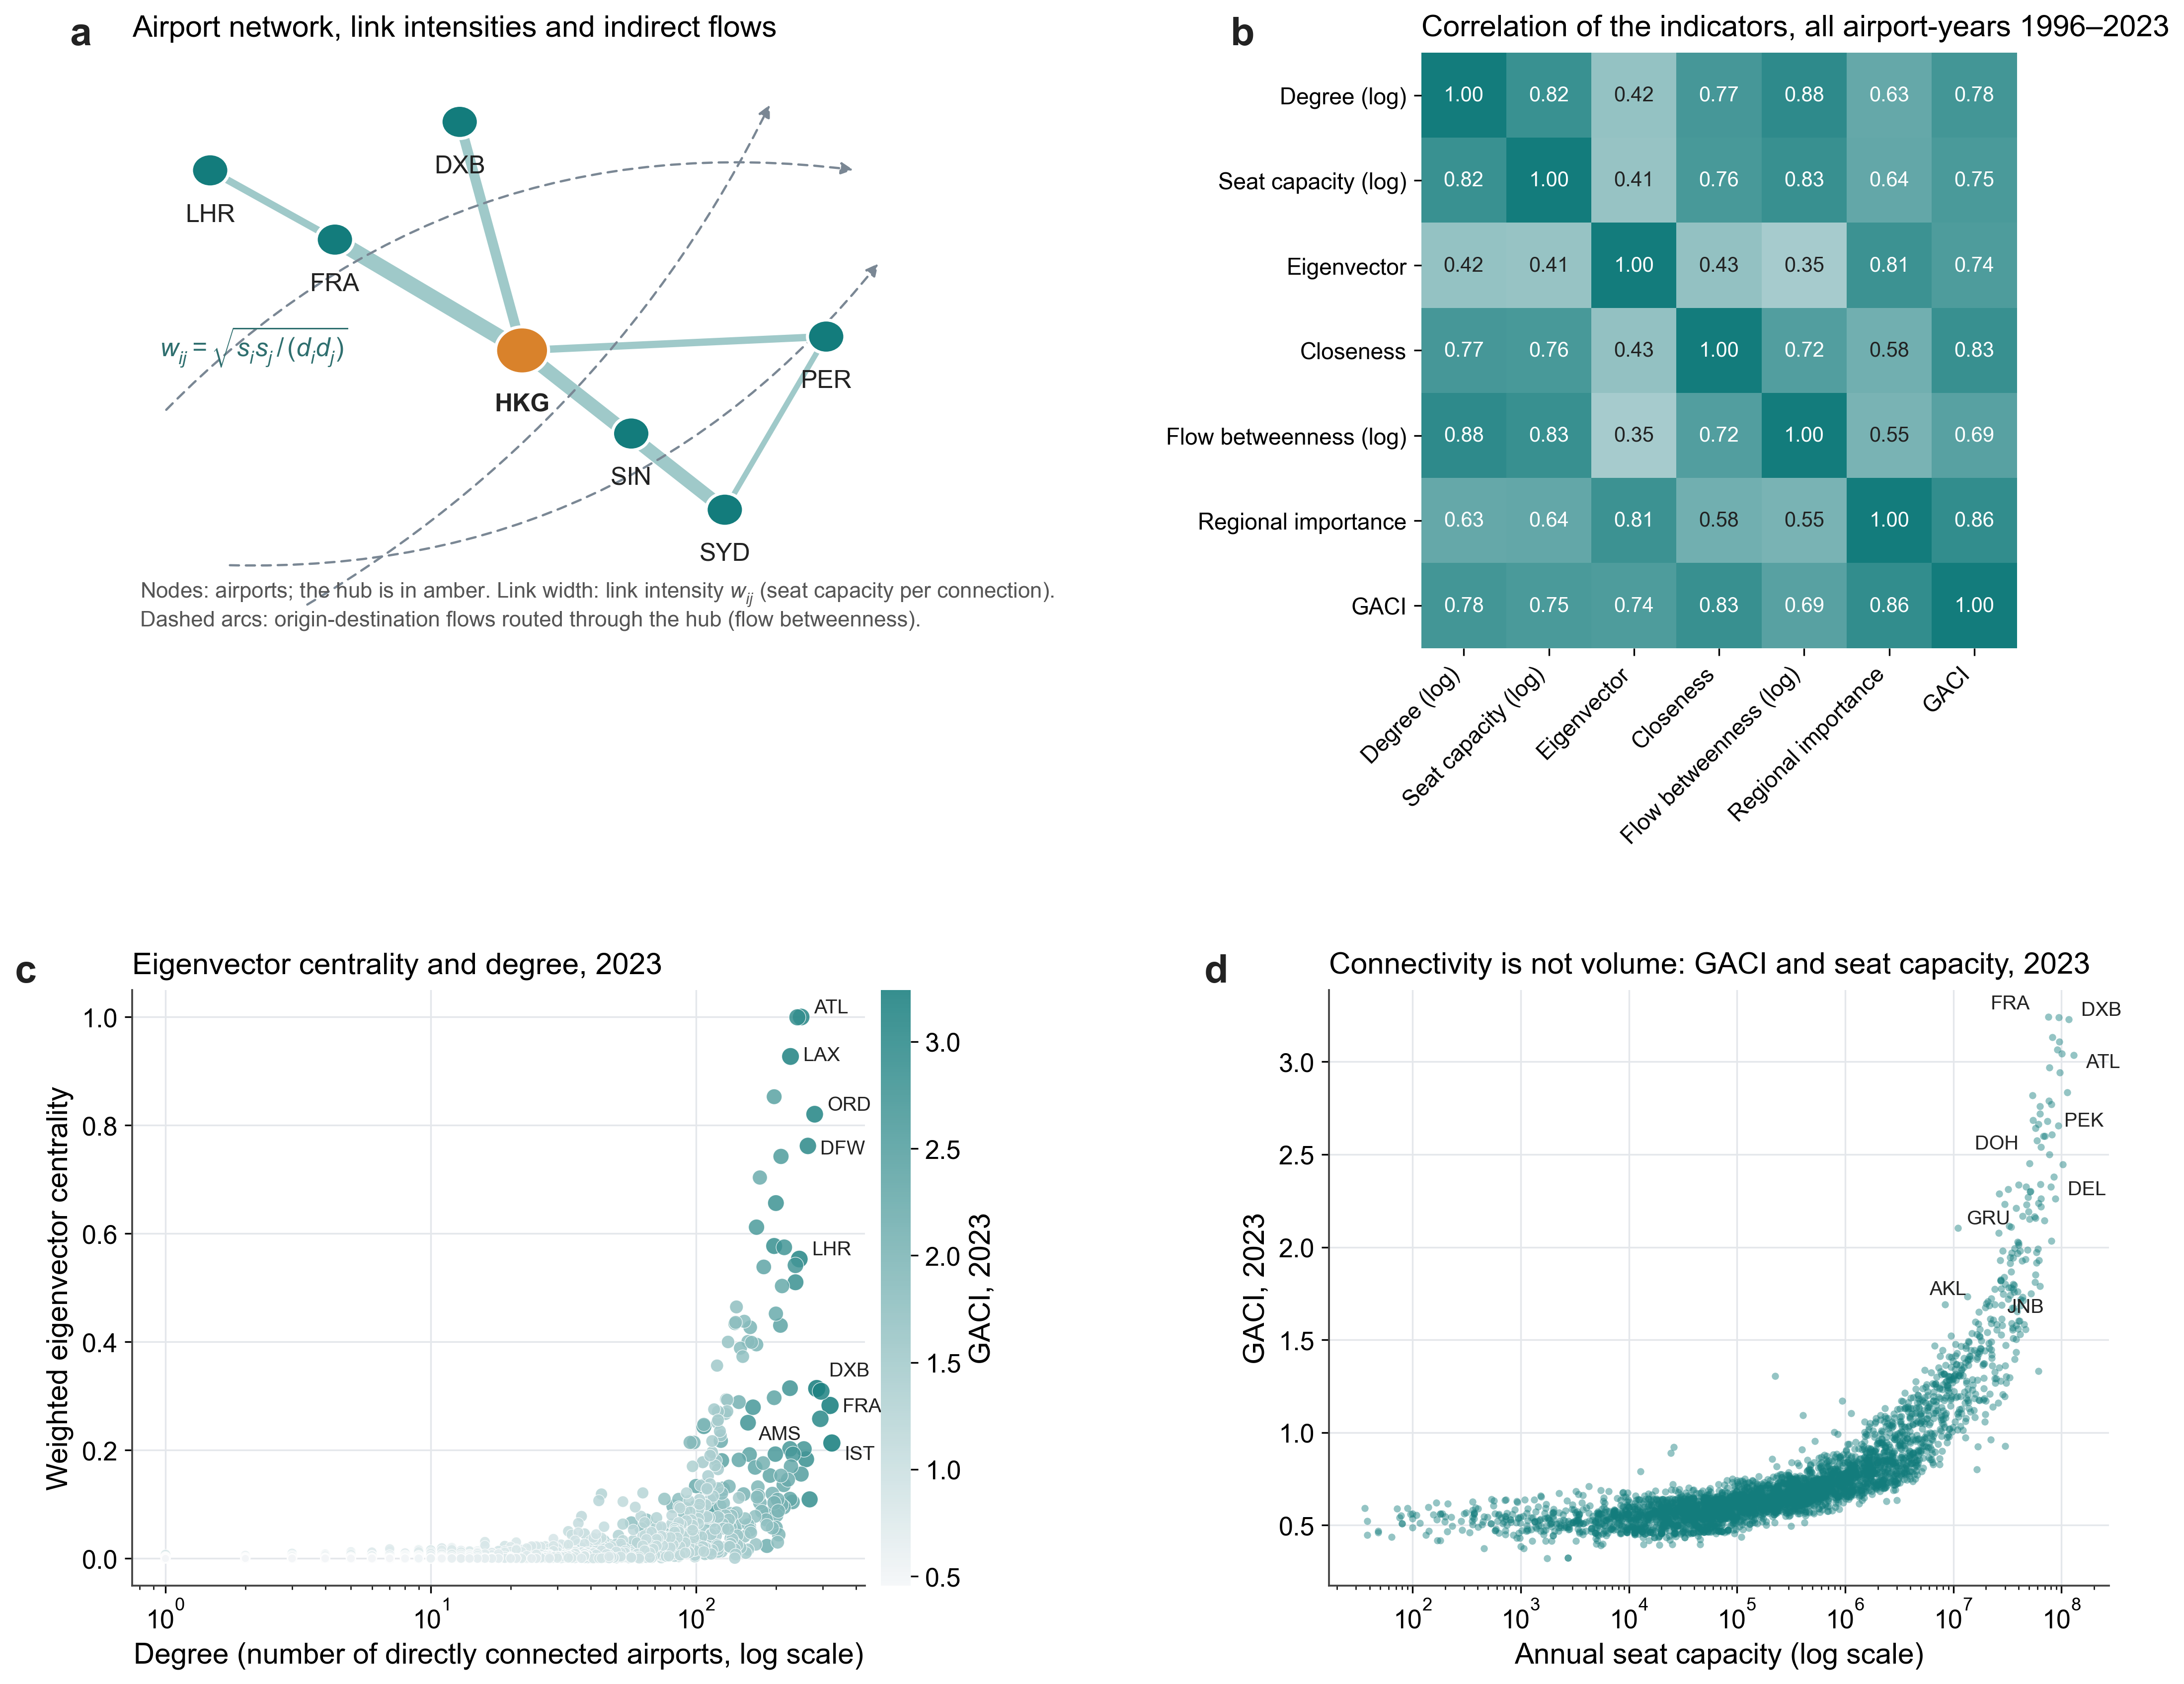
\includegraphics[width=\linewidth]{figures/FigB1_gaci_construction.png}
\caption{Construction of the connectivity index. (a) Schematic of the airport network: nodes are airports, the hub is in amber, link width is the link intensity $w_{ij}$, and dashed arcs are origin-destination flows routed through the hub. (b) Correlation matrix of the five indicators and the composite, all airport-years 1996--2023 (degree, seat capacity and flow betweenness in logs). (c) Weighted eigenvector centrality against degree, 2023, with colour and size proportional to GACI. (d) GACI against annual seat capacity, 2023. Source: authors' airport-year panel.}
\label{fig:construction}
\end{figure}

We aggregate the airport-level index to the country-year in three ways. Hub connectivity ($\mathrm{GACI}_{max}$) is the maximum across a country's airports, the connectivity of its primary gateway, and is the headline measure because the question of the paper concerns the hub. Hub quality ($\mathrm{GACI}_{cwm}$) is the seat-capacity-weighted mean, which uses the entire airport system while placing most weight on the dominant hubs. Total connectivity ($\mathrm{GACI}_{sum}$) is the sum across airports and blends hub connectivity with the size of the network. Two measures summarise the composition of the network: the share of the top airport in the national sum and the Herfindahl index of airport shares. The three aggregations are on different scales and their coefficients are not comparable one for one; what we use is the pattern of signs and significance across them, and the difference between the hub and the sum, which identifies the network net of the hub.

\paragraph{Inequality}
Inequality is measured from two sources. The Standardized World Income Inequality Database (SWIID, version 9) provides Gini coefficients of market income (before taxes and transfers) and of disposable income (after taxes and transfers), harmonised across countries and years to the Luxembourg Income Study standard \citep{Solt_2020}. Because the two are measured on the same footing, their difference, the redistribution wedge, measures the redistribution achieved by taxes and transfers. The World Inequality Database (WID) provides the distribution of pretax national income across equal-split adults, from which we take the average income and the income share of each decile, of the top percentile and top 0.1 percent, and of the bottom 50 percent and the middle 40 percent \citep{WID_2024}. The WID series are built on the distributional national accounts method of \citet{Piketty_2017}, which reconciles survey, tax and national-accounts data so that the group incomes sum to national income; this is what allows the incidence analysis of Section~\ref{sec:incidence}, in which the elasticity of mean income is exactly the income-share-weighted average of the group elasticities. From the same decile data we compute three further inequality measures used in robustness: the Palma ratio (the top-decile share over the bottom-40 share), the ratio of the top- to the bottom-decile mean income, and the absolute gap between the top-decile and bottom-half average incomes in constant local prices.

\paragraph{Instrument and other variables}
The instrument combines two components. The exposure is a country's air market access in the base year, $\mathrm{MA}^{air}_{c,1996}$, the population-weighted great-circle market access of its airports to the rest of the world, which depends on geography and on the 1996 distribution of world population. The shifter is a global aviation-intensity index $a_t$, normalised to $[0,1]$, that tracks the world expansion of scheduled air service over the sample period. Their interaction, $Z_{ct}=a_t\times\ln\mathrm{MA}^{air}_{c,1996}$, is the Feyrer instrument described in Section~\ref{sec:strategy}. Population and GDP per capita (constant 2015 US dollars) come from the World Development Indicators, as do the candidate mediators of Section~\ref{sec:mechanism}: sectoral employment shares, urbanisation, urban primacy, trade and FDI relative to GDP, tax revenue, unemployment, private credit, natural-resource rents and international tourist arrivals. The composition of trade (the share of differentiated goods under the Rauch classification, the value of high value-to-weight trade and the number of export partners) is computed from BACI, and the labour share from the Penn World Table. Neighbour definitions for the spillover analysis use contiguity, great-circle distance between country centroids and nearest-neighbour sets.

\paragraph{Sample and descriptive statistics}
The estimation sample is the intersection of the connectivity panel with the SWIID: 166 economies and 3{,}735 country-years over 1996--2023 for the Gini outcomes, and 3{,}714 country-years for the WID decile outcomes. Table~\ref{tab:sumstat} reports summary statistics. Two features of the data matter for what follows. First, inequality is slow moving: the within-country standard deviation of the market Gini is 1.7 points against a cross-sectional standard deviation of 6.4, so the identifying variation is a small fraction of the total. Second, hub connectivity also varies mainly across countries: its within standard deviation is 0.16 index units against 0.61 overall. Both features mean that the estimates rest on gradual within-country movements, and both explain why the inference reported below is clustered by country and, in robustness, allows for spatial correlation between countries.

\begin{table}[H]
\centering
\caption{Summary statistics, estimation sample (166 economies, 1996--2023).}
\label{tab:sumstat}
\begin{threeparttable}
\small
\begin{tabular}{lrrrrrr}
\toprule
Variable & N & Mean & SD & Within SD & Min & Max \\
\midrule
Market-income Gini (SWIID) & 3{,}737 & 45.594 & 6.413 & 1.672 & 31.200 & 72.400 \\
Disposable-income Gini (SWIID) & 3{,}737 & 38.363 & 8.193 & 1.678 & 22.100 & 65.800 \\
Top 10\% pretax income share (WID) & 3{,}716 & 0.453 & 0.093 & 0.025 & 0.255 & 0.687 \\
Bottom 50\% pretax income share (WID) & 3{,}716 & 0.150 & 0.047 & 0.012 & 0.051 & 0.279 \\
Hub connectivity, GACI max & 3{,}737 & 1.319 & 0.612 & 0.157 & 0.534 & 3.626 \\
Hub quality, GACI cwm & 3{,}737 & 1.124 & 0.416 & 0.115 & 0.534 & 3.014 \\
Total connectivity, GACI sum & 3{,}737 & 16.589 & 46.228 & 6.274 & 0.545 & 510.036 \\
Share of top airport in national GACI & 3{,}737 & 0.366 & 0.329 & 0.105 & 0.006 & 1.000 \\
Airports per country & 3{,}737 & 22.272 & 57.942 & 6.996 & 1.000 & 614.000 \\
Feyrer instrument & 3{,}737 & 4.606 & 4.227 & 4.104 & 0.000 & 14.667 \\
ln population & 3{,}737 & 16.095 & 1.805 & 0.125 & 9.778 & 21.078 \\
ln GDP per capita & 3{,}737 & 8.587 & 1.446 & 0.222 & 5.426 & 11.630 \\
\bottomrule
\end{tabular}
\begin{tablenotes}\small
\item Within SD is the standard deviation after removing country means. SWIID Gini coefficients in points (0--100); WID income shares as fractions of pretax national income (equal-split adults); GACI in index units; the Feyrer instrument is $a_t\times\ln\mathrm{MA}^{air}_{c,1996}$.
\end{tablenotes}
\end{threeparttable}
\end{table}


Figure~\ref{fig:maps} maps the geography of hub connectivity. Panel (a) plots every airport with scheduled service in 2023, with point size proportional to its index: the network is dense in North America, Europe and East Asia, and its largest nodes are the gateways of those regions together with Istanbul, Dubai, Jeddah and Singapore. Panel (b) aggregates to the country and shows the headline measure, $\ln\mathrm{GACI}_{max}$. The gateway economies of North America, Western Europe, the Gulf and East Asia occupy the top of the distribution and most of sub-Saharan Africa and Central Asia the bottom. Appendix Figure~\ref{fig:mapchange} maps the change in $\ln\mathrm{GACI}_{max}$ over the period, which is the variation the regressions use: hub connectivity rose most in Turkey, Korea, the Gulf, Ireland, Norway and much of South and East Asia, and fell in Russia, Venezuela and parts of Southern Africa.

\begin{figure}[H]
\centering
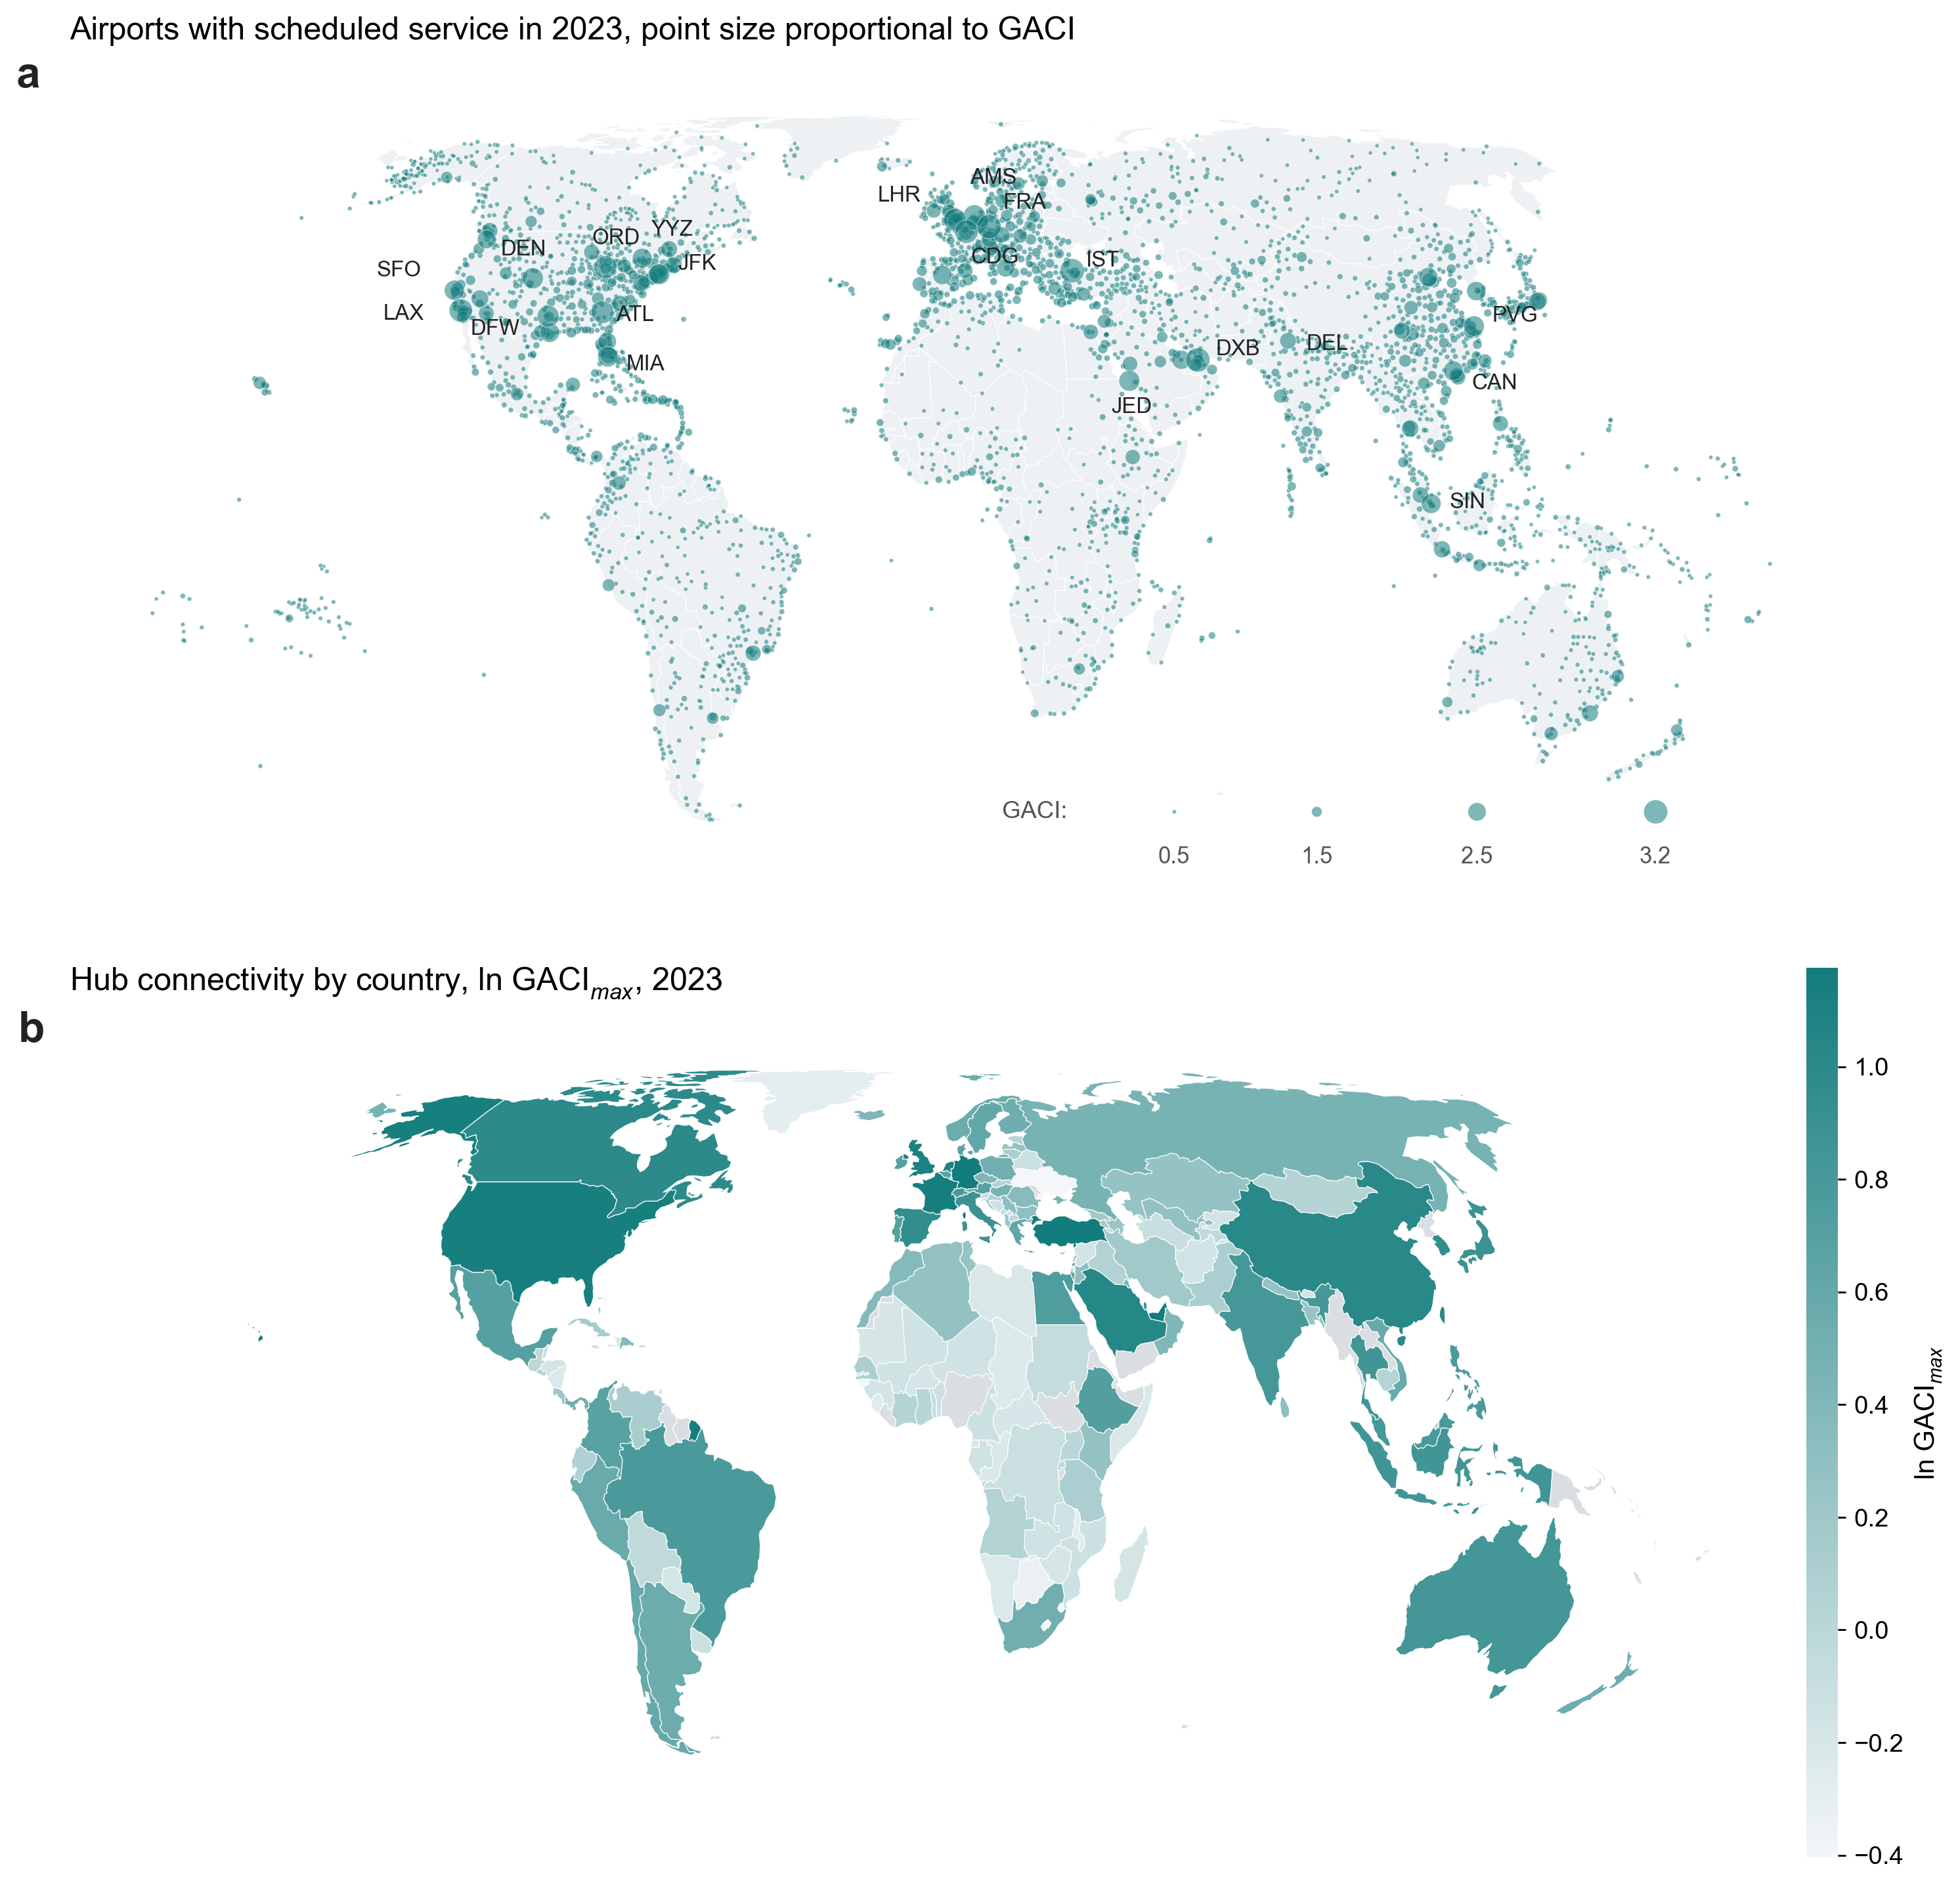
\includegraphics[width=0.92\linewidth]{figures/FigB3_maps_hubs.png}
\caption{The geography of hub connectivity, 2023. (a) Airports with scheduled service in 2023 (3{,}826 airports), point size proportional to GACI; the twenty most connected airports are labelled. (b) Hub connectivity by country, $\ln\mathrm{GACI}_{max}$, latest year; grey denotes economies outside the estimation sample. Equal Earth projection.}
\label{fig:maps}
\end{figure}

\paragraph{A first look at incidence}
Before turning to the estimates, Figure~\ref{fig:descriptive} shows the raw pattern that motivates the paper. For the 138 countries with at least fifteen years of decile data, we compute the annualised growth of the average pretax income of each decile and group countries into terciles of the annualised growth of hub connectivity over the same window. Panel (a) plots the mean growth rate of each group for the high, middle and low connectivity-growth terciles, in the manner of the growth incidence curves of \citet{Ravallion_2003} and \citet{Alvaredo_2018}. Countries whose hubs grew fastest grew faster at every point of the distribution, but the gap widens with rank: panel (b) shows that the high-minus-low difference is about 1.2 percentage points per year for the bottom decile, about 1.5 points across the middle of the distribution, 2.1 points for the top decile and 2.4 points for the top percentile. The raw curve is descriptive and confounded by everything that moves both connectivity and growth; the rest of the paper asks whether the tilt survives a design that isolates exogenous variation in connectivity.

\begin{figure}[H]
\centering
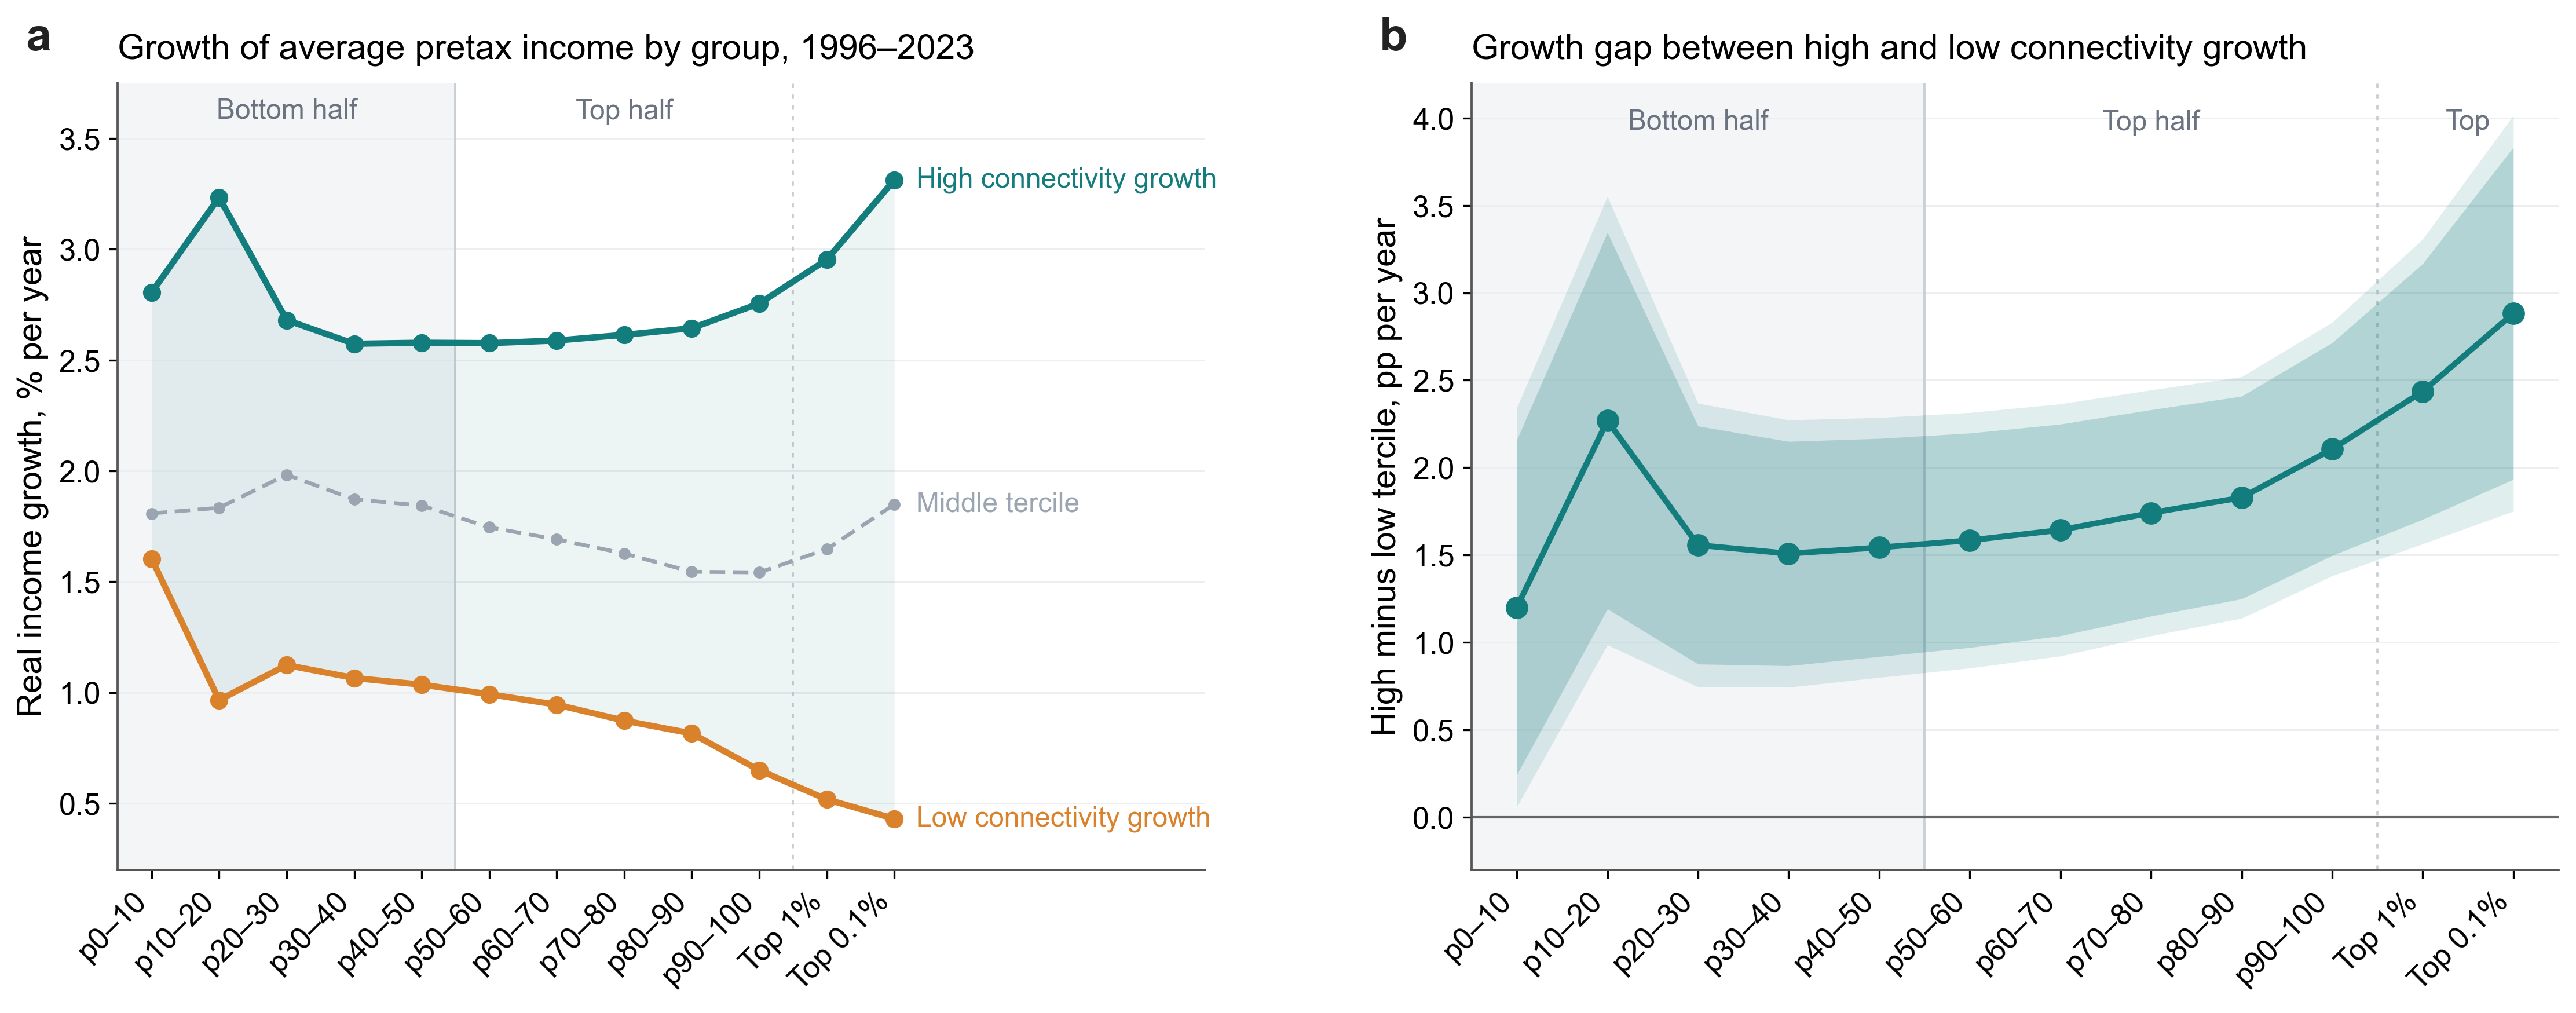
\includegraphics[width=\linewidth]{figures/Fig4_descriptive_v3.png}
\caption{Descriptive growth incidence by hub-connectivity growth, 1996--2023. (a) Mean annualised real growth of average pretax income by WID group for countries in the high, middle and low terciles of annualised growth in $\ln\mathrm{GACI}_{max}$ (46 countries per tercile; countries with at least fifteen years of decile data); the shaded area between the high and low terciles is the growth gap. (b) Difference between the high and low terciles; the dark and light bands are 90 and 95 percent confidence intervals. The grey panel marks the bottom half of the distribution. Source: WID and authors' connectivity panel.}
\label{fig:descriptive}
\end{figure}

%=======================================================================
\section{Empirical strategy}
\label{sec:strategy}
%=======================================================================
To estimate the impact of hub connectivity on within-country inequality, we estimate the following model:
\begin{equation}
y_{ct} = \beta\,\ln\mathrm{GACI}_{ct} + \gamma\,\ln\text{pop}_{ct} + \alpha_c + \delta_t + \varepsilon_{ct},
\label{eq:main}
\end{equation}
where $y_{ct}$ is the natural logarithm of an inequality outcome of country $c$ in year $t$: the market-income Gini ($\ln G^{mkt}$), the disposable-income Gini ($\ln G^{disp}$), or, in the incidence analysis, the average pretax income or the income share of a group of the distribution. $\ln\mathrm{GACI}_{ct}$ is the natural logarithm of hub connectivity ($\mathrm{GACI}_{max}$) in the headline specification, and of hub quality ($\mathrm{GACI}_{cwm}$) or total connectivity ($\mathrm{GACI}_{sum}$) in the alternatives. The model includes country fixed effects ($\alpha_c$) and year fixed effects ($\delta_t$). Population is the only time-varying control, for the same reason as in the companion papers: the country fixed effects absorb all time-invariant determinants of inequality, and the natural time-varying candidates, GDP per capita, urbanisation, the sectoral structure and trade, are themselves outcomes of connectivity (Section~\ref{sec:mechanism}), so conditioning on them would control away part of the effect of interest. They enter instead as candidate mechanisms. Because $\beta$ is an elasticity, a coefficient of $0.5$ on the market Gini means that a 10 percent increase in hub connectivity raises the Gini by 5 percent, or about 2.3 points at the sample mean of 45.6.

Identifying the causal effect of connectivity on inequality is difficult for two reasons. First, connectivity is poorly represented by a binary treatment. A country's hub gains connectivity continuously, through frequencies, partner growth and the growth of the partners' own networks, rather than through discrete, datable events; a continuous, network-based index that embeds partner-of-partner connections is the appropriate measurement. Second, the variation that does exist is endogenous: airlines add capacity where income is growing, and the reforms that attract them may also change the distribution of income directly. We therefore instrument connectivity with the Feyrer interaction
\begin{equation}
Z_{ct} = a_t \times \ln\mathrm{MA}^{air}_{c,1996},
\label{eq:iv}
\end{equation}
where $a_t$ is the global aviation-intensity index and $\mathrm{MA}^{air}_{c,1996}$ is the country's air market access in the base year \citep{Feyrer_2019}. The logic is that of \citet{Feyrer_2019}: as aviation expanded worldwide, countries whose geography placed them nearer, by air, to the rest of the world's population gained connectivity by more, for reasons that have nothing to do with their own income distribution. The instrument has the shift-share structure of \citet{GoldsmithPinkham_2020}, \citet{Adao_2019} and \citet{Borusyak_2022} with a single global shifter and a predetermined exposure. Country fixed effects absorb the exposure, year fixed effects absorb the shifter, and identification rests on their interaction alone. The identifying assumption is that, conditional on the fixed effects, countries with higher baseline air market access did not experience differential inequality trends for reasons other than connectivity. Section~\ref{sec:robust} examines this assumption by allowing other baseline characteristics (income, inequality, land area, latitude and sea market access) to have their own trends in the aviation index.

The first-stage regression is
\begin{equation}
\ln\mathrm{GACI}_{ct} = \pi_1 Z_{ct} + \pi_2 \ln\text{pop}_{ct} + \mu_c + \lambda_t + \nu_{ct},
\label{eq:first}
\end{equation}
and the second stage replaces $\ln\mathrm{GACI}_{ct}$ in Equation~\eqref{eq:main} with its fitted value. We report the Kleibergen--Paap $rk$ Wald statistic (KP $F$) for every 2SLS estimate. Because inequality and connectivity are both persistent and move slowly, the errors of Equation~\eqref{eq:main} are serially correlated within countries, and we cluster standard errors by country throughout. Countries are also spatially dependent, so in robustness we report Conley standard errors \citep{Conley_1999} with a Bartlett kernel in great-circle distance between country centroids at cutoffs of 1{,}000 and 2{,}000 km, allowing arbitrary within-country serial correlation, and two-way clustering by country and year.

For additional analyses, we examine (1) the incidence of connectivity across the income distribution, (2) growth and inequality by baseline hub size, (3) the mechanisms through which hub connectivity acts on inequality, and (4) the aggregate contribution of connectivity growth to within-country inequality over 1996--2023.

For (1), we estimate Equation~\eqref{eq:main} separately for the log average pretax income of each WID group $g$ (ten deciles, the top 1 and top 0.1 percent, the bottom 50 and the middle 40 percent) and for its log income share. Because the WID groups exhaust national income, the log income share is the log group income minus the log mean income of all adults, so the share elasticity is the group elasticity minus the mean-income elasticity, and all groups are estimated on the same sample. The set of group elasticities plotted against rank is the instrumented counterpart of the growth incidence curve \citep{Ravallion_2003}. To test differences between groups exactly, we regress the difference of two group outcomes (for example, the log income of the top decile minus the log income of the bottom half) on instrumented connectivity, which gives the difference of the two elasticities with its standard error; and we stack all groups in one system with group-specific connectivity coefficients, group-specific instruments and country-by-group and year-by-group fixed effects, which allows a joint test of equal elasticities and a test of a linear trend in the elasticity across deciles.

For (2), we ask whether connectivity raises income and inequality together, and where. We split countries on their baseline hub connectivity ($\mathrm{GACI}_{max}$ in 1996 or the earliest observed year) at the median and into terciles (and, in the appendix, into quartiles and under alternative base years and measures), and estimate Equation~\eqref{eq:main} by 2SLS within each group for GDP per capita, WID mean income and the two Gini coefficients. We use split samples rather than an interaction model because the instrument's power differs sharply across groups: the Feyrer interaction moves the connectivity of hubs that are integrating into the network and has little purchase on hubs that were already among the world's largest in 1996. Reporting the first-stage statistic for each group makes this visible, and we interpret only groups in which the instrument has power. The same logic governs the heterogeneity splits by urbanisation, tourism dependence and trade openness, each at the median of the earliest observed value.

For (3), we ask five questions, each with a regression. First, which connectivity carries the effect: we enter hub connectivity together with total connectivity or with the connectivity of the country's secondary airports as a control, and we instrument individual components of hub connectivity (eigenvector centrality, seat capacity, degree, closeness, flow betweenness, regional importance) one at a time and in pairwise horse races. Second, who gains: the incidence regressions of (1), summarised by the mean income, the income of the bottom half and the top decile, the bottom-half share and two ratios of decile mean incomes, the median to the bottom decile (p50/p10) and the top decile to the median (p90/p50). Third, whether the effect is a growth effect: for a candidate mediator $\mathrm{M}_{ct}$ we estimate
\begin{equation}
\mathrm{M}_{ct} = a\,\ln\mathrm{GACI}_{ct} + \kappa\,\ln\text{pop}_{ct} + \xi_c + \zeta_t + \phi_{ct},
\label{eq:mec1}
\end{equation}
\begin{equation}
y_{ct} = c'\,\ln\mathrm{GACI}_{ct} + b\,\mathrm{M}_{ct} + \gamma\,\ln\text{pop}_{ct} + \alpha_c + \delta_t + \varepsilon_{ct},
\label{eq:mec2}
\end{equation}
with connectivity instrumented in both. If the effect on inequality ran through the mediator, $a$ and $b$ would carry the same sign and $c'$ would fall short of the total effect $\beta$. As in the companion paper, this is a descriptive decomposition rather than a formal causal mediation: the mediator is itself an outcome of connectivity and is then entered as a regressor, so $c'$ is the connectivity coefficient conditional on the mediator and $b$ an association, not a structural effect. We apply the decomposition to GDP per capita in the main text and to eighteen candidate mediators in the appendix. Fourth, where the effect is found: split samples by urbanisation, tourism dependence, trade openness and baseline hub size, and a spillover regression in which own connectivity and the leave-out mean of contiguous (or nearby) neighbours' connectivity enter jointly, each instrumented by its own shifter. Fifth, whether redistribution offsets the effect: the disposable Gini, the redistribution wedge (market minus disposable Gini, in points), its log ratio, and tax revenue relative to GDP.

For (4), we quantify the aggregate contribution of connectivity growth by multiplying each country's observed change in $\ln\mathrm{GACI}_{max}$ between its first and last year with complete data by the 2SLS elasticities, for the Gini and for the income and share of each group, and aggregating across countries with and without population weights (Section~\ref{sec:aggregate}).

%=======================================================================
\section{Main results}
\label{sec:results}
%=======================================================================
\subsection{Hub connectivity and inequality}
\label{sec:headline}
We first ask whether hub connectivity raised within-country inequality. Table~\ref{tab:main} reports, for each of our three measures of connectivity, three lines side by side: the first-stage relevance of the instrument, the OLS association, and the instrumented (2SLS) estimate, for the market-income and the disposable-income Gini. Reading down each panel shows how isolating exogenous variation changes the picture. The three measures agree in sign and significance, and we adopt hub connectivity ($\ln\mathrm{GACI}_{max}$) as the headline because the hypotheses concern the hub; hub quality and total connectivity serve as robustness measures and, in Section~\ref{sec:mechanism}, to separate the hub from the network.

\begin{table}[H]
\centering
\caption{Main results: OLS, first stage, and 2SLS, by connectivity measure.}
\label{tab:main}
\begin{threeparttable}
\small
\begin{tabular}{lcc}
\toprule
 & Market-income Gini & Disposable-income Gini \\
 & $\ln G^{mkt}$ & $\ln G^{disp}$ \\
\midrule
\multicolumn{3}{l}{\emph{Panel A. Hub connectivity, $\ln\mathrm{GACI}_{max}$ (headline)}}\\
First stage: instrument coef. & \multicolumn{2}{l}{0.146\sym{***}\ \ (0.045),\ \ KP $F=10.6$} \\
OLS & 0.061\sym{***} & 0.050\sym{*} \\
 & (0.023) & (0.026) \\
2SLS & 0.495\sym{**} & 0.651\sym{***} \\
 & (0.194) & (0.241) \\
\addlinespace
\multicolumn{3}{l}{\emph{Panel B. Hub quality, $\ln\mathrm{GACI}_{cwm}$}}\\
First stage: instrument coef. & \multicolumn{2}{l}{0.122\sym{***}\ \ (0.041),\ \ KP $F=8.8$} \\
OLS & 0.079\sym{***} & 0.060\sym{**} \\
 & (0.026) & (0.030) \\
2SLS & 0.595\sym{**} & 0.783\sym{***} \\
 & (0.240) & (0.302) \\
\addlinespace
\multicolumn{3}{l}{\emph{Panel C. Total connectivity, $\ln\mathrm{GACI}_{sum}$}}\\
First stage: instrument coef. & \multicolumn{2}{l}{0.364\sym{***}\ \ (0.086),\ \ KP $F=18.0$} \\
OLS & 0.008 & 0.009 \\
 & (0.007) & (0.009) \\
2SLS & 0.199\sym{***} & 0.262\sym{***} \\
 & (0.077) & (0.090) \\
\addlinespace
\midrule
Country, Year FE & Yes & Yes \\
Observations & 3{,}735 & 3{,}735 \\
\bottomrule
\end{tabular}
\begin{tablenotes}\small
\item Each panel instruments its connectivity measure with the Feyrer interaction. The first-stage row regresses the connectivity measure on the instrument with log population and two-way fixed effects; KP $F$ is the Kleibergen--Paap $rk$ Wald statistic with country-clustered errors. Country-year panel, 1996--2023. All regressions include country and year fixed effects and log population. 2SLS instruments ln GACI with the Feyrer interaction $Z_{ct}=a_t\times\ln \mathrm{MA}^{air}_{c,1996}$. Standard errors clustered by country in parentheses. \sym{*}~$p<0.10$, \sym{**}~$p<0.05$, \sym{***}~$p<0.01$.
\end{tablenotes}
\end{threeparttable}
\end{table}


Panel A uses hub connectivity. The instrument is a strong predictor of connectivity: it enters the first stage with the expected positive sign ($0.146$, $p<0.01$) and a Kleibergen--Paap statistic of $10.6$, at the conventional threshold. In OLS, a one percent increase in hub connectivity is associated with a $0.061$ percent increase in the market Gini ($p<0.01$) and a $0.050$ percent increase in the disposable Gini ($p<0.10$). The 2SLS estimates are an order of magnitude larger: $0.495$ for the market Gini ($p<0.05$) and $0.651$ for the disposable Gini ($p<0.01$). A coefficient of $0.495$ means that a 10 percent increase in hub connectivity raises the market Gini by about 5 percent, or 2.3 points at the sample mean of 45.6; one within-country standard deviation of hub connectivity, about 12 percent of the mean, raises it by 2.7 points, which is more than one and a half times the within-country standard deviation of the Gini itself. That the 2SLS estimate exceeds the OLS estimate is what the mechanism of Section~\ref{sec:mechanism} implies: the growth that connectivity generates is itself associated with lower inequality, so the OLS coefficient nets a disequalising direct effect against an equalising growth effect, whereas the instrument isolates the variation in connectivity that arrives through the global network rather than through domestic growth. These estimates bear directly on \textbf{Hypothesis~1}, which predicts that hub connectivity increases within-country inequality. \textbf{Hypothesis~1} is supported for both the market and the disposable Gini.

Panel B uses hub quality ($\ln\mathrm{GACI}_{cwm}$), the capacity-weighted mean across the airport system, and Panel C total connectivity ($\ln\mathrm{GACI}_{sum}$). The signs and significance carry over: 2SLS elasticities of $0.595$ and $0.783$ for hub quality ($p<0.05$ and $p<0.01$) and $0.199$ and $0.262$ for total connectivity (both $p<0.01$). The first stage is strongest for the sum ($F=18.0$), since the global aviation cycle moves every airport in the country, and the coefficient on the sum is correspondingly smaller because the sum blends the hub with the rest of the network. The three measures are on different scales and cannot be compared coefficient for coefficient; what carries over is the common pattern of signs and significance, so that the support for \textbf{Hypothesis~1} is not an artefact of any one aggregation of connectivity. The difference between the hub and the sum is the subject of Section~\ref{sec:mechanism}.

%=======================================================================
\subsection{Incidence across the income distribution}
\label{sec:incidence}
The Gini is a summary statistic, so we next ask which part of the distribution moves. Table~\ref{tab:incidence} and Figure~\ref{fig:incidence} report the 2SLS elasticity of the average pretax income of each WID group (left columns) and of its income share (right columns) to hub connectivity; each cell is a separate regression on the same 3{,}714 country-years, so the coefficients are directly comparable across rows.

\begin{table}[H]
\centering
\caption{Incidence of hub connectivity across the income distribution (2SLS, Feyrer instrument).}
\label{tab:incidence}
\begin{threeparttable}
\small
\begin{tabular}{lcccc}
\toprule
 & \multicolumn{2}{c}{Average income of the group} & \multicolumn{2}{c}{Income share of the group} \\
\cmidrule(lr){2-3}\cmidrule(lr){4-5}
WID group & Coef. & (s.e.) & Coef. & (s.e.) \\
\midrule
\multicolumn{5}{l}{\emph{Panel A. Elasticity to $\ln\mathrm{GACI}_{max}$, 2SLS}}\\
p0--10 & 0.155 & (1.695) & -1.061 & (1.545) \\
p10--20 & -1.931 & (2.204) & -3.146 & (2.239) \\
p20--30 & -0.021 & (0.698) & -1.240\sym{**} & (0.619) \\
p30--40 & 0.537 & (0.578) & -0.681\sym{*} & (0.376) \\
p40--50 & 0.693 & (0.549) & -0.526\sym{*} & (0.307) \\
p50--60 & 0.887 & (0.548) & -0.331 & (0.241) \\
p60--70 & 1.052\sym{*} & (0.546) & -0.167 & (0.184) \\
p70--80 & 1.194\sym{**} & (0.537) & -0.024 & (0.141) \\
p80--90 & 1.335\sym{**} & (0.537) & 0.116 & (0.128) \\
p90--100 & 1.443\sym{***} & (0.513) & 0.224 & (0.192) \\
Top 1\% & 1.285\sym{**} & (0.541) & 0.067 & (0.384) \\
Top 0.1\% & 0.578 & (0.695) & -0.640 & (0.676) \\
Bottom 50\% & 0.445 & (0.593) & -0.774\sym{*} & (0.417) \\
Middle 40\% & 1.179\sym{**} & (0.534) & -0.039 & (0.136) \\
All adults (mean income) & 1.219\sym{**} & (0.491) & -- &  \\
\addlinespace
\multicolumn{5}{l}{\emph{Panel B. Differences between groups (difference outcomes)}}\\
p90--100 minus bottom 50\% & 0.998\sym{*} & (0.588) & & \\
Top half (p50--100) minus bottom half (p0--50) & 1.259\sym{*} & (0.755) & & \\
p90--100 minus p0--10 & 1.281 & (1.615) & & \\
Top 1\% minus p90--100 & -0.157 & (0.274) & & \\
\midrule
First-stage KP $F$ & \multicolumn{2}{c}{10.5} & \multicolumn{2}{c}{10.5} \\
Observations & \multicolumn{2}{c}{3{,}714} & \multicolumn{2}{c}{3{,}714} \\
\bottomrule
\end{tabular}
\begin{tablenotes}\small
\item Each cell is a separate regression. Income is the log average pretax national income of the group (WID, equal-split adults); the share is the log income share, computed as log group income minus log mean income so that all groups use the same sample. Panel B regresses the difference of two group outcomes, which gives the exact difference of the two elasticities with its standard error. Country-year panel, 1996--2023. All regressions include country and year fixed effects and log population. 2SLS instruments ln GACI with the Feyrer interaction $Z_{ct}=a_t\times\ln \mathrm{MA}^{air}_{c,1996}$. Standard errors clustered by country in parentheses. \sym{*}~$p<0.10$, \sym{**}~$p<0.05$, \sym{***}~$p<0.01$.
\end{tablenotes}
\end{threeparttable}
\end{table}


\begin{figure}[H]
\centering
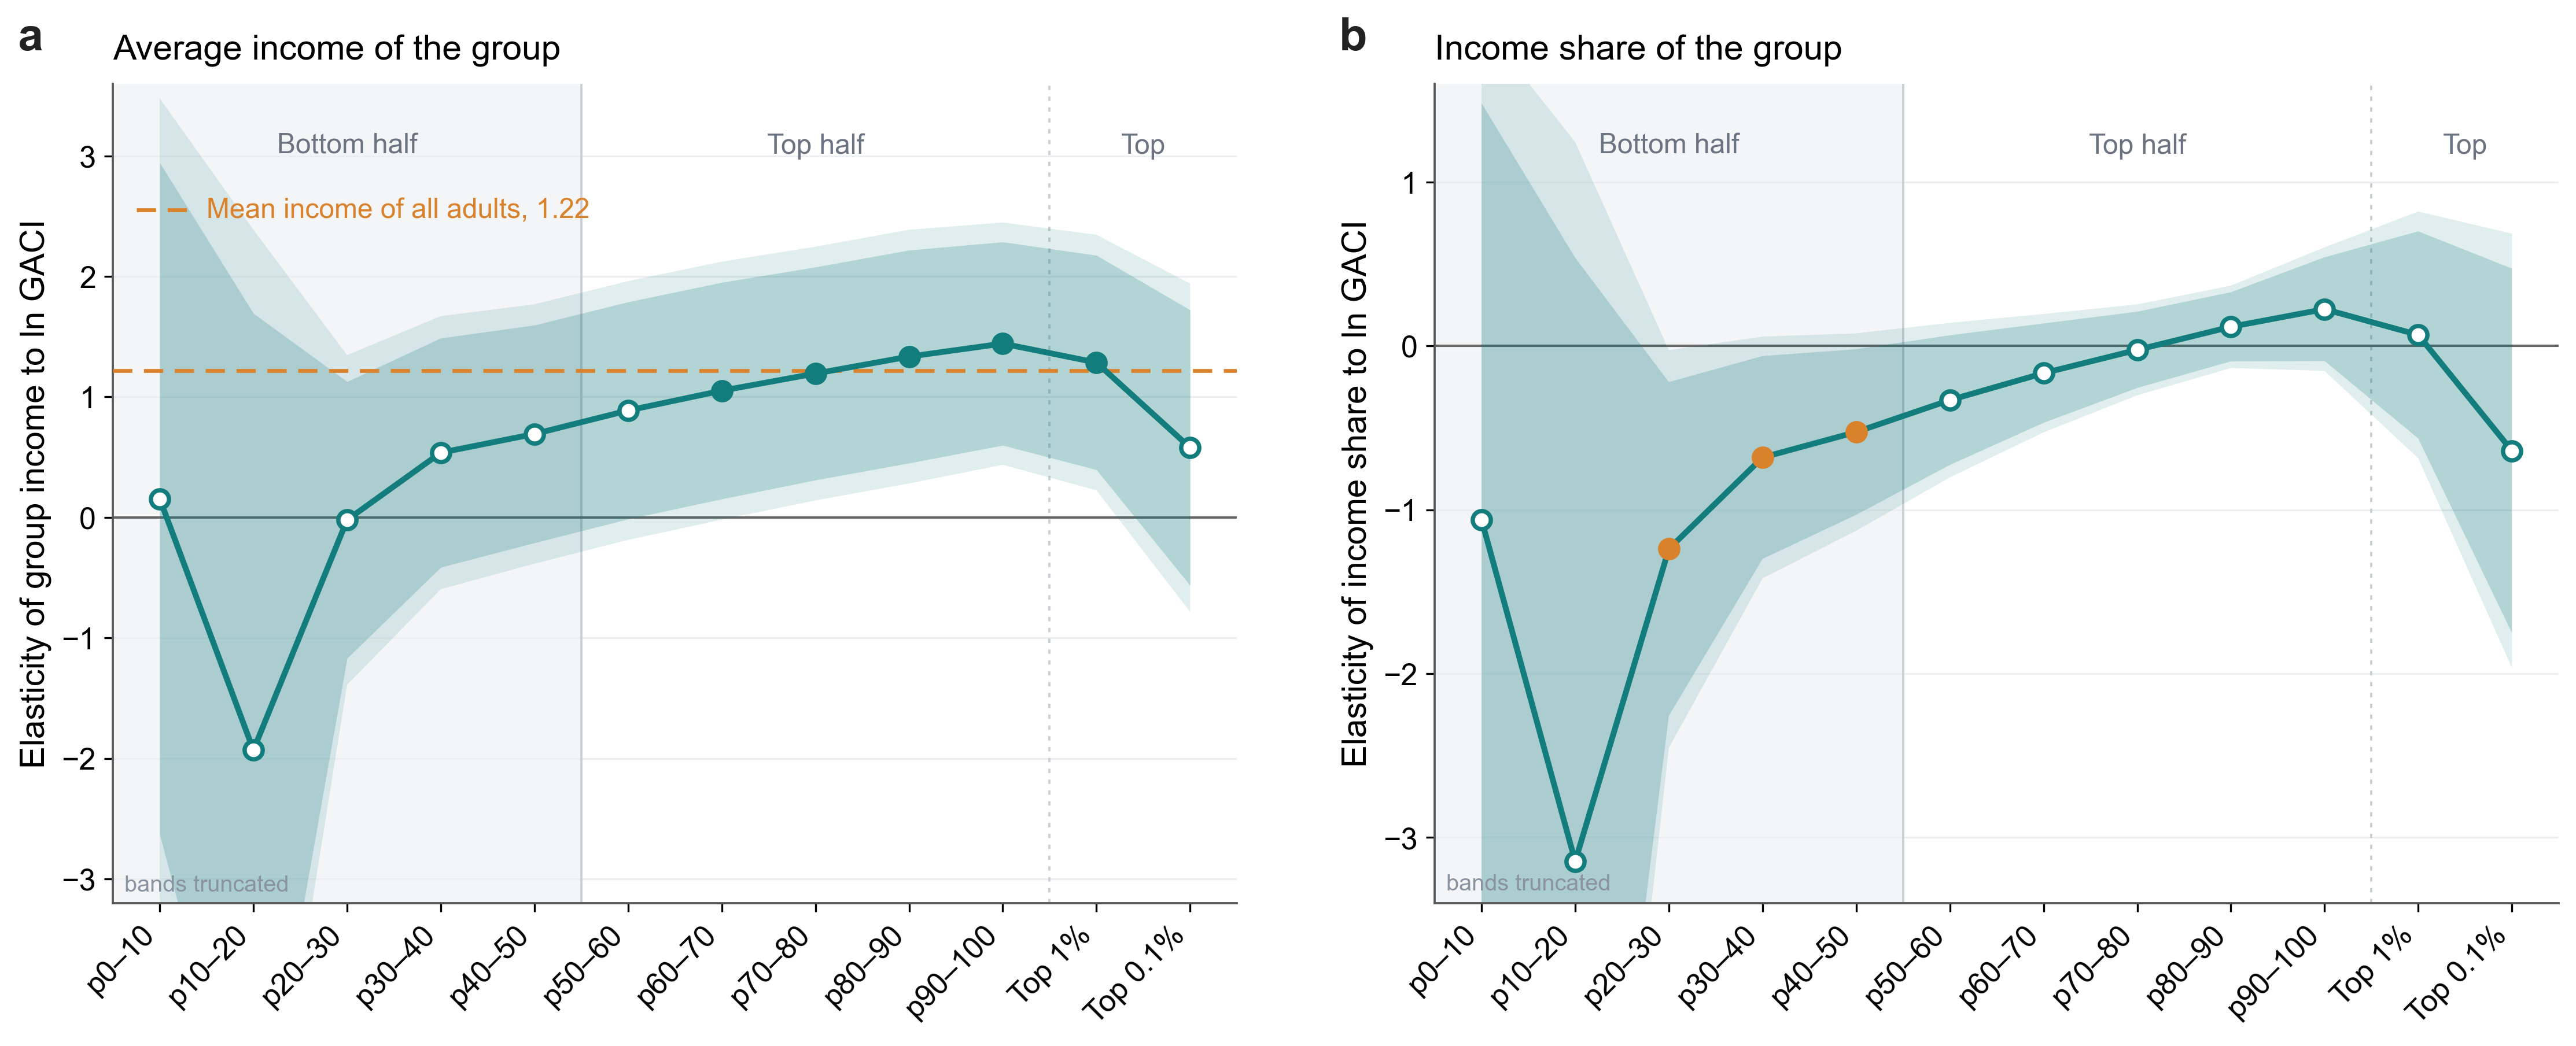
\includegraphics[width=\linewidth]{figures/Fig1_incidence_v3.png}
\caption{Incidence of hub connectivity across the income distribution (2SLS, Feyrer instrument). (a) Elasticity of the average pretax income of each WID group to $\ln\mathrm{GACI}_{max}$; the dashed line is the elasticity of mean income of all adults. (b) Elasticity of the group's income share. The line connects the point estimates of Table~\ref{tab:incidence}; the dark and light bands are 90 and 95 percent confidence intervals clustered by country, truncated at the axis limits for the two lowest deciles. Filled markers denote $p<0.10$; amber markers denote significant negative estimates. The grey panel marks the bottom half of the distribution.}
\label{fig:incidence}
\end{figure}

The pattern is a staircase. Mean income of all adults rises with an elasticity of $1.219$ ($p<0.05$), consistent with the GDP effect of the companion paper. From the seventh decile upward, group incomes rise with the mean: $1.052$ for p60--70 ($p<0.10$), $1.194$ for p70--80 and $1.335$ for p80--90 (both $p<0.05$) and $1.443$ for the top decile ($p<0.01$). Below the median none of the elasticities is distinguishable from zero, and the bottom half as a whole has an elasticity of $0.445$ with a standard error of $0.593$. The share columns show the same movement from the other side: the shares of the third, fourth and fifth deciles fall (elasticities of $-1.240$, $-0.681$ and $-0.526$, $p<0.05$, $p<0.10$ and $p<0.10$), the bottom-half share falls with an elasticity of $-0.774$ ($p<0.10$), and the top-decile share rises but not significantly ($0.224$). Panel B reports the differences exactly: the top-decile income rises by $0.998$ more than the bottom-half income ($p<0.10$), and the upper half by $1.259$ more than the lower half ($p<0.10$). The stacked system of Appendix Table~\ref{tab:a_stacked} confirms the halves contrast ($1.296$, $p<0.10$); the joint test of equal elasticities across all ten deciles does not reject, which reflects the imprecision of the bottom two deciles rather than a flat curve, since the significant contrasts are those between the halves.

Two features of the staircase identify the mechanism. First, the growth that connectivity generates is not ordinary growth in the sense of \citet{Dollar_2016}: under their benchmark the bottom half would rise one-for-one with the mean, whereas here it does not rise at all. Second, the top does not pull away from the upper-middle. The top percentile's elasticity ($1.285$) is below that of the top decile, the top 0.1 percent's is smaller still and insignificant, and the difference between the top percentile and the top decile is $-0.157$ with a standard error of $0.274$. The response is broad across the upper half and absent in the lower half, the shape that sorting into the hub economy predicts, and not the concentration at the very top that skill-biased demand for the highest earners or innovation rents would produce \citep{Aghion_2018}. Table~\ref{tab:mech_B} below reports the corresponding ratios of decile means: the median-to-bottom-decile ratio (p50/p10) rises with an elasticity of $2.260$ ($p<0.05$) while the top-to-median ratio (p90/p50) does not move ($0.747$, standard error $0.485$). These results bear directly on \textbf{Hypothesis~2}, which predicts that the response is located in the lower half of the distribution and that the top percentile does not gain relative to the top decile. \textbf{Hypothesis~2} is supported on both counts.

%=======================================================================
\subsection{Growth and inequality by baseline hub size}
\label{sec:growthineq}
The companion paper finds the largest income gains from connectivity in the least developed economies. We ask whether the inequality response is located in the same economies, and whether growth and inequality respond together. Table~\ref{tab:growth_ineq} splits countries on the connectivity of their hub in 1996, at the median and into terciles, and reports, within each group, the 2SLS and OLS elasticities of GDP per capita, WID mean income, and the two Gini coefficients, together with the first-stage statistic; Appendix Table~\ref{tab:a_stagedefs} adds quartiles and alternative base years. Figure~\ref{fig:heterogeneity} plots the market-Gini elasticities by baseline connectivity tercile, baseline GDP tercile, region and era.

\begin{table}[p]
\centering
\caption{Growth and inequality by baseline hub size (countries grouped on $\mathrm{GACI}_{max}$ in 1996).}
\label{tab:growth_ineq}
\begin{threeparttable}
\footnotesize
\begin{tabular}{lcccccc}
\toprule
 & ln GDP p.c. & ln mean income & ln market Gini & ln disp. Gini & KP $F$ / N \\
\midrule
\multicolumn{6}{l}{\emph{Panel A. Median split}}\\
Below median (smaller hubs): 2SLS & 1.221\sym{***} & 1.318\sym{***} & 0.356\sym{***} & 0.399\sym{***} & 22.2 \\
 & (0.311) & (0.333) & (0.122) & (0.138) & N = 1{,}706 \\
\quad OLS & 0.570\sym{***} & 0.657\sym{***} & 0.082\sym{***} & 0.077 & \\
 & (0.169) & (0.195) & (0.030) & (0.048) & \\
Above median (larger hubs): 2SLS & 2.154 & 1.818 & 1.585 & 2.358 & 0.5 \\
 & (2.493) & (2.666) & (2.277) & (3.355) & N = 2{,}029 \\
\quad OLS & 0.857\sym{***} & 0.692\sym{***} & 0.062\sym{*} & 0.042 & \\
 & (0.164) & (0.175) & (0.035) & (0.034) & \\
\addlinespace
\multicolumn{6}{l}{\emph{Panel B. Terciles}}\\
Low: 2SLS & 1.719\sym{***} & 1.520\sym{***} & 0.122 & 0.152 & 19.7 \\
 & (0.384) & (0.307) & (0.096) & (0.116) & N = 1{,}048 \\
\quad OLS & 0.963\sym{***} & 1.034\sym{***} & 0.017 & 0.021 & \\
 & (0.124) & (0.118) & (0.042) & (0.070) & \\
Middle: 2SLS & 0.891\sym{*} & 0.739 & 0.554\sym{**} & 0.641\sym{**} & 8.1 \\
 & (0.476) & (0.580) & (0.219) & (0.257) & N = 1{,}310 \\
\quad OLS & 0.573\sym{**} & 0.470\sym{**} & 0.114\sym{***} & 0.095\sym{**} & \\
 & (0.225) & (0.218) & (0.031) & (0.039) & \\
High: 2SLS & 0.871 & 1.356 & 1.410 & 2.138 & 0.4 \\
 & (1.519) & (1.813) & (2.308) & (3.389) & N = 1{,}377 \\
\quad OLS & 0.847\sym{***} & 0.738\sym{***} & 0.035 & 0.021 & \\
 & (0.199) & (0.196) & (0.049) & (0.046) & \\
\addlinespace
\multicolumn{6}{l}{\emph{Reference}}\\
Full sample: 2SLS & 1.294\sym{***} & 1.219\sym{**} & 0.495\sym{**} & 0.651\sym{***} & 10.6 \\
 & (0.428) & (0.491) & (0.194) & (0.241) & N = 3{,}735 \\
\quad OLS & 0.747\sym{***} & 0.668\sym{***} & 0.061\sym{***} & 0.050\sym{*} & \\
 & (0.121) & (0.124) & (0.023) & (0.026) & \\
\addlinespace
\bottomrule
\end{tabular}
\begin{tablenotes}\small
\item Countries are grouped on their earliest observed $\mathrm{GACI}_{max}$ (1996 for most). GDP per capita from the World Development Indicators (constant 2015 US dollars); mean income is WID pretax national income per equal-split adult. Country-year panel, 1996--2023. All regressions include country and year fixed effects and log population. 2SLS instruments ln GACI with the Feyrer interaction $Z_{ct}=a_t\times\ln \mathrm{MA}^{air}_{c,1996}$. Standard errors clustered by country in parentheses. \sym{*}~$p<0.10$, \sym{**}~$p<0.05$, \sym{***}~$p<0.01$.
\end{tablenotes}
\end{threeparttable}
\end{table}


\begin{figure}[H]
\centering
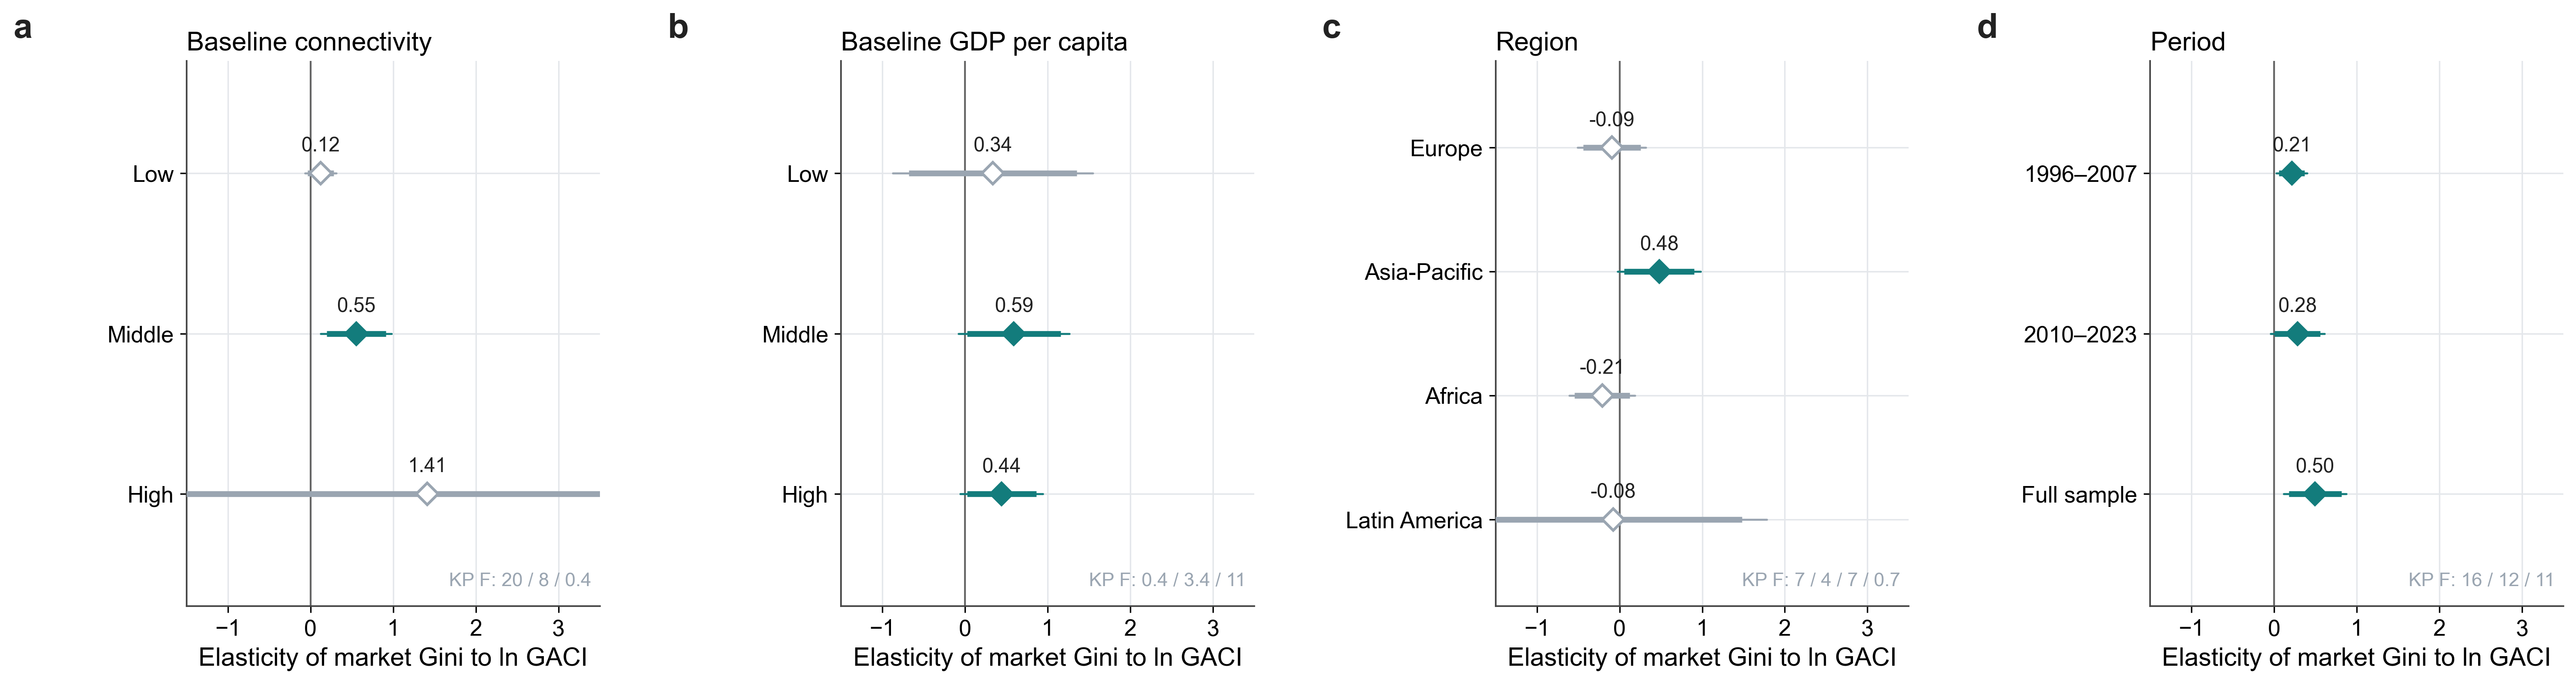
\includegraphics[width=\linewidth]{figures/Fig2_heterogeneity_v2.png}
\caption{Heterogeneity of the market-Gini elasticity to hub connectivity (2SLS on subsamples). (a) Terciles of $\mathrm{GACI}_{max}$ in 1996. (b) Terciles of baseline GDP per capita. (c) Macro region. (d) Era. Diamonds are point estimates; thick bars are 90 percent and thin bars 95 percent confidence intervals. Hollow markers denote estimates with $p\ge 0.10$; the first-stage KP $F$ of each subsample is reported in Table~\ref{tab:growth_ineq} and Appendix Tables~\ref{tab:a_stage} and \ref{tab:a_regions}.}
\label{fig:heterogeneity}
\end{figure}

The first-stage column disciplines what can be read. The instrument has power among the smaller hubs, with $F$ of $22.2$ below the median, $19.7$ and $8.1$ in the low and middle terciles, and $20.3$ and $7.5$ in the first two quartiles of Appendix Table~\ref{tab:a_stagedefs}, and none among the larger hubs ($F$ below one in the upper half, the top tercile and the top two quartiles). This is a substantive fact rather than a nuisance: the global expansion of aviation moved the connectivity of hubs that were joining the network, not of the hubs that already anchored it, so the estimates describe hubs in their integrating phase. Within that phase the picture is clear. Below the median, a one percent increase in hub connectivity raises GDP per capita by $1.22$ percent and WID mean income by $1.32$ percent ($p<0.01$), and at the same time raises the market Gini by $0.356$ percent and the disposable Gini by $0.399$ percent (both $p<0.01$). The same countries in which the hub raises income are the countries in which it raises inequality.

The terciles show that the two responses do not arrive at the same moment. In the lowest tercile, where the hub is smallest, connectivity raises GDP per capita and mean income with elasticities of $1.7$ and $1.5$ ($p<0.01$) and does not raise the Gini ($0.122$, standard error $0.096$); Appendix Table~\ref{tab:a_stage} shows that in this group the bottom half's income rises by as much as the mean ($1.727$, $p<0.01$) and its share does not fall. In the middle tercile, where the hub is integrating from a moderate base, the growth response is smaller ($0.891$, $p<0.10$) and the inequality response is at its largest ($0.554$, $p<0.05$), with the bottom-half share falling by about one percent for each percent of connectivity ($-1.011$, $p<0.01$). The quartiles of Appendix Table~\ref{tab:a_stagedefs} sharpen the contrast: the smallest quartile has a GDP elasticity of $1.702$ and a Gini elasticity of $0.074$, the second quartile a GDP elasticity of $0.728$ and a Gini elasticity of $0.720$ ($p<0.01$). The sequence is the one the sorting mechanism implies: when a country first acquires international connectivity the gain is broad, and as the hub becomes a gateway the gain concentrates in the hub economy. Appendix Tables~\ref{tab:a_stagedefs} and \ref{tab:a_stagedefs2} show that this pattern is not specific to the 1996 tercile definition; wherever the instrument has power, under alternative base years, cut points and connectivity measures, the distributional pattern is the same. Panel (b) of Figure~\ref{fig:heterogeneity} shows the same by baseline income: the elasticity is positive in the middle and high GDP terciles ($0.591$ and $0.443$, $p<0.10$) and the instrument has no power in the lowest income tercile. Panel (d) shows that the effect is present in both the 1996--2007 and the 2010--2023 eras ($0.214$ and $0.282$, $p<0.05$ and $p<0.10$), so it is not a feature of one aviation cycle. These results bear on \textbf{Hypothesis~4}, which predicts the largest effect in economies whose hubs are integrating from a small base, and support it.

%=======================================================================
\subsection{Mechanism: the hub, not the network; the distribution, not growth}
\label{sec:mechanism}
We now ask five questions about how hub connectivity raises inequality, each answered by a table. Together they describe a single chain: the effect is carried by the hub rather than by the network (I); it takes the form of the upper half rising with the mean while the bottom half is bypassed (II); it is not a growth effect (III); it is found where a hub economy exists to absorb the gains and it does not cross borders (IV); and it is not offset by redistribution (V).

\paragraph{(I) Which connectivity carries the effect?}
Table~\ref{tab:mech_A} separates the hub from the network. Column (1) repeats the baseline. Column (2) adds total connectivity as a control: the coefficient on instrumented hub connectivity rises to $0.756$ ($p<0.05$) while total connectivity, which now measures the network net of the hub, enters at $-0.105$ ($p<0.10$). Column (3) replaces the sum by the connectivity of the country's secondary airports and gives the same picture ($0.764$ on the hub, $-0.067$ on the secondaries, the latter imprecise). Holding the network fixed, the hub is disequalising and the rest of the network is, if anything, equalising: a country whose connectivity grows through its secondary cities does not experience the widening that a country whose connectivity grows through its gateway does. Columns (4) and (5) look inside the hub. Instrumenting the hub's eigenvector centrality, its integration with the global core of the network, and controlling for its seat capacity gives $0.133$ on centrality ($p<0.05$) and $-0.165$ on capacity ($p<0.05$); instrumenting capacity and controlling for flow betweenness gives $0.089$ on capacity ($p<0.01$) and $-0.011$ on betweenness. Appendix Table~\ref{tab:a_components} reports every component one at a time and the full set of horse races; because a single shifter moves every component, the one-at-a-time estimates are not separately identified, and the horse races are the informative comparison. In them, integration with the core wins over volume, and volume wins over transit. Column (6) confirms the composition result in OLS: with total connectivity held fixed, a more concentrated airport network, measured by the Herfindahl index of airport shares, is associated with a higher Gini ($0.087$, $p<0.01$). These results bear on the first part of \textbf{Hypothesis~3}, that the effect is specific to the hub, and support it.

\begin{table}[H]
\centering
\caption{Mechanism (I): which connectivity carries the effect?}
\label{tab:mech_A}
\begin{minipage}{\linewidth}
\centering
\resizebox{\linewidth}{!}{%
\begin{tabular}{lcccccc}
\toprule
\midrule
\multicolumn{7}{l}{\emph{Panel A. Which connectivity? Dependent variable: ln market Gini}}\\
 & (1) & (2) & (3) & (4) & (5) & (6) \\
 & Baseline & Hub + network & Hub + secondary & Core integration & Capacity + transit & Concentration (OLS) \\
\midrule
$\ln\mathrm{GACI}_{max}$ (hub), instrumented & 0.495\sym{**} & 0.756\sym{**} & 0.764\sym{*} &  &  &  \\
 & (0.194) & (0.351) & (0.442) &  &  &  \\
$\ln\mathrm{GACI}_{sum}$ (whole network), control &  & -0.105\sym{*} &  &  &  &  \\
 &  & (0.054) &  &  &  &  \\
ln GACI of secondary airports, control &  &  & -0.067 &  &  &  \\
 &  &  & (0.043) &  &  &  \\
ln hub eigenvector centrality, instrumented &  &  &  & 0.133\sym{**} &  &  \\
 &  &  &  & (0.053) &  &  \\
ln hub seat capacity &  &  &  & -0.165\sym{**} & 0.089\sym{***} &  \\
 &  &  &  & (0.072) & (0.030) &  \\
ln hub flow betweenness, control &  &  &  &  & -0.011\sym{*} &  \\
 &  &  &  &  & (0.007) &  \\
ln Herfindahl of airport shares (with $\ln\mathrm{GACI}_{sum}$) &  &  &  &  &  & 0.087\sym{***} \\
 &  &  &  &  &  & (0.026) \\
KP $F$ & 10.6 & 5.9 & 3.8 & 22.2 & 26.9 &  \\
Observations & 3{,}735 & 3{,}735 & 3{,}134 & 3{,}735 & 3{,}735 & 3{,}735 \\
\bottomrule
\end{tabular}}
\par\vspace{3pt}\begin{flushleft}\footnotesize Column (4) instruments the hub's eigenvector centrality and controls for its seat capacity; column (5) instruments seat capacity and controls for flow betweenness; column (6) is OLS. Country-year panel, 1996--2023. All regressions include country and year fixed effects and log population. 2SLS instruments ln GACI with the Feyrer interaction $Z_{ct}=a_t\times\ln \mathrm{MA}^{air}_{c,1996}$. Standard errors clustered by country in parentheses. \sym{*}~$p<0.10$, \sym{**}~$p<0.05$, \sym{***}~$p<0.01$.\end{flushleft}
\end{minipage}
\end{table}


\paragraph{(II) Who gains?}
Table~\ref{tab:mech_B} collects the incidence results in one row. Mean income rises ($1.219$), the seventh decile rises ($1.052$), the top decile rises by more ($1.443$), the bottom half does not rise ($0.445$, standard error $0.593$) and its share falls ($-0.774$). The two ratios locate the widening: the distance between the median and the bottom decile rises ($2.260$, $p<0.05$) and the distance between the top decile and the median does not ($0.747$, standard error $0.485$). The gap opens below the median, not above it.

\begin{table}[H]
\centering
\caption{Mechanism (II): who gains? Group incomes and ratios (2SLS).}
\label{tab:mech_B}
\begin{minipage}{\linewidth}
\centering
\resizebox{\linewidth}{!}{%
\begin{tabular}{lccccccc}
\toprule
\midrule
 & Mean income & p60--70 & p90--100 & Bottom-50 income & Bottom-50 share & p50/p10 & p90/p50 \\
\midrule
$\ln\mathrm{GACI}_{max}$, instrumented & 1.219\sym{**} & 1.052\sym{*} & 1.443\sym{***} & 0.445 & -0.774\sym{*} & 2.260\sym{**} & 0.747 \\
 & (0.491) & (0.546) & (0.513) & (0.593) & (0.417) & (0.916) & (0.485) \\
KP $F$ & 10.5 & 10.5 & 10.5 & 10.5 & 10.5 & 10.5 & 10.5 \\
Observations & 3{,}714 & 3{,}714 & 3{,}714 & 3{,}714 & 3{,}714 & 3{,}716 & 3{,}716 \\
\bottomrule
\end{tabular}}
\par\vspace{3pt}\begin{flushleft}\footnotesize Outcomes in logs: average pretax income of the group, its income share (identity-based), and ratios of decile mean incomes. Country-year panel, 1996--2023. All regressions include country and year fixed effects and log population. 2SLS instruments ln GACI with the Feyrer interaction $Z_{ct}=a_t\times\ln \mathrm{MA}^{air}_{c,1996}$. Standard errors clustered by country in parentheses. \sym{*}~$p<0.10$, \sym{**}~$p<0.05$, \sym{***}~$p<0.01$.\end{flushleft}
\end{minipage}
\end{table}


\paragraph{(III) Not a growth effect}
Connectivity raises GDP per capita with an elasticity of $1.294$ ($p<0.01$; the $a$-path of Equation~\eqref{eq:mec1}). If the inequality response were a by-product of this growth, holding GDP per capita fixed would remove it. Table~\ref{tab:mech_C} shows that it does the opposite: with GDP per capita as a control, the coefficient on instrumented hub connectivity rises from $0.495$ to $0.753$ ($p<0.05$), and GDP per capita itself enters at $-0.199$ ($p<0.05$). Growth is equalising in these data; the disequalising effect of the hub is what remains after the growth it generates is netted out, and it is larger than the total. Appendix Table~\ref{tab:a_mediators} applies the same decomposition to eighteen candidate mediators. Connectivity moves many of them in the direction the aviation literature predicts: international tourist arrivals ($a=3.90$), industrial employment ($18.7$ points), trade relative to GDP ($109$ points), differentiated-goods trade ($2.97$), high value-to-weight trade ($2.66$) and the number of export partners ($1.94$) all rise, and agricultural employment and resource rents fall. But every mediator that responds to connectivity is associated with a lower Gini, so in every row the conditional coefficient $c'$ exceeds the baseline. The structural changes that connectivity induces, industrialisation, trade diversification and the shift toward differentiated exports, are the equalising forces; the widening is not carried by any of them. This bears on the second part of \textbf{Hypothesis~3}, that the effect is not carried by growth, and supports it.

\begin{table}[H]
\centering
\caption{Mechanism (III): not a growth effect.}
\label{tab:mech_C}
\begin{threeparttable}
\small
\begin{tabular}{lc}
\toprule
\midrule
 & ln market Gini \\
\midrule
$\ln\mathrm{GACI}_{max}$, instrumented (direct effect $c'$) & 0.753\sym{**} \\
 & (0.325) \\
ln GDP per capita, control ($b$) & -0.199\sym{**} \\
 & (0.087) \\
Memo: hub $\rightarrow$ ln GDP per capita, 2SLS ($a$) & 1.294\sym{***} \\
 & (0.428) \\
KP $F$ & 6.5 \\
Observations & 3{,}735 \\
\bottomrule
\end{tabular}
\begin{tablenotes}\small
\item GDP per capita is itself an outcome of connectivity ($a$-path), so it is not a valid control in the baseline; holding it fixed isolates the distributional effect from the growth effect. Other candidate mediators are reported in Appendix Table~\ref{tab:a_mediators}. Country-year panel, 1996--2023. All regressions include country and year fixed effects and log population. 2SLS instruments ln GACI with the Feyrer interaction $Z_{ct}=a_t\times\ln \mathrm{MA}^{air}_{c,1996}$. Standard errors clustered by country in parentheses. \sym{*}~$p<0.10$, \sym{**}~$p<0.05$, \sym{***}~$p<0.01$.
\end{tablenotes}
\end{threeparttable}
\end{table}


\paragraph{(IV) Where is the effect found?}
Table~\ref{tab:mech_D} splits the sample along the dimensions the sorting mechanism singles out. The effect is present in economies whose urbanisation is above the median ($0.690$, $p<0.05$) and absent below it ($0.234$, standard error $0.225$): a hub widens the distribution where there is an urban economy for the hub to concentrate. It is present in economies that are not tourism-dependent ($0.425$, $p<0.01$), which rules out tourism employment as the carrier and is consistent with business rather than leisure travel as the relevant traffic. It is absent in the lowest tercile of baseline hub size ($0.122$) and present in the middle tercile ($0.554$, $p<0.05$), the take-off stage identified in Section~\ref{sec:growthineq}, and it is imprecise in economies above the median of trade openness ($0.222$), where the hub is one of several channels of integration. The last column enters own connectivity together with the leave-out mean of contiguous neighbours' connectivity, each instrumented by its own shifter: the own effect is $0.567$ ($p<0.05$) and the neighbours' is $-0.099$ (standard error $0.135$). Appendix Table~\ref{tab:a_spill} repeats the exercise for neighbours within 500 km, the five nearest neighbours and neighbours-only specifications, with the same result: a neighbouring country's hub does not widen the domestic distribution. The effect is a property of the country's own gateway.

\begin{table}[H]
\centering
\caption{Mechanism (IV): where is the effect found? Split samples and neighbours (ln market Gini).}
\label{tab:mech_D}
\begin{minipage}{\linewidth}
\centering
\resizebox{\linewidth}{!}{%
\begin{tabular}{lccccccc}
\toprule
\midrule
 & Urban. above & Urban. below & Non-tourism & Thin networks & Take-off hubs & Open economies & Own + neighbours \\
\midrule
$\ln\mathrm{GACI}_{max}$, instrumented & 0.690\sym{**} & 0.234 & 0.425\sym{***} & 0.122 & 0.554\sym{**} & 0.222 & 0.567\sym{**} \\
 & (0.289) & (0.225) & (0.147) & (0.096) & (0.219) & (0.149) & (0.227) \\
Neighbours' ln GACI (contiguity), instrumented &  &  &  &  &  &  & -0.099 \\
 &  &  &  &  &  &  & (0.135) \\
KP $F$ & 7.9 & 4.3 & 8.8 & 19.7 & 8.1 & 12.2 & 4.0 \\
Observations & 1{,}960 & 1{,}775 & 1{,}774 & 1{,}048 & 1{,}310 & 1{,}650 & 3{,}735 \\
\bottomrule
\end{tabular}}
\par\vspace{3pt}\begin{flushleft}\footnotesize Splits at the median of the earliest observed value (urbanisation, trade to GDP, tourism receipts as a share of exports) or at terciles of $\mathrm{GACI}_{max}$ in 1996 (thin networks: lowest tercile; take-off hubs: middle tercile). The last column instruments own connectivity with the own shifter and the leave-out mean of contiguous neighbours' ln GACI with their shifters. Country-year panel, 1996--2023. All regressions include country and year fixed effects and log population. 2SLS instruments ln GACI with the Feyrer interaction $Z_{ct}=a_t\times\ln \mathrm{MA}^{air}_{c,1996}$. Standard errors clustered by country in parentheses. \sym{*}~$p<0.10$, \sym{**}~$p<0.05$, \sym{***}~$p<0.01$.\end{flushleft}
\end{minipage}
\end{table}


\paragraph{(V) Is the effect offset by redistribution?}
Finally, Table~\ref{tab:mech_E} asks whether taxes and transfers offset the market response. They do not. The disposable-income Gini rises by more than the market Gini ($0.651$ against $0.495$), the redistribution wedge, market minus disposable Gini in points, falls by $6.0$ points for a unit increase in log connectivity ($p<0.10$), and its log ratio falls ($-0.156$, $p<0.10$). Tax revenue relative to GDP does not respond (the instrument is weak in the smaller tax sample). Redistribution in the economies whose hubs are integrating therefore did not expand to meet the widening of the market distribution; if anything it contracted, which is the pattern the evidence on globalisation and the tax burden would predict \citep{Egger_2019,Kleven_2013}. This completes the test of \textbf{Hypothesis~4}: the effect is concentrated in urbanised, non-tourism economies with hubs in their integrating phase, it does not cross borders, and it is not offset by redistribution.

\begin{table}[H]
\centering
\caption{Mechanism (V): is the effect offset by redistribution?}
\label{tab:mech_E}
\begin{minipage}{\linewidth}
\centering
\resizebox{\linewidth}{!}{%
\begin{tabular}{lcccc}
\toprule
\midrule
 & ln disposable Gini & Market $-$ disposable Gini (points) & ln(market/disposable Gini) & Tax revenue, \% GDP \\
\midrule
$\ln\mathrm{GACI}_{max}$, instrumented & 0.651\sym{***} & -6.010\sym{*} & -0.156\sym{*} & -3.589 \\
 & (0.241) & (3.607) & (0.086) & (11.492) \\
KP $F$ & 10.6 & 10.6 & 10.6 & 4.8 \\
Observations & 3{,}735 & 3{,}735 & 3{,}735 & 2{,}595 \\
\bottomrule
\end{tabular}}
\par\vspace{3pt}\begin{flushleft}\footnotesize The wedge is the redistribution achieved by taxes and transfers; a negative coefficient means less redistribution. Country-year panel, 1996--2023. All regressions include country and year fixed effects and log population. 2SLS instruments ln GACI with the Feyrer interaction $Z_{ct}=a_t\times\ln \mathrm{MA}^{air}_{c,1996}$. Standard errors clustered by country in parentheses. \sym{*}~$p<0.10$, \sym{**}~$p<0.05$, \sym{***}~$p<0.01$.\end{flushleft}
\end{minipage}
\end{table}


%=======================================================================
\subsection{Robustness}
\label{sec:robust}
Table~\ref{tab:robust} probes the headline estimate along three dimensions. Panel B varies the sample: excluding the ten largest hub economies gives $0.565$ ($p<0.01$), restricting the sample to 1996--2019 gives $0.439$ ($p<0.01$), and excluding the financial-crisis and pandemic years gives $0.480$ ($p<0.05$), each with a similar first stage. The estimate is not driven by the world's largest gateways or by the crisis episodes in which connectivity collapsed. Panel C addresses the identifying assumption directly. Because a shift-share instrument with a single shifter is valid only if the exposure is unrelated to other trends, we allow five other baseline characteristics, GDP per capita, the market Gini, land area, absolute latitude and sea market access, each to have its own trend in the aviation index. The estimate falls to $0.377$ for the market Gini and $0.506$ for the disposable Gini (both $p<0.05$) with an unchanged first stage; the result is not an artefact of baseline income, baseline inequality or general geography trending with the aviation cycle, although its magnitude falls by about a quarter once other exposures are allowed their own trends. Panel D holds the point estimate fixed and varies the variance estimator. Clustering by country gives a standard error of $0.198$, two-way clustering by country and year $0.190$, and Conley spatial HAC with 1{,}000 and 2{,}000 km cutoffs $0.203$ and $0.224$ \citep{Conley_1999}; the market-Gini estimate remains significant at 5 percent under every estimator and the disposable-Gini estimate at 1 or 5 percent. Spatial correlation between neighbouring countries does not account for the precision.

\begin{table}[H]
\centering
\caption{Robustness of the headline estimate: sample, fixed effects and inference (2SLS, Feyrer instrument).}
\label{tab:robust}
\begin{threeparttable}
\small
\begin{tabular}{lcccc}
\toprule
 & ln market Gini & ln disposable Gini & KP $F$ & N \\
\midrule
\multicolumn{5}{l}{\emph{Panel A. Baseline}}\\
2SLS, Feyrer instrument (Table~\ref{tab:main}) & 0.495\sym{**} & 0.651\sym{***} & 10.6 & 3{,}735 \\
 & (0.194) & (0.241) \\
\multicolumn{5}{l}{\emph{Panel B. Sample}}\\
Excluding the ten largest hub economies & 0.565\sym{***} & 0.709\sym{***} & 9.9 & 3{,}472 \\
 & (0.204) & (0.254) \\
1996--2019 & 0.439\sym{***} & 0.574\sym{***} & 12.6 & 3{,}344 \\
 & (0.163) & (0.200) \\
Excluding 2008--09 and 2020--21 & 0.480\sym{**} & 0.635\sym{***} & 11.3 & 3{,}204 \\
 & (0.188) & (0.233) \\
\multicolumn{5}{l}{\emph{Panel C. Exposure trends}}\\
Baseline exposures $\times$ aviation index & 0.377\sym{**} & 0.506\sym{**} & 9.9 & 3{,}735 \\
 & (0.187) & (0.229) \\
\multicolumn{5}{l}{\emph{Panel D. Inference (same point estimates as the baseline)}}\\
Clustered by country & 0.495\sym{**} & 0.651\sym{***} & 10.7 & 3{,}737 \\
 & (0.198) & (0.247) \\
Two-way clustered (country, year) & 0.495\sym{***} & 0.651\sym{***} & 10.7 & 3{,}737 \\
 & (0.190) & (0.238) \\
Conley spatial HAC, 1{,}000 km & 0.495\sym{**} & 0.651\sym{***} & 10.7 & 3{,}737 \\
 & (0.203) & (0.248) \\
Conley spatial HAC, 2{,}000 km & 0.495\sym{**} & 0.651\sym{**} & 10.7 & 3{,}737 \\
 & (0.224) & (0.267) \\
\bottomrule
\end{tabular}
\begin{tablenotes}\small
\item Panel D re-estimates the baseline with alternative variance estimators; Conley standard errors use a Bartlett kernel in great-circle distance between country centroids with the stated cutoff and allow arbitrary within-country serial correlation. Baseline exposures are ln GDP per capita, the market Gini, ln land area, absolute latitude and ln sea market access in the base year, each interacted with the aviation index. Country-year panel, 1996--2023. All regressions include country and year fixed effects and log population. 2SLS instruments ln GACI with the Feyrer interaction $Z_{ct}=a_t\times\ln \mathrm{MA}^{air}_{c,1996}$. Standard errors clustered by country in parentheses. \sym{*}~$p<0.10$, \sym{**}~$p<0.05$, \sym{***}~$p<0.01$.
\end{tablenotes}
\end{threeparttable}
\end{table}


Table~\ref{tab:measures} varies the measurement of both sides of the regression. Across the three connectivity aggregations (panels) and six inequality measures (columns), every 2SLS coefficient is positive. The SWIID market and disposable Gini, the Palma ratio, the ratio of top- to bottom-decile mean income and the absolute gap between top-decile and bottom-half incomes are all significant for hub connectivity ($0.495$, $0.651$, $1.202$, $2.456$ and $1.504$), and the same holds for hub quality and total connectivity. The Gini computed from the WID deciles alone is positive but imprecise ($0.218$, standard error $0.161$), which reflects the coarser ten-group construction. The result is a property of the distribution, not of one summary of it or of one aggregation of connectivity. Appendix Table~\ref{tab:a_lags} shows that the estimate is stable when connectivity is lagged: the coefficient on hub connectivity lagged one to ten years lies between $0.40$ and $0.52$ and remains significant at every horizon, so the widening is persistent rather than a contemporaneous fluctuation.

\begin{table}[H]
\centering
\caption{Robustness to the connectivity measure and to the inequality measure.}
\label{tab:measures}
\begin{threeparttable}
\small
\begin{tabular}{lcccccc}
\toprule
 & SWIID market Gini & SWIID disp. Gini & WID Gini & Palma ratio & p90/p10 & Absolute gap \\
\midrule
\multicolumn{7}{l}{\emph{Panel A. Hub connectivity, $\ln\mathrm{GACI}_{max}$}}\\
OLS & 0.061\sym{***} & 0.050\sym{*} & 0.060\sym{*} & 0.152 & 0.329\sym{**} & 0.766\sym{***} \\
 & (0.023) & (0.026) & (0.033) & (0.095) & (0.134) & (0.116) \\
2SLS & 0.495\sym{**} & 0.651\sym{***} & 0.218 & 1.202\sym{*} & 2.456\sym{**} & 1.504\sym{***} \\
 & (0.194) & (0.241) & (0.161) & (0.681) & (1.148) & (0.528) \\
KP $F$ (2SLS) & 10.6 & 10.6 & 10.5 & 10.5 & 13.5 & 10.5 \\
Observations & 3{,}735 & 3{,}735 & 3{,}714 & 3{,}714 & 3{,}443 & 3{,}714 \\
\addlinespace
\multicolumn{7}{l}{\emph{Panel B. Hub quality, $\ln\mathrm{GACI}_{cwm}$}}\\
OLS & 0.079\sym{***} & 0.060\sym{**} & 0.046 & 0.098 & 0.240 & 0.787\sym{***} \\
 & (0.026) & (0.030) & (0.035) & (0.105) & (0.155) & (0.129) \\
2SLS & 0.595\sym{**} & 0.783\sym{***} & 0.261 & 1.441\sym{*} & 2.968\sym{**} & 1.804\sym{***} \\
 & (0.240) & (0.302) & (0.192) & (0.827) & (1.435) & (0.652) \\
KP $F$ (2SLS) & 8.8 & 8.8 & 8.7 & 8.7 & 11.0 & 8.7 \\
Observations & 3{,}735 & 3{,}735 & 3{,}714 & 3{,}714 & 3{,}443 & 3{,}714 \\
\addlinespace
\multicolumn{7}{l}{\emph{Panel C. Total connectivity, $\ln\mathrm{GACI}_{sum}$}}\\
OLS & 0.008 & 0.009 & 0.005 & 0.014 & 0.074 & 0.181\sym{***} \\
 & (0.007) & (0.009) & (0.008) & (0.027) & (0.051) & (0.038) \\
2SLS & 0.199\sym{***} & 0.262\sym{***} & 0.089 & 0.490\sym{*} & 1.016\sym{**} & 0.614\sym{***} \\
 & (0.077) & (0.090) & (0.065) & (0.264) & (0.450) & (0.219) \\
KP $F$ (2SLS) & 18.0 & 18.0 & 17.4 & 17.4 & 21.3 & 17.4 \\
Observations & 3{,}735 & 3{,}735 & 3{,}714 & 3{,}714 & 3{,}443 & 3{,}714 \\
\addlinespace
\bottomrule
\end{tabular}
\begin{tablenotes}\small
\item Outcomes in logs. SWIID Gini indices are household-equivalised survey-based series \citep{Solt_2020}. WID measures are computed from the pretax national income shares of ten deciles (equal-split adults): the WID Gini is the DINA Gini; Palma $=$ top-10 share / bottom-40 share; p90/p10 is the ratio of top- to bottom-decile mean income; the absolute gap is the top-10 minus bottom-50 average income in constant local prices. Country-year panel, 1996--2023. All regressions include country and year fixed effects and log population. 2SLS instruments ln GACI with the Feyrer interaction $Z_{ct}=a_t\times\ln \mathrm{MA}^{air}_{c,1996}$. Standard errors clustered by country in parentheses. \sym{*}~$p<0.10$, \sym{**}~$p<0.05$, \sym{***}~$p<0.01$.
\end{tablenotes}
\end{threeparttable}
\end{table}


%=======================================================================
\subsection{Aggregate contribution of connectivity growth, 1996--2023}
\label{sec:aggregate}
How much of the change in within-country inequality over the sample period do the estimates attribute to hub connectivity? For each of the 138 countries with at least fifteen years of complete data, we multiply the observed change in $\ln\mathrm{GACI}_{max}$ between the first and last year by the 2SLS elasticities: the Gini elasticity of Table~\ref{tab:main} and the group income and share elasticities of Table~\ref{tab:incidence}, the latter converted to share points using each country's initial share. Figure~\ref{fig:attribution} maps the implied change in the market Gini and in the bottom-half share and ranks the countries with the largest implied changes; Appendix Table~\ref{tab:a_aggregate} reports regional and world aggregates against the observed changes.

\begin{figure}[H]
\centering
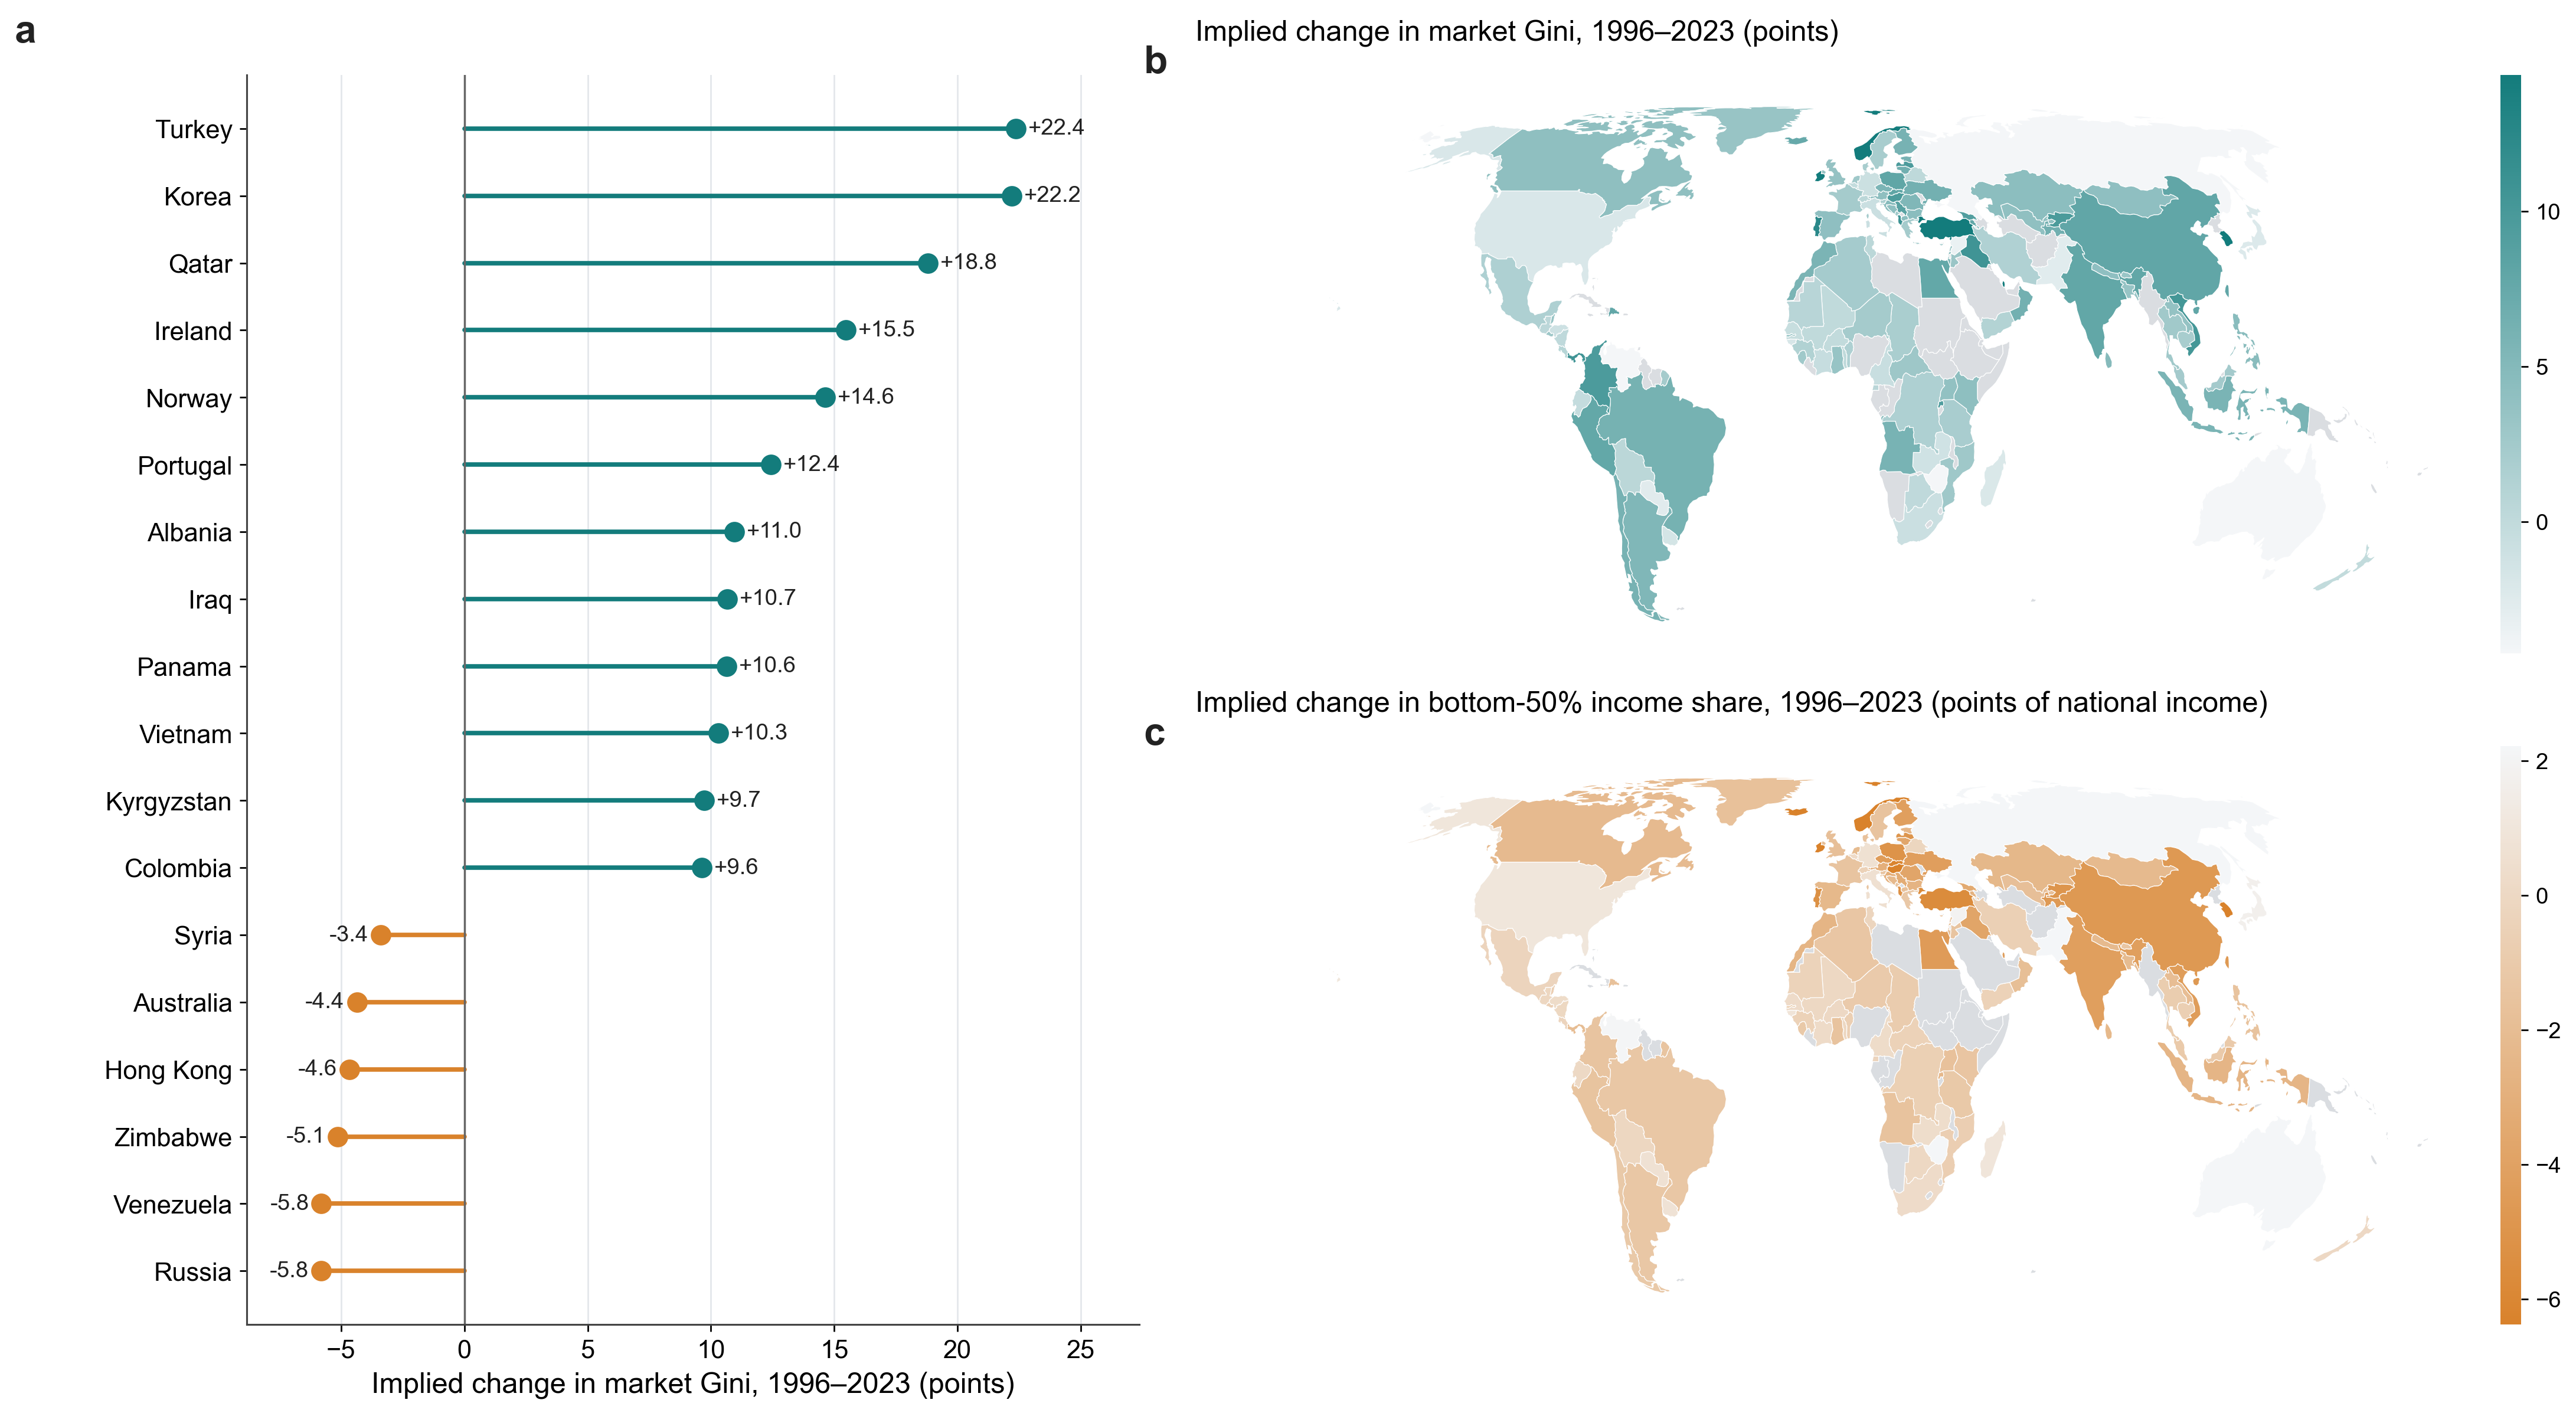
\includegraphics[width=\linewidth]{figures/Fig3_attribution_v2.png}
\caption{Implied incidence of observed hub-connectivity growth, 1996--2023. (a) Countries with the largest implied increases and decreases in the market Gini, in points, from the observed change in $\ln\mathrm{GACI}_{max}$ multiplied by the 2SLS elasticity of Table~\ref{tab:main}. (b) Implied change in the market Gini by country. (c) Implied change in the bottom-half share of pretax national income, in points of national income, from the share elasticity of Table~\ref{tab:incidence}. Grey denotes countries with fewer than fifteen years of complete data.}
\label{fig:attribution}
\end{figure}

Hub connectivity rose in 80 percent of the 138 countries, by $0.15$ log points on average and by $0.21$ when countries are weighted by population. Applied to the elasticities, this growth implies an increase of $3.6$ Gini points for the unweighted average country and $5.0$ points for the population-weighted world, and a decline of $1.6$ and $2.4$ points of national income in the bottom-half share. The largest implied increases are in the economies whose hubs became global gateways over the period: Turkey and Korea ($22$ points each, from roughly a doubling of hub connectivity), Qatar ($19$), Ireland ($15$) and Norway ($15$); the implied changes are negative where hub connectivity fell, as in Russia, Venezuela and Hong Kong. By region, the implied increase is largest in Europe and Asia-Pacific ($5.5$ and $4.8$ points) and smallest in Africa and Latin America ($1.7$ and $2.7$), where hubs grew less. Against these implied changes, the observed change in the population-weighted world market Gini was $+0.4$ points and in the bottom-half share $-2.1$ points. The comparison says two things. First, the bottom-half share moved over the period by about what connectivity growth alone would imply. Second, the Gini did not, which means that other forces, among them the growth, industrialisation and trade diversification that Section~\ref{sec:mechanism} shows to be equalising, offset most of the widening at the level of the summary index while the share of the bottom half still fell. As in the companion paper, this is a partial-equilibrium accounting that holds elasticities constant and abstracts from adjustment in prices, migration and policy; it is a statement of the order of magnitude the estimates imply, not a decomposition of history.

%=======================================================================
\subsection{Synthesis: the hypotheses revisited}
\label{sec:synthesis}
The results map onto the four hypotheses of Section~\ref{sec:framework} as follows. \textbf{Hypothesis~1}, that hub connectivity increases within-country inequality, is supported: instrumented hub connectivity raises the market Gini with an elasticity of $0.50$ and the disposable Gini with an elasticity of $0.65$ (Table~\ref{tab:main}), the pattern holds across all three aggregations of connectivity and across five inequality measures (Table~\ref{tab:measures}), and the estimate survives the sample, exposure-trend and inference checks of Table~\ref{tab:robust}. \textbf{Hypothesis~2}, that the response is located in the lower half of the distribution and not at the top percentile, is supported: from the seventh decile upward incomes rise with the mean, the bottom half does not rise and its share falls, the median-to-bottom ratio widens while the top-to-median ratio does not, and the top percentile does not gain relative to the top decile (Tables~\ref{tab:incidence} and \ref{tab:mech_B}). \textbf{Hypothesis~3}, that the effect is specific to the hub and not carried by growth, is supported: with the network held fixed the hub is disequalising and the network equalising, integration with the global core carries the effect within the hub, and holding GDP per capita or any of eighteen structural mediators fixed raises rather than lowers the estimate (Tables~\ref{tab:mech_A} and \ref{tab:mech_C}). \textbf{Hypothesis~4}, that the effect is concentrated in urbanised, non-tourism economies with hubs integrating from a small base, does not spill across borders and is not offset by redistribution, is supported (Tables~\ref{tab:growth_ineq}, \ref{tab:mech_D} and \ref{tab:mech_E}).

Read jointly, the four verdicts tell one story rather than four. Hub connectivity raises average income, and the same movement raises inequality, because the income arrives in the hub economy and is received by the upper half of the distribution that participates in it. The widening is not a side effect of growth, since growth itself equalises; it is not a property of connectivity in general, since a dispersed network equalises; and it is not a top-percentile phenomenon, since the very top does not pull away. It is the footprint of a gateway on the distribution of the country that possesses it, largest at the moment the gateway is forming, and it is not offset by the tax and transfer system. Taken together, these results carry three messages. First, the national income gain from hub connectivity is real but its incidence is not: the average return overstates the return to the lower half of the distribution, which does not participate. Second, the distributional cost is a consequence of the form connectivity growth takes, hub concentration, rather than of connectivity as such; the same connectivity distributed across secondary airports carries no such cost. Third, redistribution did not follow the hub, so the distributional outcome of hub development is a policy choice that governments made by default.

%=======================================================================
\section{Discussion}
\label{sec:discussion}
%=======================================================================
The central finding of this study is that the connectivity of a country's primary hub raises within-country income inequality, and that it does so by leaving the lower half of the distribution out of the growth it generates rather than by enriching the very top. The 2SLS estimate for hub connectivity implies an elasticity of the market Gini of $0.50$, and the incidence estimates show that the elasticity of mean income, $1.2$, is the average of an elasticity of about $1.1$ to $1.4$ for the upper half of the distribution and an elasticity indistinguishable from zero for the lower half. This is a stronger statement than the Gini alone conveys. A rise in the Gini could arise from many shapes of incidence; the decile estimates show that the shape here is a staircase with its step at the median, and that the top percentile moves with, not ahead of, the rest of the top decile. The result therefore does not describe a superstar economy. It describes an economy in which a broad upper segment, the households positioned to participate in the hub city's tradable-service and business economy, receives the return to the country's connectivity, while the households outside it grow at the rate they would have grown without it.

The mechanism analysis helps explain why this shape arises and where the evidence is stronger and weaker. Three findings support a sorting-and-agglomeration interpretation over the alternatives. First, the hub, not the network, carries the effect: with total connectivity or secondary-airport connectivity held fixed, hub connectivity remains disequalising and the rest of the network is equalising, and within the hub it is integration with the global core rather than volume or transit that matters. A dispersed network connects secondary cities to the world and spreads the connectivity-related activity across places; a gateway concentrates it. Second, the effect is not carried by growth or by any of the structural changes that connectivity induces. Connectivity raises GDP per capita, industrial employment, trade, differentiated-goods exports and export diversification, and every one of these is associated with lower inequality, so the disequalising effect is what remains after these equalising forces are netted out; it is larger than the total effect, which is why 2SLS exceeds OLS and why adding the mediators raises rather than lowers the estimate. Third, the effect appears where the sorting mechanism requires an urban economy and business rather than leisure traffic: in urbanised, non-tourism economies whose hubs are integrating from a moderate base. In the smallest hubs, where connectivity first arrives, the gain is broad and the bottom half rises with the mean; the concentration appears as the hub becomes a gateway. The mediation results should be interpreted as a descriptive decomposition rather than formal causal mediation, because each mediator is itself an outcome of connectivity, but their direction is uniform and it is the opposite of the direction the effect would need if it ran through them.

The redistribution result deserves emphasis because it is the margin on which policy operates. The disposable Gini rises by more than the market Gini, and the wedge between them narrows. Governments in the economies whose hubs integrated did not expand redistribution to meet the widening of the market distribution. One reading is the one the globalisation literature suggests: the gains accrue to mobile high earners and firms, the tax burden has shifted toward the middle, and the political economy of a gateway city favours investment in the gateway over transfers away from it \citep{Egger_2019,Kleven_2013}. Whatever the reason, the finding means that the distributional outcome of hub development is not an unavoidable consequence of connectivity; it is the joint outcome of a concentrated form of connectivity growth and a tax and transfer system that did not respond to it.

The heterogeneity results reconcile this paper with the companion finding that connectivity raises income most in the least developed economies. The two findings are not in tension; they are two moments of one process. When a country whose hub is small acquires international connectivity, the gain is large and broadly shared. As the hub grows into a gateway, the gain persists but concentrates in the hub economy, and inequality rises. The instrument identifies precisely these two phases, since the global expansion of aviation moved the connectivity of hubs that were integrating and not of the hubs that already anchored the network; the estimates are therefore most informative about hubs in the integrating phase and about connectivity changes of the kind the aviation cycle induces, and they say little about the marginal effect of connectivity at London, Frankfurt or Tokyo. A country deciding whether to develop a gateway is, however, in exactly the phase the estimates describe.

The aggregate accounting puts the magnitudes in perspective. Applied to observed connectivity growth, the elasticities imply a contribution of about five Gini points to population-weighted world within-country inequality over 1996--2023, and a decline of about two and a half points of national income in the bottom-half share, the latter close to the observed decline. Against a rise in the observed world Gini of less than half a point, this means that the equalising forces of the period, among them the growth, industrialisation and trade diversification that connectivity itself promoted, offset most of the widening at the level of the summary index, while the share of the bottom half still fell. The accounting is partial-equilibrium and holds elasticities constant, so it indicates orders of magnitude; but the order of magnitude is that hub development was one of the larger disequalising forces operating within countries over the period.

The policy implications follow. Airport and route investment and air-service liberalisation raise national income, and this paper does not qualify that conclusion. It qualifies its incidence. Where connectivity growth takes the form of a single gateway, the return accrues to the upper half of the distribution and the tax system, on the evidence here, does not redistribute it. Two policy margins follow from the mechanism. The first is the form of the network: because dispersed connectivity carries no distributional cost, the development of secondary international airports and of direct international service from second-tier cities is a way to obtain the income gain without the concentration, and the negative coefficient on network connectivity net of the hub suggests that it may narrow the distribution. The second is redistribution: the widening is concentrated in an identifiable phase of hub development and in identifiable economies, so a government that develops a gateway can anticipate it and respond with transfers, with investment in the connectivity of other regions, or with the spatial policies whose trade-offs \citet{Fajgelbaum_2020} analyse. The argument against doing nothing is that the default, on this evidence, is a wider distribution.

The study has limitations. First, the instrument identifies the effect of connectivity changes induced by the global aviation cycle in hubs that were integrating into the network; it has no power in the largest hubs and the estimates should not be extrapolated to them. Second, the mediation analysis is descriptive, as discussed above. Third, the SWIID Gini coefficients are harmonised estimates with model-based uncertainty that our standard errors do not incorporate, and the WID decile series combine survey, tax and national-accounts data whose quality varies across countries; the agreement between the two sources and across five inequality measures is reassuring but does not remove measurement error. Fourth, the aggregate accounting is partial equilibrium. Fifth, the heterogeneity splits have weaker first stages than the pooled sample and are correspondingly less precise, so the differences between groups are indicative rather than sharp. Extending the design to sub-national income data, so that the hub region and the rest of the country can be observed separately, and embedding the elasticities in a spatial equilibrium model in which migration, housing and wages adjust, are the natural next steps.

%=======================================================================
\section{Conclusion}
\label{sec:conclusion}
%=======================================================================
The evidence in this paper indicates that the connectivity of a country's primary hub raises within-country income inequality. Instrumenting a continuous, network-based connectivity index with a Feyrer-type interaction between the global aviation cycle and baseline geographic air market access, we estimate an elasticity of the market-income Gini of $0.50$ and of the disposable-income Gini of $0.65$, robust to the sample, to trends in other baseline exposures, to spatial and two-way clustered inference, to the aggregation of connectivity and to the measure of inequality. Decile-level estimates show how the effect works: the upper half of the distribution grows with mean income while the bottom half does not, so that the bottom half's share falls and the median pulls away from the bottom, whereas the top percentile does not pull away from the rest of the top. The effect is carried by the hub and not by the national network, by integration with the global core and not by traffic volume, and it is not a growth effect, since the growth and structural change that connectivity generates are themselves equalising. It is largest in urbanised, non-tourism economies whose hubs are integrating from a moderate base, it does not cross borders, and it is not offset by redistribution. Nearly three decades of hub-connectivity growth account for on the order of five Gini points of population-weighted world within-country inequality. Hub development raises average income and concentrates it in the same movement; the income gain from connectivity is real, and so is its incidence. The policy implication is that the form connectivity growth takes, and the redistribution that accompanies it, determine whether a country's gateway is a national asset or a metropolitan one.

%=======================================================================
\appendix
%=======================================================================
\section{Additional figures and tables}
\label{sec:appendix}
Figure~\ref{fig:evolution} describes the evolution of the global air network over the sample period and Figure~\ref{fig:mapchange} maps the change in hub connectivity that identifies the estimates.

\begin{figure}[H]
\centering
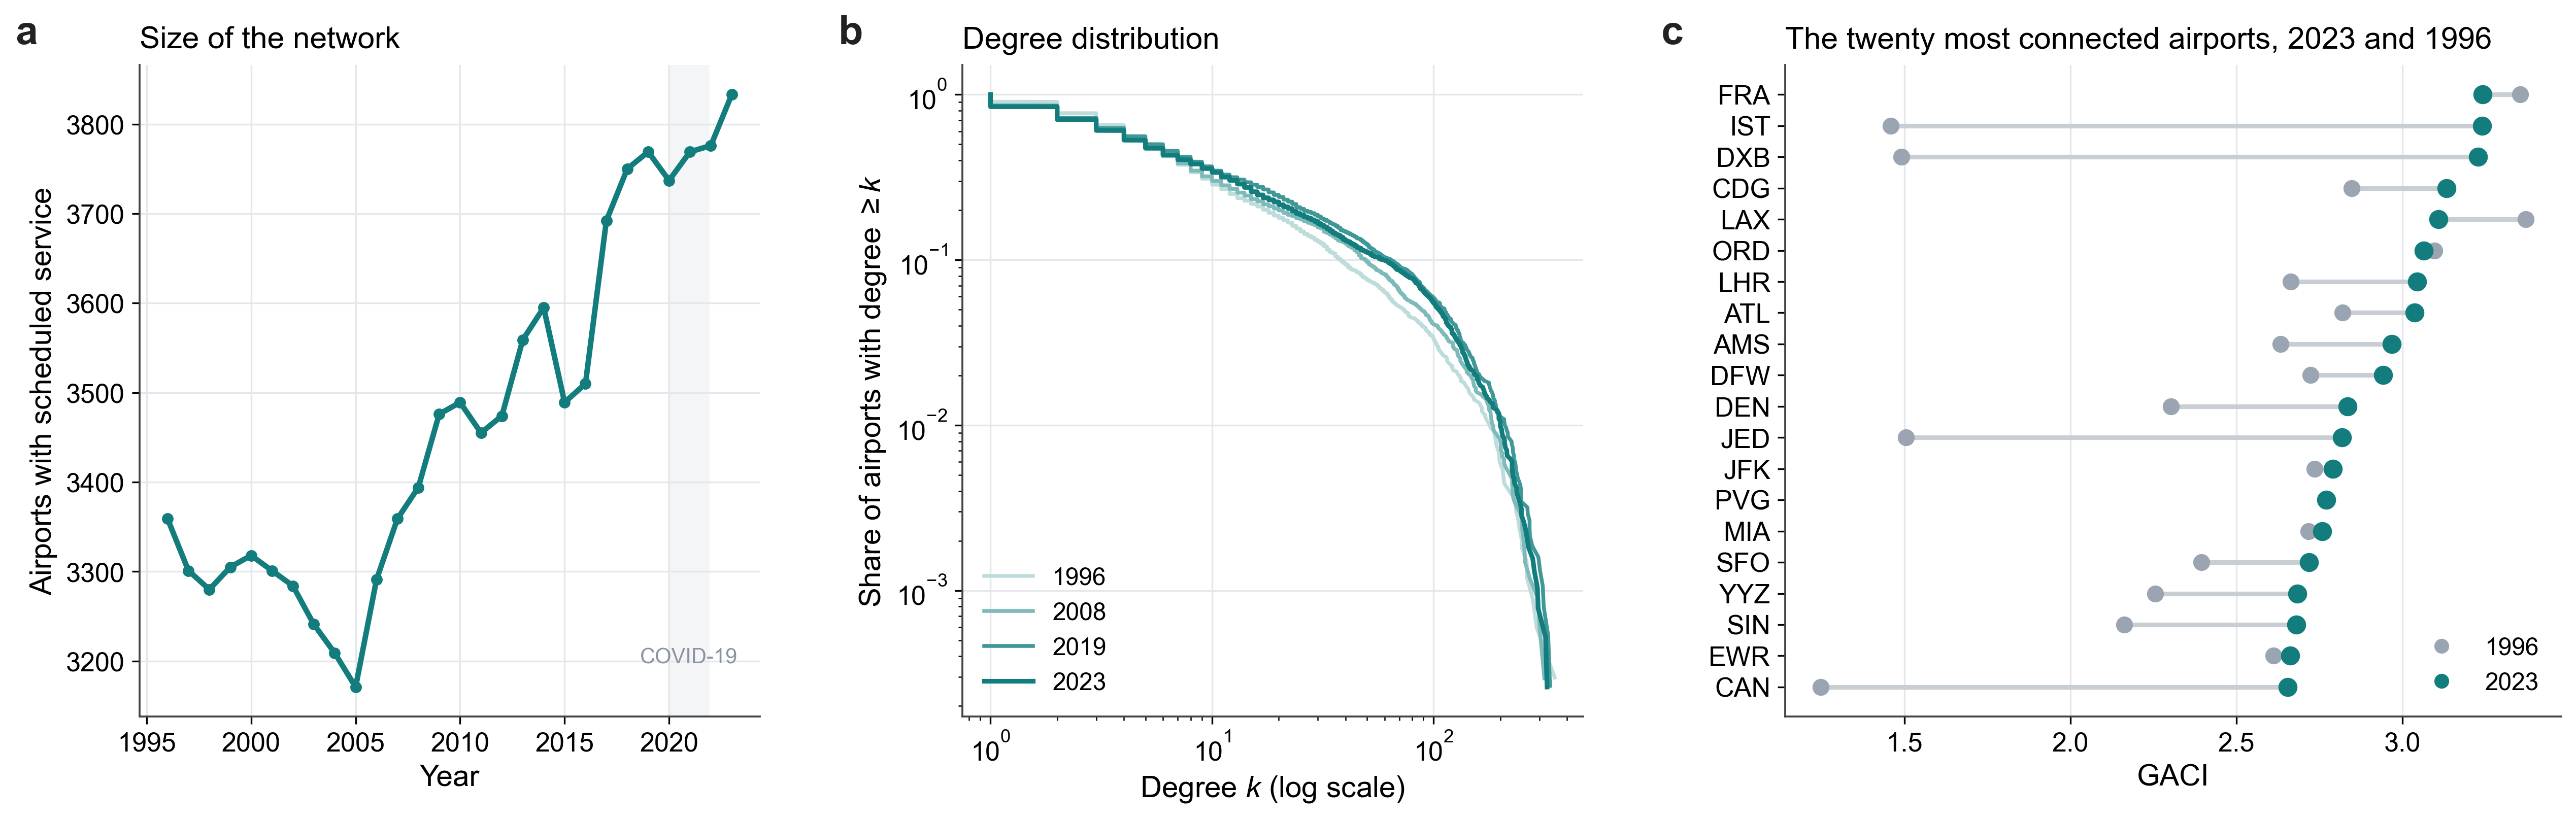
\includegraphics[width=\linewidth]{figures/FigB2_network_evolution.png}
\caption{Evolution of the global air network, 1996--2023. (a) Number of airports with scheduled service in each year's network. (b) Complementary cumulative distribution of degree (share of airports with at least $k$ direct connections) in 1996, 2008, 2019 and 2023, log scales. (c) The twenty airports with the highest GACI in 2023 (teal) and their index in 1996 (grey). Source: authors' airport-year panel.}
\label{fig:evolution}
\end{figure}

\begin{figure}[H]
\centering
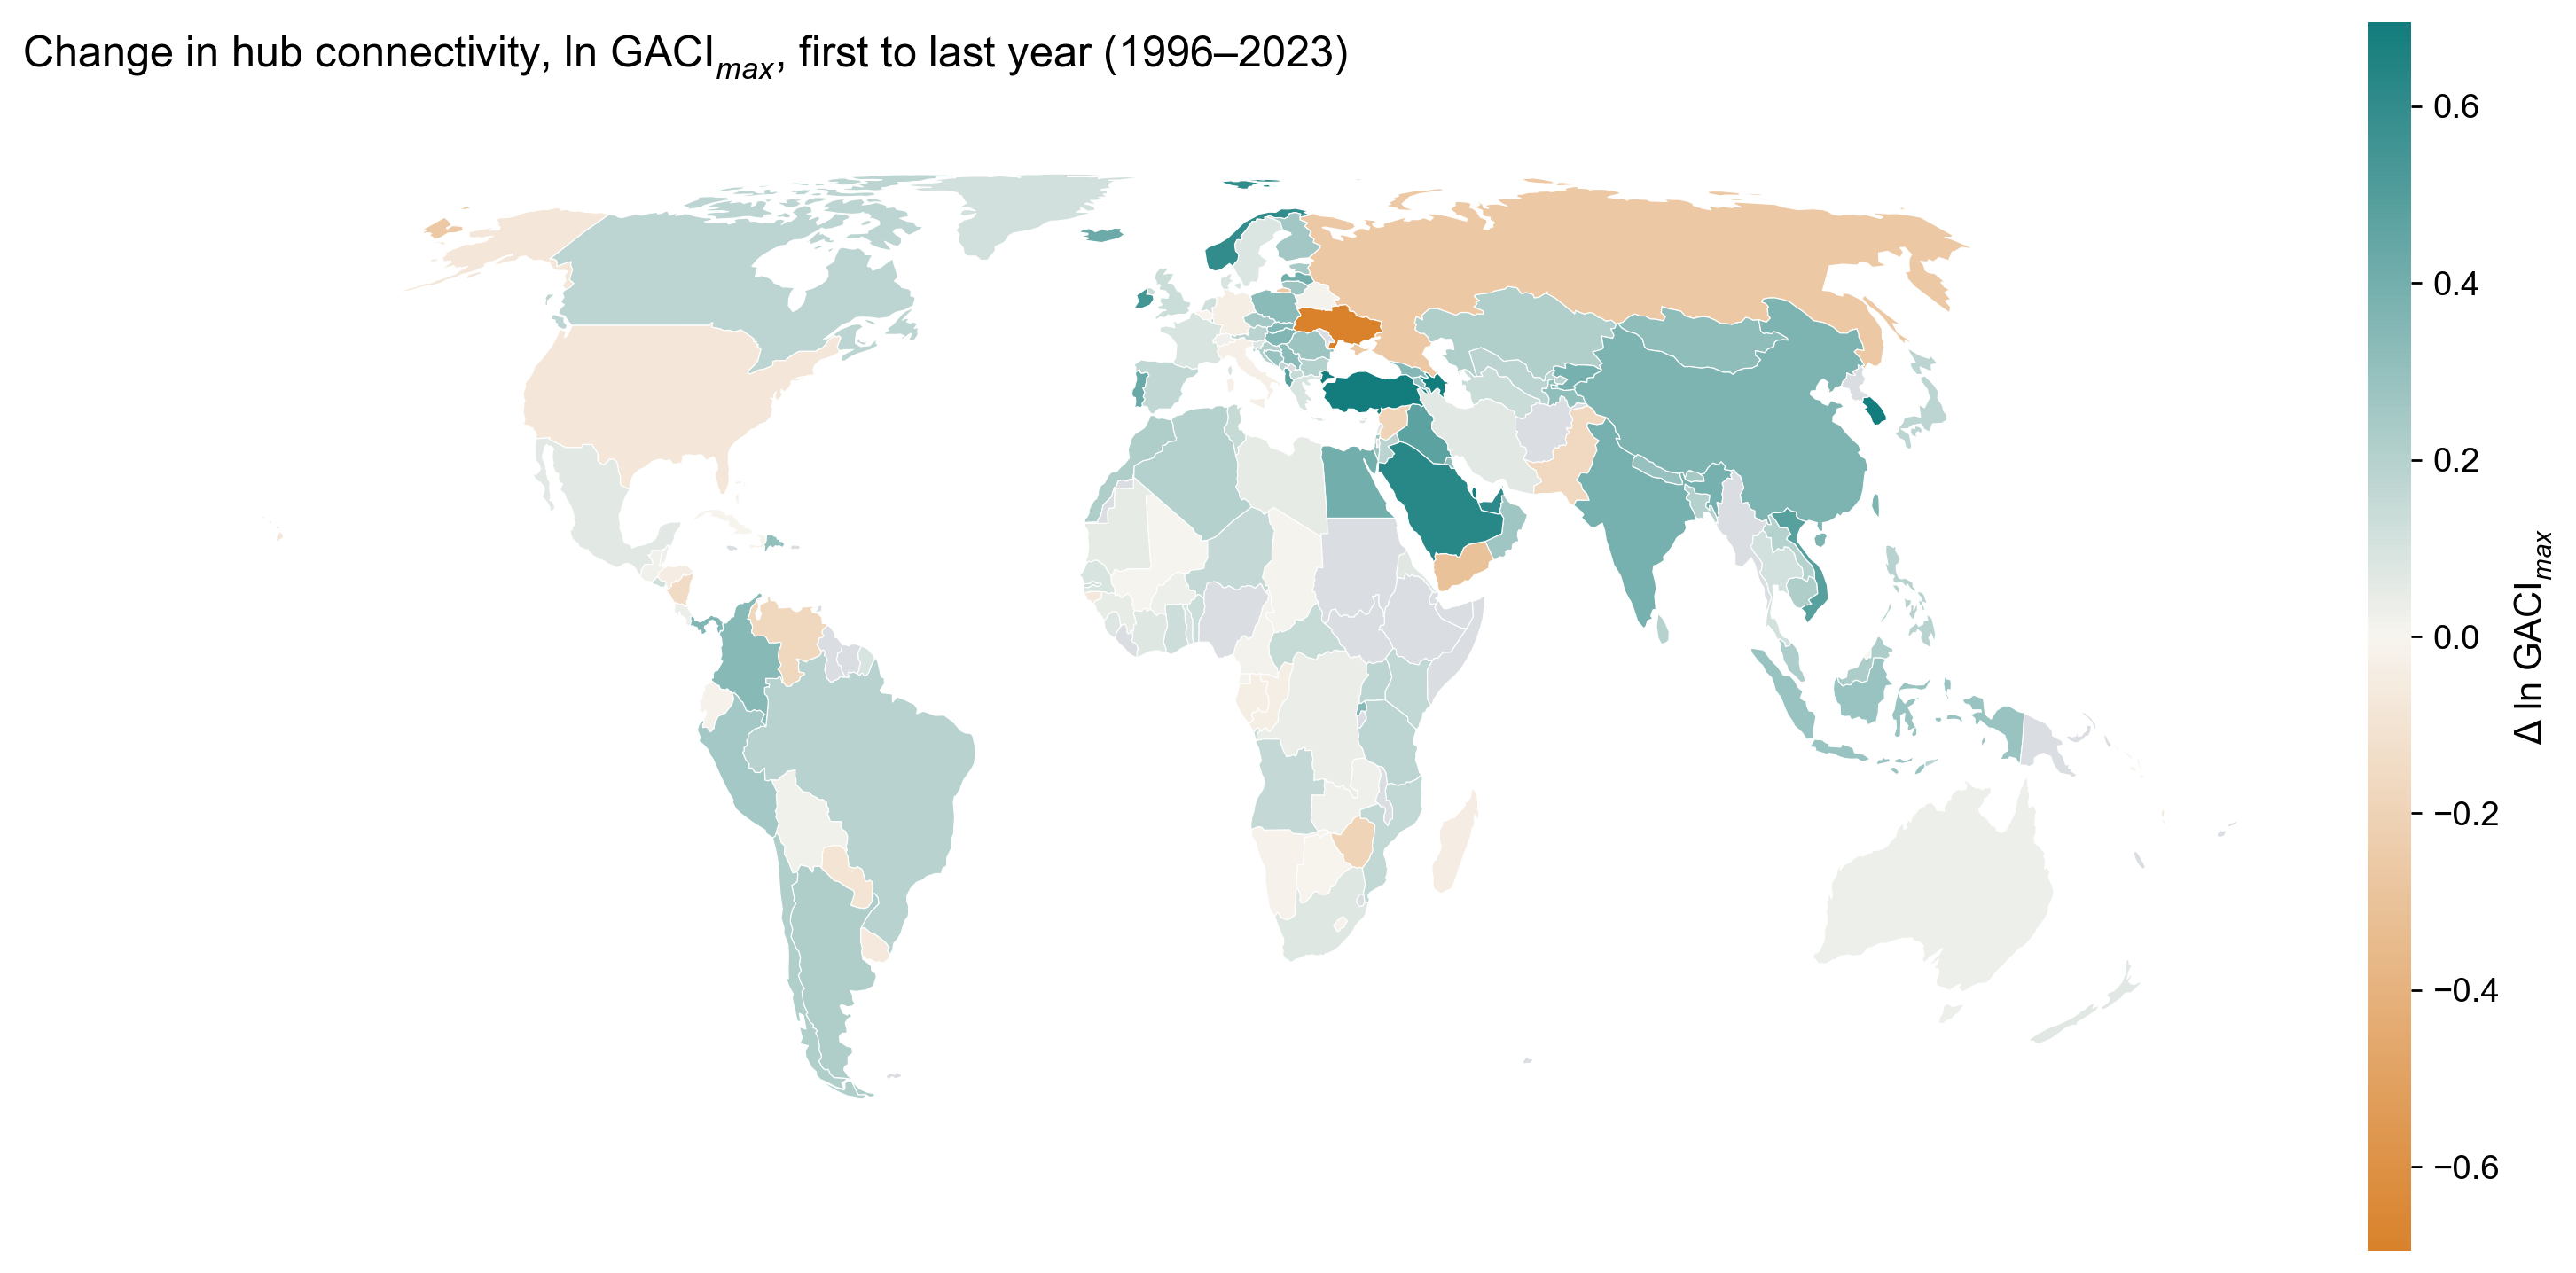
\includegraphics[width=\linewidth]{figures/FigB4_map_change.png}
\caption{Change in hub connectivity by country, $\ln\mathrm{GACI}_{max}$, between each country's first and last year in the panel (at least fifteen years apart; 147 countries). Teal denotes increases and amber decreases; grey denotes countries with fewer than fifteen years of data. Equal Earth projection.}
\label{fig:mapchange}
\end{figure}

This appendix also reports the supporting estimates referenced in the text. Table~\ref{tab:a_stage} reports the full set of incidence elasticities by baseline connectivity tercile, era and baseline GDP tercile. Table~\ref{tab:a_stacked} reports the stacked-system tests of equal group elasticities. Table~\ref{tab:a_lags} reports the headline estimate with connectivity lagged one to ten years. Table~\ref{tab:a_aggregate} reports the regional and world aggregates underlying Figure~\ref{fig:attribution}. Table~\ref{tab:a_regions} reports the market-Gini elasticity by macro region and by baseline inequality tercile; the regional first stages are weak outside Europe and Africa and the regional estimates should be read with that in mind. Tables~\ref{tab:a_stagedefs} and \ref{tab:a_stagedefs2} report the development-stage split under nine alternative definitions of the baseline. Table~\ref{tab:a_spill} reports the spillover specifications. Table~\ref{tab:a_components} reports the components of hub connectivity one at a time and in horse races. Table~\ref{tab:a_mediators} reports the mediation decomposition for eighteen candidate mediators.

\begin{table}[H]
\centering
\caption{Incidence by development stage: connectivity terciles, eras and GDP terciles (2SLS elasticities to $\ln\mathrm{GACI}_{max}$).}
\label{tab:a_stage}
\begin{minipage}{\linewidth}
\centering
\resizebox{\linewidth}{!}{%
\begin{tabular}{lccccccccc}
\toprule
 & & \multicolumn{3}{c}{Baseline connectivity tercile} & \multicolumn{2}{c}{Era} & \multicolumn{3}{c}{Baseline GDP p.c. tercile} \\
\cmidrule(lr){3-5}\cmidrule(lr){6-7}\cmidrule(lr){8-10}
 & Full sample & Low & Middle & High & 1996--2007 & 2010--23 ex. 2020--21 & Low & Middle & High \\
\midrule
ln market Gini & 0.495\sym{**} & 0.122 & 0.554\sym{**} & 1.410 & 0.214\sym{**} & 0.282\sym{*} & 0.337 & 0.591\sym{*} & 0.443\sym{*} \\
 & (0.194) & (0.096) & (0.219) & (2.308) & (0.095) & (0.167) & (0.619) & (0.343) & (0.255) \\
Mean income & 1.219\sym{**} & 1.520\sym{***} & 0.739 & 1.356 & 1.687\sym{***} & 1.114\sym{*} & 5.697 & 1.037 & 0.028 \\
 & (0.491) & (0.307) & (0.580) & (1.813) & (0.415) & (0.634) & (7.241) & (0.668) & (0.462) \\
Income, bottom 50\% & 0.445 & 1.727\sym{***} & -0.273 & -1.104 & 0.843\sym{*} & 0.838 & 4.139 & 0.417 & -0.915 \\
 & (0.593) & (0.396) & (0.660) & (4.037) & (0.471) & (0.694) & (5.513) & (1.006) & (0.807) \\
Income, top 10\% & 1.443\sym{***} & 1.328\sym{***} & 1.165\sym{**} & 1.909 & 1.845\sym{***} & 1.286\sym{*} & 5.962 & 1.062 & 0.438 \\
 & (0.513) & (0.395) & (0.594) & (2.440) & (0.408) & (0.688) & (7.389) & (0.760) & (0.443) \\
Share, bottom 50\% & -0.774\sym{*} & 0.206 & -1.011\sym{***} & -2.460 & -0.843\sym{**} & -0.277 & -1.558 & -0.620 & -0.943\sym{*} \\
 & (0.417) & (0.332) & (0.365) & (4.309) & (0.333) & (0.329) & (2.156) & (0.796) & (0.560) \\
Share, top 10\% & 0.224 & -0.192 & 0.427\sym{**} & 0.553 & 0.158 & 0.171 & 0.265 & 0.024 & 0.410 \\
 & (0.192) & (0.212) & (0.178) & (1.281) & (0.157) & (0.211) & (0.707) & (0.355) & (0.286) \\
Top half minus bottom half & 1.259\sym{*} & -0.169 & 1.496\sym{**} & 4.235 & 1.883\sym{**} & -0.530 & 3.242 & 1.034 & 1.385 \\
 & (0.755) & (0.314) & (0.643) & (7.720) & (0.770) & (0.625) & (4.438) & (1.275) & (1.228) \\
KP $F$ & 10.6 & 19.7 & 8.1 & 0.4 & 16.4 & 12.1 & 0.4 & 3.4 & 10.5 \\
Observations & 3{,}735 & 1{,}048 & 1{,}310 & 1{,}377 & 1{,}610 & 1{,}591 & 1{,}251 & 1{,}216 & 1{,}268 \\
\bottomrule
\end{tabular}}
\par\vspace{3pt}\begin{flushleft}\footnotesize Terciles on each country's earliest observed value. The high connectivity tercile and the low GDP tercile have no first stage (KP $F<1$) and are shown for completeness. Country-year panel, 1996--2023. All regressions include country and year fixed effects and log population. 2SLS instruments ln GACI with the Feyrer interaction $Z_{ct}=a_t\times\ln \mathrm{MA}^{air}_{c,1996}$. Standard errors clustered by country in parentheses. \sym{*}~$p<0.10$, \sym{**}~$p<0.05$, \sym{***}~$p<0.01$.\end{flushleft}
\end{minipage}
\end{table}

\begin{table}[H]
\centering
\caption{Stacked-system tests of equal group elasticities.}
\label{tab:a_stacked}
\begin{threeparttable}
\small
\begin{tabular}{lcc}
\toprule
 & OLS & 2SLS, Feyrer \\
\midrule
Joint test: equal elasticity across the ten deciles ($p$) & 0.188 & 0.735 \\
p90--100 minus p0--10 & 0.328\sym{**} & 1.288 \\
 & (0.155) & (1.613) \\
Top half minus bottom half & 0.051 & 1.296\sym{*} \\
 & (0.073) & (0.764) \\
Top 1\% minus p90--100 & 0.115\sym{*} & -0.157 \\
 & (0.064) & (0.274) \\
Linear trend: change in elasticity per decile & 0.013 & 0.256 \\
 & (0.016) & (0.164) \\
Linear trend: elasticity at the median decile & 0.620\sym{***} & 0.535 \\
 & (0.133) & (0.622) \\
\bottomrule
\end{tabular}
\begin{tablenotes}\small
\item All twelve WID groups stacked in one system (country $\times$ group $\times$ year) with group $\times$ ln GACI, group $\times$ log population, country $\times$ group and year $\times$ group fixed effects; each group's ln GACI is instrumented by group $\times$ $Z$. The linear-trend rows replace the group interactions by ln GACI and ln GACI $\times$ (decile rank $-5.5$) over the ten deciles. Per-equation KP $F$ = 10.5. Standard errors clustered by country.
\end{tablenotes}
\end{threeparttable}
\end{table}

\begin{table}[H]
\centering
\caption{Lagged connectivity (2SLS, Feyrer instrument).}
\label{tab:a_lags}
\begin{threeparttable}
\small
\begin{tabular}{lcccc}
\toprule
Lag of $\ln\mathrm{GACI}_{max}$ (years) & ln market Gini & ln disposable Gini & KP $F$ & N \\
\midrule
0 & 0.495\sym{**} & 0.651\sym{***} & 10.6 & 3{,}735 \\
 & (0.194) & (0.241) \\
1 & 0.471\sym{**} & 0.623\sym{***} & 10.7 & 3{,}568 \\
 & (0.184) & (0.228) \\
2 & 0.455\sym{**} & 0.617\sym{***} & 10.0 & 3{,}401 \\
 & (0.182) & (0.228) \\
3 & 0.464\sym{**} & 0.645\sym{**} & 9.1 & 3{,}236 \\
 & (0.200) & (0.250) \\
4 & 0.498\sym{**} & 0.689\sym{**} & 8.8 & 3{,}073 \\
 & (0.221) & (0.276) \\
5 & 0.513\sym{**} & 0.712\sym{**} & 7.9 & 2{,}912 \\
 & (0.234) & (0.296) \\
6 & 0.522\sym{**} & 0.729\sym{**} & 7.1 & 2{,}757 \\
 & (0.247) & (0.317) \\
7 & 0.511\sym{**} & 0.721\sym{**} & 6.4 & 2{,}604 \\
 & (0.254) & (0.332) \\
8 & 0.523\sym{*} & 0.745\sym{**} & 5.3 & 2{,}449 \\
 & (0.278) & (0.370) \\
9 & 0.479\sym{*} & 0.691\sym{**} & 5.2 & 2{,}296 \\
 & (0.259) & (0.344) \\
10 & 0.402\sym{*} & 0.588\sym{**} & 6.4 & 2{,}144 \\
 & (0.216) & (0.276) \\
\bottomrule
\end{tabular}
\begin{tablenotes}\small
\item Each row instruments the $k$-year lag of ln GACI with the $k$-year lag of $Z$. Country-year panel, 1996--2023. All regressions include country and year fixed effects and log population. 2SLS instruments ln GACI with the Feyrer interaction $Z_{ct}=a_t\times\ln \mathrm{MA}^{air}_{c,1996}$. Standard errors clustered by country in parentheses. \sym{*}~$p<0.10$, \sym{**}~$p<0.05$, \sym{***}~$p<0.01$.
\end{tablenotes}
\end{threeparttable}
\end{table}

\begin{table}[H]
\centering
\caption{Implied incidence of observed hub-connectivity growth, 1996 to latest year.}
\label{tab:a_aggregate}
\begin{minipage}{\linewidth}
\centering
\resizebox{\linewidth}{!}{%
\begin{tabular}{lrrrrrrrrrr}
\toprule
 & & & \multicolumn{2}{c}{Bottom-50 income, \%} & \multicolumn{2}{c}{Top-10 income, \%} & \multicolumn{2}{c}{Bottom-50 share, pts} & \multicolumn{2}{c}{Market Gini, pts} \\
\cmidrule(lr){4-5}\cmidrule(lr){6-7}\cmidrule(lr){8-9}\cmidrule(lr){10-11}
Region & N & $\Delta\ln\mathrm{GACI}$ & Implied & Actual & Implied & Actual & Implied & Actual & Implied & Actual \\
\midrule
Africa & 37 & 0.07 & 3.3 & 43.3 & 10.6 & 24.4 & -0.65 & 1.50 & 1.68 & -1.39 \\
Asia-Pacific & 23 & 0.22 & 9.6 & 72.0 & 31.1 & 78.8 & -2.43 & -0.72 & 4.76 & -0.95 \\
Europe & 42 & 0.22 & 9.9 & 57.1 & 32.0 & 59.0 & -3.02 & -0.08 & 5.47 & 1.47 \\
Latin America & 19 & 0.09 & 4.1 & 35.3 & 13.3 & 12.4 & -0.46 & 1.56 & 2.74 & -5.98 \\
Middle East & 9 & 0.22 & 9.8 & -15.7 & 31.6 & -8.7 & -1.51 & -0.37 & 5.09 & -2.27 \\
North America & 3 & 0.07 & 3.1 & 19.6 & 10.2 & 44.7 & -0.97 & -2.07 & 1.87 & 1.57 \\
Oceania & 5 & -0.07 & -3.0 & 17.6 & -9.6 & 36.5 & 1.10 & -1.29 & -1.40 & -0.96 \\
All (unweighted) & 138 & 0.15 & 6.6 & 45.9 & 21.5 & 41.1 & -1.64 & 0.36 & 3.61 & -1.06 \\
World (population-weighted) & 138 & 0.21 & 9.4 & 59.7 & 30.5 & 86.1 & -2.44 & -2.08 & 4.95 & 0.40 \\
\bottomrule
\end{tabular}}
\par\vspace{3pt}\begin{flushleft}\footnotesize Implied $=$ each country's change in $\ln\mathrm{GACI}_{max}$ between its first and last year with complete data ($\geq 15$ years apart; 138 countries) multiplied by the 2SLS elasticity of Table~\ref{tab:incidence} (income, in percent) or converted to share points using the share elasticity and the initial share; the Gini uses the elasticity of Table~\ref{tab:main}. Actual $=$ observed change over the same window. Continent rows are unweighted country means.\end{flushleft}
\end{minipage}
\end{table}

\begin{table}[H]
\centering
\caption{Heterogeneity by macro region and by baseline inequality (2SLS on subsamples).}
\label{tab:a_regions}
\begin{threeparttable}
\footnotesize
\begin{tabular}{lcccccc}
\toprule
 & ln market Gini & ln disp. Gini & Top half minus bottom half & Bottom-50 share & KP $F$ & N \\
\midrule
\multicolumn{7}{l}{\emph{Panel A. Macro region}}\\
Europe & -0.094 & -0.328\sym{*} & -0.942\sym{*} & 0.662\sym{**} & 7.2 & 1{,}131 \\
 & (0.211) & (0.199) & (0.500) & (0.328) \\
Asia-Pacific & 0.479\sym{*} & 0.365 & 0.572 & -0.912\sym{**} & 4.5 & 625 \\
 & (0.257) & (0.277) & (0.377) & (0.461) \\
Africa & -0.211 & -0.146 & -0.981 & 1.407 & 7.4 & 945 \\
 & (0.204) & (0.193) & (1.153) & (1.429) \\
Latin America & -0.079 & -0.515 & -3.217 & -0.076 & 0.7 & 556 \\
 & (0.950) & (0.961) & (8.727) & (1.982) \\
Middle East & 0.739 & 0.402 & -4.619 & 1.707 & 0.1 & 237 \\
 & (2.213) & (1.432) & (13.061) & (5.388) \\
\multicolumn{7}{l}{\emph{Panel B. Baseline market-Gini tercile}}\\
Low & 0.001 & 0.143 & -0.240 & 0.424 & 1.4 & 1{,}235 \\
 & (0.286) & (0.206) & (0.499) & (0.628) \\
Middle & 0.361 & 0.482 & 1.112 & -1.136 & 7.4 & 1{,}256 \\
 & (0.318) & (0.347) & (1.594) & (0.747) \\
High & 1.003 & 1.241 & 2.245 & -0.748 & 2.6 & 1{,}244 \\
 & (0.747) & (0.871) & (2.024) & (0.935) \\
\bottomrule
\end{tabular}
\begin{tablenotes}\small
\item Split-sample 2SLS. Regional first stages are weak outside Europe and Africa. Country-year panel, 1996--2023. All regressions include country and year fixed effects and log population. 2SLS instruments ln GACI with the Feyrer interaction $Z_{ct}=a_t\times\ln \mathrm{MA}^{air}_{c,1996}$. Standard errors clustered by country in parentheses. \sym{*}~$p<0.10$, \sym{**}~$p<0.05$, \sym{***}~$p<0.01$.
\end{tablenotes}
\end{threeparttable}
\end{table}

\begin{table}[p]
\centering
\caption{Development-stage split under alternative definitions of baseline hub size, $\mathrm{GACI}_{max}$ (2SLS elasticities to $\ln\mathrm{GACI}_{max}$).}
\label{tab:a_stagedefs}
\begin{minipage}{\linewidth}
\centering
\resizebox{\linewidth}{!}{%
\begin{tabular}{lccccccc}
\toprule
 & ln market Gini & Mean income & Top half minus bottom half & Bottom-50 share & Top-10 share & KP $F$ & N \\
\midrule
\multicolumn{8}{l}{\emph{$\mathrm{GACI}_{max}$ in 1996, terciles (baseline)}}\\
\quad Low & 0.122 & 1.520\sym{***} & -0.169 & 0.206 & -0.192 & 19.7 & 1{,}048 \\
 & (0.096) & (0.307) & (0.314) & (0.332) & (0.212) \\
\quad Middle & 0.554\sym{**} & 0.739 & 1.496\sym{**} & -1.011\sym{***} & 0.427\sym{**} & 8.1 & 1{,}310 \\
 & (0.219) & (0.580) & (0.643) & (0.365) & (0.178) \\
\quad High & 1.410 & 1.356 & 4.235 & -2.460 & 0.553 & 0.4 & 1{,}377 \\
 & (2.308) & (1.813) & (7.720) & (4.309) & (1.281) \\
\multicolumn{8}{l}{\emph{$\mathrm{GACI}_{max}$ in 1996, quartiles}}\\
\quad Q1 & 0.074 & 1.545\sym{***} & -0.146 & 0.189 & -0.212 & 20.3 & 752 \\
 & (0.099) & (0.319) & (0.245) & (0.290) & (0.178) \\
\quad Q2 & 0.720\sym{***} & 1.015\sym{*} & 1.504\sym{*} & -1.146\sym{***} & 0.519\sym{***} & 7.5 & 954 \\
 & (0.275) & (0.609) & (0.824) & (0.309) & (0.141) \\
\quad Q3 & 2.190 & -1.407 & 4.730 & -5.372 & 2.908 & 0.1 & 949 \\
 & (8.473) & (10.335) & (19.673) & (21.400) & (11.019) \\
\quad Q4 & 1.566 & 2.041 & 4.771 & -2.350 & 0.456 & 0.4 & 1{,}080 \\
 & (2.641) & (2.452) & (8.413) & (4.311) & (1.280) \\
\multicolumn{8}{l}{\emph{$\mathrm{GACI}_{max}$ in 1996, median split}}\\
\quad Below & 0.356\sym{***} & 1.318\sym{***} & 0.583 & -0.387 & 0.109 & 22.2 & 1{,}706 \\
 & (0.122) & (0.333) & (0.438) & (0.269) & (0.168) \\
\quad Above & 1.585 & 1.818 & 4.887 & -2.907 & 0.848 & 0.5 & 2{,}029 \\
 & (2.277) & (2.666) & (7.755) & (4.523) & (1.450) \\
\multicolumn{8}{l}{\emph{$\mathrm{GACI}_{max}$, mean 1996--2000, terciles}}\\
\quad Low & 0.256\sym{**} & 1.441\sym{***} & 0.568 & -0.187 & -0.013 & 30.8 & 1{,}031 \\
 & (0.101) & (0.290) & (0.546) & (0.392) & (0.227) \\
\quad Middle & 0.857 & 0.230 & 2.079 & -1.602 & 0.708 & 2.6 & 1{,}063 \\
 & (0.528) & (1.045) & (1.475) & (0.992) & (0.435) \\
\quad High & 1.229 & 2.046 & 3.107 & -2.001 & 0.417 & 0.6 & 1{,}186 \\
 & (1.821) & (2.083) & (5.484) & (3.221) & (1.035) \\
\multicolumn{8}{l}{\emph{$\mathrm{GACI}_{max}$, full-period mean, terciles}}\\
\quad Low & 0.241\sym{**} & 1.795\sym{***} & 0.326 & 0.064 & -0.154 & 17.3 & 1{,}025 \\
 & (0.103) & (0.334) & (0.520) & (0.383) & (0.218) \\
\quad Middle & 0.871 & 0.840 & 1.335 & -1.680 & 0.726 & 2.4 & 1{,}251 \\
 & (0.700) & (1.533) & (2.023) & (1.244) & (0.583) \\
\quad High & 0.607\sym{*} & 0.674 & 1.980 & -1.091 & 0.363 & 5.2 & 1{,}459 \\
 & (0.365) & (0.605) & (1.494) & (0.800) & (0.347) \\
\bottomrule
\end{tabular}}
\par\vspace{3pt}\begin{flushleft}\footnotesize Groups are formed over countries on the stated baseline variable. The instrument has power only in groups with small-to-moderate baseline hubs; wherever it has power the distributional pattern is the same. Country-year panel, 1996--2023. All regressions include country and year fixed effects and log population. 2SLS instruments ln GACI with the Feyrer interaction $Z_{ct}=a_t\times\ln \mathrm{MA}^{air}_{c,1996}$. Standard errors clustered by country in parentheses. \sym{*}~$p<0.10$, \sym{**}~$p<0.05$, \sym{***}~$p<0.01$.\end{flushleft}
\end{minipage}
\end{table}

\begin{table}[p]
\centering
\caption{Development-stage split under alternative baseline connectivity measures (2SLS elasticities to $\ln\mathrm{GACI}_{max}$).}
\label{tab:a_stagedefs2}
\begin{minipage}{\linewidth}
\centering
\resizebox{\linewidth}{!}{%
\begin{tabular}{lccccccc}
\toprule
 & ln market Gini & Mean income & Top half minus bottom half & Bottom-50 share & Top-10 share & KP $F$ & N \\
\midrule
\multicolumn{8}{l}{\emph{$\mathrm{GACI}_{cwm}$ in 1996, terciles}}\\
\quad Low & 0.116 & 1.667\sym{***} & 0.176 & 0.028 & -0.142 & 20.3 & 1{,}067 \\
 & (0.091) & (0.339) & (0.348) & (0.311) & (0.195) \\
\quad Middle & 2.154 & 2.304 & 7.621 & -3.911 & 1.213 & 0.7 & 1{,}288 \\
 & (2.468) & (2.820) & (9.239) & (4.573) & (1.311) \\
\quad High & 0.340 & 0.859 & -0.613 & -0.191 & 0.012 & 1.5 & 1{,}380 \\
 & (0.450) & (1.103) & (1.902) & (1.075) & (0.490) \\
\multicolumn{8}{l}{\emph{$\mathrm{GACI}_{sum}$ in 1996, terciles}}\\
\quad Low & 0.378\sym{**} & 0.998\sym{**} & 0.592 & -0.911\sym{***} & 0.381\sym{***} & 13.0 & 1{,}134 \\
 & (0.170) & (0.483) & (0.619) & (0.289) & (0.144) \\
\quad Middle & 0.334\sym{*} & 0.313 & 1.034 & -0.316 & 0.059 & 8.8 & 1{,}191 \\
 & (0.201) & (0.764) & (0.759) & (0.458) & (0.275) \\
\quad High & 0.655 & 1.603 & 1.969 & -1.016 & 0.205 & 1.7 & 1{,}410 \\
 & (0.566) & (1.146) & (2.110) & (1.072) & (0.468) \\
\multicolumn{8}{l}{\emph{Top-airport share of national GACI, 1996, terciles}}\\
\quad Low & 0.483 & 2.871 & 1.667 & -0.706 & -0.088 & 1.8 & 1{,}383 \\
 & (0.486) & (1.903) & (2.099) & (1.010) & (0.507) \\
\quad Middle & 0.805 & -0.827 & 1.902 & -0.873 & 0.412 & 2.8 & 1{,}221 \\
 & (0.525) & (1.513) & (1.679) & (0.997) & (0.555) \\
\quad High & 0.359\sym{**} & 0.814\sym{*} & 0.685 & -0.952\sym{***} & 0.413\sym{***} & 17.0 & 1{,}131 \\
 & (0.152) & (0.457) & (0.568) & (0.270) & (0.140) \\
\multicolumn{8}{l}{\emph{$\mathrm{GACI}_{max}$ in 1996, terciles within continent}}\\
\quad Low & 0.356\sym{**} & 0.773\sym{**} & 1.312\sym{***} & -0.803\sym{***} & 0.357\sym{***} & 12.5 & 1{,}199 \\
 & (0.143) & (0.380) & (0.433) & (0.230) & (0.101) \\
\quad Middle & 0.763 & 2.140 & 0.699 & -1.019 & 0.387 & 2.0 & 1{,}225 \\
 & (0.604) & (1.677) & (1.572) & (1.177) & (0.607) \\
\quad High & 0.846 & 0.269 & 2.701 & -1.132 & 0.080 & 2.2 & 1{,}234 \\
 & (0.737) & (1.078) & (2.827) & (1.413) & (0.546) \\
\bottomrule
\end{tabular}}
\par\vspace{3pt}\begin{flushleft}\footnotesize Groups are formed over countries on the stated baseline variable. The instrument has power only in groups with small-to-moderate baseline hubs; wherever it has power the distributional pattern is the same. Country-year panel, 1996--2023. All regressions include country and year fixed effects and log population. 2SLS instruments ln GACI with the Feyrer interaction $Z_{ct}=a_t\times\ln \mathrm{MA}^{air}_{c,1996}$. Standard errors clustered by country in parentheses. \sym{*}~$p<0.10$, \sym{**}~$p<0.05$, \sym{***}~$p<0.01$.\end{flushleft}
\end{minipage}
\end{table}

\begin{table}[p]
\centering
\caption{Spillovers from neighbours' connectivity.}
\label{tab:a_spill}
\begin{minipage}{\linewidth}
\centering
\resizebox{\linewidth}{!}{%
\begin{tabular}{lccccc}
\toprule
 & ln market Gini & ln disp. Gini & Top half minus bottom half & KP $F$ & N \\
\midrule
\multicolumn{6}{l}{\emph{Panel A. Own connectivity controlled}}\\
Own ln GACI exogenous; neighbours (inverse distance) & 1.648\sym{***} & 2.061\sym{***} & 4.010\sym{**} & 125.3 & 3{,}735 \\
 & (0.408) & (0.431) & (1.887) \\
Own shifter in reduced form; neighbours (inverse distance) & 4.648\sym{***} & 4.623\sym{***} & 8.187 & 32.3 & 3{,}735 \\
 & (1.245) & (1.183) & (5.581) \\
Joint 2SLS, contiguity: own ln GACI & 0.567\sym{**} & 0.685\sym{**} & 1.313\sym{*} & 4.0 & 3{,}735 \\
 & (0.227) & (0.285) & (0.797) \\
\quad neighbours' ln GACI & -0.099 & -0.047 & -0.075 & 4.0 & 3{,}735 \\
 & (0.135) & (0.204) & (0.458) \\
Joint 2SLS, within 500 km: own ln GACI & 0.407\sym{**} & 0.523\sym{**} & 0.678 & 5.6 & 3{,}735 \\
 & (0.179) & (0.214) & (0.669) \\
\quad neighbours' ln GACI & 0.084 & 0.121 & 0.550\sym{*} & 5.6 & 3{,}735 \\
 & (0.107) & (0.130) & (0.322) \\
Joint 2SLS, five nearest: own ln GACI & 0.367\sym{*} & 0.288 & 0.852 & 1.9 & 3{,}735 \\
 & (0.222) & (0.305) & (0.618) \\
\quad neighbours' ln GACI & 0.142 & 0.403 & 0.456 & 1.9 & 3{,}735 \\
 & (0.362) & (0.446) & (1.238) \\
Neighbours only (hybrid), contiguity & -0.175 & -0.139 & -0.248 & 184.8 & 3{,}735 \\
 & (0.109) & (0.101) & (0.318) \\
Neighbours only (hybrid), within 500 km & -0.042 & -0.041 & 0.339 & 37.6 & 3{,}735 \\
 & (0.122) & (0.130) & (0.387) \\
\multicolumn{6}{l}{\emph{Panel B. Distance decay (own shifter in reduced form)}}\\
500--1{,}000 km & 0.167 & 0.179 & 0.430 & 49.0 & 3{,}735 \\
 & (0.202) & (0.192) & (0.617) \\
1{,}000--2{,}000 km & -0.609\sym{**} & -0.605\sym{*} & 0.329 & 21.3 & 3{,}735 \\
 & (0.248) & (0.343) & (0.962) \\
2{,}000--5{,}000 km & 1.426\sym{*} & 1.574\sym{**} & 4.400\sym{*} & 16.3 & 3{,}735 \\
 & (0.746) & (0.727) & (2.531) \\
Kernel $\exp(-d/500\,\mathrm{km})$ & 0.710\sym{**} & 0.732\sym{**} & 1.532\sym{*} & 8.4 & 3{,}735 \\
 & (0.319) & (0.356) & (0.821) \\
Kernel $\exp(-d/1{,}000\,\mathrm{km})$ & 1.370\sym{**} & 1.325\sym{**} & 2.749\sym{*} & 13.8 & 3{,}735 \\
 & (0.543) & (0.549) & (1.437) \\
Kernel $\exp(-d/2{,}000\,\mathrm{km})$ & 2.969\sym{***} & 2.868\sym{***} & 6.052\sym{*} & 16.7 & 3{,}735 \\
 & (1.047) & (1.060) & (3.331) \\
\bottomrule
\end{tabular}}
\par\vspace{3pt}\begin{flushleft}\footnotesize Neighbour exposure is the leave-out weighted mean of other countries' ln GACI (capacity-weighted mean) under the stated weights, instrumented by the identically weighted mean of their Feyrer shifters; presence flags for neighbours are included. Wide-radius exposures average over most of a country's continent and are therefore less informative about neighbour-specific spillovers than the contiguity and 500 km definitions.Country-year panel, 1996--2023. All regressions include country and year fixed effects and log population. 2SLS instruments ln GACI with the Feyrer interaction $Z_{ct}=a_t\times\ln \mathrm{MA}^{air}_{c,1996}$. Standard errors clustered by country in parentheses. \sym{*}~$p<0.10$, \sym{**}~$p<0.05$, \sym{***}~$p<0.01$.\end{flushleft}
\end{minipage}
\end{table}

\begin{table}[p]
\centering
\caption{Components of hub connectivity.}
\label{tab:a_components}
\begin{minipage}{\linewidth}
\centering
\resizebox{\linewidth}{!}{%
\begin{tabular}{lcccccrr}
\toprule
 & ln market Gini & ln disp. Gini & Bottom-50 share & Top half minus bottom half & First stage & KP $F$ & N \\
\midrule
\multicolumn{8}{l}{\emph{Panel A. One hub component at a time, instrumented}}\\
GACI (composite) & 0.495\sym{**} & 0.651\sym{***} & -0.774\sym{*} & 1.259\sym{*} & 0.146\sym{***} & 10.6 & 3{,}735 \\
 & (0.194) & (0.241) & (0.417) & (0.755) & (0.045) \\
Seat capacity & 0.086\sym{***} & 0.113\sym{***} & -0.134\sym{**} & 0.217\sym{*} & 0.841\sym{***} & 22.9 & 3{,}735 \\
 & (0.030) & (0.034) & (0.063) & (0.118) & (0.176) \\
Number of connections & 0.128\sym{***} & 0.168\sym{***} & -0.198\sym{**} & 0.323\sym{*} & 0.567\sym{***} & 20.3 & 3{,}735 \\
 & (0.043) & (0.050) & (0.096) & (0.179) & (0.126) \\
Eigenvector centrality & 0.046\sym{***} & 0.060\sym{***} & -0.071\sym{**} & 0.116\sym{*} & 1.582\sym{***} & 37.8 & 3{,}735 \\
 & (0.015) & (0.016) & (0.032) & (0.061) & (0.257) \\
Closeness & 1.450\sym{***} & 1.907\sym{***} & -2.276\sym{**} & 3.703\sym{*} & 0.050\sym{***} & 12.2 & 3{,}735 \\
 & (0.504) & (0.623) & (1.140) & (2.098) & (0.014) \\
Flow betweenness & 0.348 & 0.457 & -0.530 & 0.852 & 0.208 & 0.7 & 3{,}735 \\
 & (0.432) & (0.558) & (0.679) & (1.099) & (0.253) \\
Regional importance & 0.151\sym{**} & 0.197\sym{***} & -0.231\sym{*} & 0.378\sym{*} & 0.477\sym{***} & 14.8 & 3{,}731 \\
 & (0.061) & (0.071) & (0.124) & (0.226) & (0.124) \\
\multicolumn{8}{l}{\emph{Panel B. Horse races on ln market Gini (component instrumented, another as control)}}\\
Eigenvector (IV) with seat capacity & 0.133\sym{**} (0.053) & -0.165\sym{**} (0.072) & \multicolumn{3}{l}{instrumented / control} & 22.2 & 3{,}735 \\
Seat capacity (IV) with betweenness & 0.089\sym{***} (0.030) & -0.011\sym{*} (0.007) & \multicolumn{3}{l}{instrumented / control} & 26.9 & 3{,}735 \\
Seat capacity (IV) with closeness & 0.148\sym{**} (0.065) & -1.037\sym{*} (0.543) & \multicolumn{3}{l}{instrumented / control} & 14.5 & 3{,}735 \\
Seat capacity (IV) with degree & 0.232\sym{*} (0.119) & -0.216\sym{*} (0.122) & \multicolumn{3}{l}{instrumented / control} & 7.3 & 3{,}735 \\
Degree (IV) with seat capacity & 0.526\sym{*} (0.298) & -0.269\sym{*} (0.157) & \multicolumn{3}{l}{instrumented / control} & 3.2 & 3{,}735 \\
Betweenness (IV) with seat capacity & -0.141\sym{**} (0.067) & 0.121\sym{**} (0.054) & \multicolumn{3}{l}{instrumented / control} & 6.9 & 3{,}735 \\
\bottomrule
\end{tabular}}
\par\vspace{3pt}\begin{flushleft}\footnotesize Hub $=$ the airport with the highest GACI in the country-year; components from the airport-level GACI panel. A single instrument moves every component (first-stage column), so one-at-a-time estimates are not separately identified; Panel B reports the pairwise horse races. Country-year panel, 1996--2023. All regressions include country and year fixed effects and log population. 2SLS instruments ln GACI with the Feyrer interaction $Z_{ct}=a_t\times\ln \mathrm{MA}^{air}_{c,1996}$. Standard errors clustered by country in parentheses. \sym{*}~$p<0.10$, \sym{**}~$p<0.05$, \sym{***}~$p<0.01$.\end{flushleft}
\end{minipage}
\end{table}

\begin{table}[H]
\centering
\caption{Candidate mediators: does the hub move them, and do they transmit the effect? (ln market Gini)}
\label{tab:a_mediators}
\begin{minipage}{\linewidth}
\centering
\resizebox{\linewidth}{!}{%
\begin{tabular}{lccccc}
\toprule
Mediator & $a$: hub $\rightarrow$ mediator (2SLS) & $c'$: hub with mediator held fixed & $b$: mediator & KP $F$ & N \\
\midrule
ln international tourist arrivals & 3.90\sym{**} (1.70) & 0.586\sym{**} (0.237) & -0.0272\sym{**} (0.0108) & 8.4 & 3{,}067 \\
Employment in industry, \% & 18.71\sym{*} (9.65) & 0.617\sym{**} (0.240) & -0.0058\sym{***} (0.0018) & 8.4 & 3{,}651 \\
Employment in agriculture, \% & -21.94\sym{*} (11.94) & 0.579\sym{**} (0.232) & 0.0032\sym{**} (0.0014) & 8.3 & 3{,}651 \\
Employment in services, \% & 3.23 (9.85) & 0.510\sym{**} (0.201) & -0.0004 (0.0012) & 9.9 & 3{,}651 \\
Urban population, \% & 12.13 (15.19) & 0.504\sym{***} (0.196) & -0.0007 (0.0013) & 10.8 & 3{,}735 \\
Trade, \% of GDP & 109.32\sym{*} (62.98) & 0.486\sym{**} (0.192) & 0.0001 (0.0001) & 10.0 & 3{,}725 \\
FDI inflows, \% of GDP & 27.49 (39.12) & 0.470\sym{***} (0.177) & 0.0000 (0.0000) & 12.1 & 3{,}679 \\
Wage and salaried workers, \% & 10.82 (8.17) & 0.549\sym{**} (0.222) & -0.0038\sym{*} (0.0020) & 9.1 & 3{,}651 \\
Unemployment rate, \% & 6.40 (6.29) & 0.479\sym{***} (0.182) & 0.0046\sym{***} (0.0014) & 11.2 & 3{,}651 \\
ln GDP per capita & 1.29\sym{***} (0.43) & 0.753\sym{**} (0.325) & -0.199\sym{**} (0.087) & 6.5 & 3{,}735 \\
Differentiated-goods share of trade & 0.33\sym{*} (0.17) & 0.533\sym{***} (0.205) & -0.084\sym{*} (0.047) & 10.4 & 3{,}723 \\
ln differentiated-goods trade & 2.97\sym{***} (1.11) & 0.705\sym{**} (0.300) & -0.067\sym{**} (0.027) & 6.5 & 3{,}723 \\
ln high value-to-weight trade & 2.66\sym{**} (1.04) & 0.652\sym{**} (0.269) & -0.055\sym{**} (0.022) & 7.3 & 3{,}723 \\
ln number of export partners & 1.94\sym{**} (0.96) & 0.586\sym{**} (0.250) & -0.0416\sym{*} (0.0232) & 7.5 & 3{,}723 \\
ln largest-city share of urban population & -0.18 (0.31) & 0.512\sym{**} (0.215) & -0.0053 (0.0573) & 9.3 & 3{,}270 \\
Labour share of income (PWT) & -0.12 (0.13) & 0.426\sym{***} (0.159) & -0.0272 (0.0906) & 14.8 & 2{,}655 \\
ln private credit, \% of GDP & 0.12 (0.92) & 0.514\sym{***} (0.196) & -0.0105 (0.0107) & 11.5 & 3{,}081 \\
Natural resource rents, \% of GDP & -9.92\sym{*} (5.24) & 0.472\sym{**} (0.189) & 0.0001 (0.0006) & 10.4 & 3{,}548 \\
\bottomrule
\end{tabular}}
\par\vspace{3pt}\begin{flushleft}\footnotesize $a$ is the 2SLS effect of $\ln\mathrm{GACI}_{max}$ on the mediator; $c'$ and $b$ come from the outcome equation with the mediator as a control and the hub instrumented. Mediators from the World Development Indicators, BACI (Rauch classification and unit values), and the Penn World Table. Country-year panel, 1996--2023. All regressions include country and year fixed effects and log population. 2SLS instruments ln GACI with the Feyrer interaction $Z_{ct}=a_t\times\ln \mathrm{MA}^{air}_{c,1996}$. Standard errors clustered by country in parentheses. \sym{*}~$p<0.10$, \sym{**}~$p<0.05$, \sym{***}~$p<0.01$.\end{flushleft}
\end{minipage}
\end{table}


\section*{Data and code availability}
The country-year connectivity panel is that of the companion papers. The SWIID and WID data are publicly available from \url{https://fsolt.org/swiid/} and \url{https://wid.world}. Stata and Python code reproducing every table and figure will be deposited in a public repository on acceptance.

\bibliographystyle{elsarticle-harv}
\bibliography{refs_inequality_v3}

\end{document}
